\documentclass[11pt,a4paper]{report}

\usepackage[a4paper,
			left=1.5in,
			right=1.5in,
			height=9.0in,
			headheight=14pt]{geometry}
\usepackage{fancyhdr}
\pagestyle{fancy}

\fancyhead[RE,LO]{\thepage}
\fancyhead[LE,RO]{\leftmark}

\usepackage{url}
\usepackage[utf8x]{inputenc}
\usepackage{ucs}
\usepackage{amsmath}
\usepackage{amsfonts}
\usepackage{amssymb}
\usepackage{graphicx}
\usepackage{natbib}
\usepackage{multicol}
\usepackage{subcaption}
\usepackage{makecell}
\usepackage[hidelinks]{hyperref}
\usepackage{rotating}
\usepackage[toc,page]{appendix}
\usepackage{epstopdf}
\usepackage{caption}
\usepackage{subcaption}
\newcolumntype{"}{@{\hskip\tabcolsep\vrule width 1pt\hskip\tabcolsep}}
\usepackage{enumitem}
\usepackage{float}

% Code snippet setup ---- START
\usepackage{listings}
\renewcommand{\lstlistingname}{Snippet}
\usepackage{color}
\definecolor{dkgreen}{rgb}{0,0.6,0}
\definecolor{gray}{rgb}{0.5,0.5,0.5}
\definecolor{light-gray}{rgb}{0.7,0.7,0.7}
\definecolor{lighter-gray}{rgb}{0.85,0.85,0.85}
\definecolor{mauve}{rgb}{0.58,0,0.82}
\lstset{frame=tb,
  language=Matlab,
  aboveskip=3mm,
  belowskip=3mm,
  showstringspaces=false,
  columns=flexible,
  basicstyle={\small\ttfamily},
  captionpos=b,
  numbers=left,
  numbersep=5pt,
  stepnumber=5,
  firstnumber=1,
  numberstyle=\tiny\color{gray},
  keywordstyle=\color{blue},
  commentstyle=\color{dkgreen},
  stringstyle=\color{mauve},
  breaklines=true,
  breakatwhitespace=false,
  tabsize=3
}
% Code snippet setup ---- END


%\title{{\LARGE \textbf{Design \& Analysis of Experiments}} \\
%{\LARGE Exam Assignment}\\
%{{\Large By group 403}}}
\begin{document}
\begin{titlepage}
\center % Center everything on the page
\newcommand{\HRule}{\rule{\linewidth}{0.5mm}} % Defines a new command for the horizontal lines, change thickness here


%----------------------------------------------------------------------------------------
%	HEADING SECTIONS
%----------------------------------------------------------------------------------------

\textsc{\LARGE Aalborg University Copenhagen}\\[1.5cm] % Name of your university/college
\textsc{\Large Design \& Analysis of Experiments}\\[0.5cm] % Major heading such as course name
\textsc{\large Group 403}\\[0.5cm] % Minor heading such as course title

%----------------------------------------------------------------------------------------
%	TITLE SECTION
%----------------------------------------------------------------------------------------

\HRule \\[0.4cm]
{ \huge \bfseries Exam Assignment}\\[0.4cm] % Title of your document
\HRule \\[1.5cm]

\vspace*{2\baselineskip} % Whitespace between location/year and editors

Authors: \\[\baselineskip]
{\Large Casper Sørensen \\ Daniel Christensen \\ Dina Madsen Smed \\ Emil Rose Høeg \\ Rasmus bloustrød Lind  \\ Sam Alix Nilsson \\ Simone Patricia Vinkel\par} % Editor list

\begin{minipage}{0.4\textwidth}
\author{
	Christensen, Daniel\\
	\and
	Høeg, Emil Rose \\
	\and
	Lind, Rasmus Bloustrød\\
	\and
	Nilsson, Sam Alix \\
	\and
	Smed, Dina Madsen\\	
	\and
	Sørensen, Casper\\
	\and
	Vinkel, Simone Patricia \\
}
\end{minipage}

\vspace*{15\baselineskip}
{\large \today}\\[3cm]

\end{titlepage}


%----------------------------------------------------------------------------------------
%	BUILD SECTION
%----------------------------------------------------------------------------------------
\newgeometry{twoside,left=1.5in,right=1.0in,height=9.0in, headheight=14pt}
\tableofcontents

\chapter{Statistical Questions}
% \section{Variables and Measurement}
 Choosing the right statistical tools for a test setup requires that one considers statistical methods and variables before even initiating the design. Basically it can be said that there are four types of variables to consider: 
\begin{itemize}
  \item Dependent variables
  \item Independent variables
  \item Discrete variables
  \item Continuous variables
\end{itemize}
Furthermore one must consider the levels of variables to be measured and analyzed in tests. Therefore it is important to keep in mind from the beginning which variables makes sense to analyze, and how the results can become useful. Eventually one collects data to understand how systems work, how products can be improved or how objects or actions causes change (causality) in e.g. defined environments. The fundamental understanding of these analytical terms will be shortly described in the following chapter.\\\\
Dependent variables are the values that are not being manipulated. They can also be described as the “outcome variables” \citep[page 21]{Design}. The measured values are dependant of of the other values in the system.\\\\
Independent variables are the values which can be said to be the “input variables”, which are the values that are being manipulated in a test environment. These variables are defined by the experimenter.
Discrete variables can be described as Boolean logic. The typical example for discrete variables is the pregnancy example on whether a woman is pregnant or not pregnant, and nothing in between \citep[page 9]{Design}.\\\\
Continuous variables can be scalable values that describes to what degree an event occurs or how much or how little something can be observed. Ratings and estimations are often defined as ratios. 
One must consider the above mentioned variable types before proceeding to the next step, that be the choice of data variables to place measurements in and to perform statistical analysis on. But before even considering data variable types, one must also distinguish between the two main categories as described in the next chapter: 
\begin{itemize}
\item Parametric
\item Non-parametric
\end{itemize}
Parametric data is considered to be the more powerful than its non-parametric equivalent \citep[page 21]{Design}, as it can be described as being: normally-distributed, based on arithmetic measurements of the continuous interval/ratio variable. The measurements are compareable as they represent concrete values measured by instruments or ratings.
Parametric Data Variables:
There are two fundamental data variables belonging to the parametric data types, which are described in the following chapter:
\begin{itemize}
\item Interval
\item Ratio 
\end{itemize}
Interval data are considered to be a preferred datatype from the ordinal data, and are also being utilized in psychological fields of study and research \citep[page 8]{Design}. Interval data are defined as being collected in an interval scale e.g used to describe feelings, moods and attitudes towards clearly specified questions, that be attempts to rate anxiety to scary animals. Interval data are often specified into a 10-point scale with equal values dividing the steps.\\\\
Ratio data are said to have the properties of interval data, but contains improved scalability and reveals differences into details. E.g. when measuring temperatures or to compare errors made by test subjects. Ratio data are particularly ideal for studies and research that require nuanced figures.\\\\
Non-parametric data are known to be free of assumptions as they do not meet the criterias contained in parametric data. That being said, non-parametric data contains elements of data with the characteristics of parametric data but are collected more randomly and commonly visualized into histograms. Typically collected data are analyzed and ranked, which can result in loss of detailed informations. 
\subsubsection{Non-parametric Data Variables:}
\begin{itemize}
\item Nominal
\item Ordinal
\end{itemize}
Nominal data are solely representing names for segments, players or numbers. They are not representing actual values but can be described as numerical semiotics e.g. in soccer the goal keeper is always playing with the number “1” and the attackers “10 \& 11”. Nominal data can not be considered as arithmetic but instead this type of data can be utilized to compare simular data segments for tests performed on e.g. pears or apples.\\\\
Ordinal Data are most oftenly used to describe when events occur e.g. who is first, second and third. This type of data does not indicate any other value and does not describe nuances nor important differences in specific values. Therefore this data type is not considered to be particularly useful as the most important information often lies in the details. 
\subsubsection{Statistical Tools}
With the above mentioned levels of data variables and types taken into consideration it is possible to make qualified choices of test scenarios and statistical methods. Whether analysis should be based on frequencies or scores, independent/dependant variables, experimental or correlational tests, parametric or non-parametric, groups and conditions, it is important to identify the purpose of the measurement and analysis. Considering these aspects one must choose between Chi-square, Pearsons, Spearmans, Anova, t-test etc. in order to collect the most useful results out of the performed tests with all the possible variables taken into consideration. For example, when having only one independent variable one would utilize the Chi-square, but when dealing with parametric or non-parametric data, one would choose between Pearson’s r and Spearman’s rho. It is of fundamental importance to consider these aspects as early as possible in order to understand and support the potential value of the tests \citep[page 274]{Design}.

\subsection{Question 1: Measurement}
\textit{Discuss levels on which variables could be measured. How the level of measurement influences the choice of statistical tools? (Hint: While answering this question, consult Chapter 8 of the book).}

\subsection{Question 2: Experimental Design}
\textit{In an experimental design, what do aims Reliability, Validity and Importance mean? Which actions should be taken to maximize measurements' reliability and validity?}

\subsection{Question 3: Analysis of Presented Data}
\textit{Analyze and present data gathered by a group of MED10 students for their semester project. Use available materials as a guideline and inspiration. Follow the document DAEV-ANOVA-exercises.pdf, and be sure to make all statistical tests mentioned there and to answer each of the points. Do all needed calculations and make all illustrative figures in Matlab.}

\subsection{Repetition: t-test}
% DESCRIPTION FOR POINT 1.1 -----------------------------------
\noindent\colorbox{light-gray}{\begin{minipage}{0.98\textwidth}
\textbf{1.1.} In a test of how gaming performance was affected by different kinds of feedback, 10 participants were measured. All participants played the game twice, once with auditory, and once with visual feedback. The type of feedback given first was counter-balanced across the group. The table below displays the measured time (in seconds) it took for the gamers to complete the final level of the game for the two conditions.
\end{minipage}}

% QUESTION 1.1 (1) --------------------------------------------
\noindent\colorbox{lighter-gray}{\begin{minipage}{0.98\textwidth}
\begin{enumerate}[label=\textbf{(\arabic*)}]\setcounter{enumi}{0}
	\item Should a one or two-tailed test be used if we want to know if there is a significant difference in gaming time between the two types of feedback? How many degrees of freedom?
\end{enumerate}\end{minipage}}

% ANSWER ------------------------------------------------------
\hspace{0pt} \\
In this test we are looking for a difference in the gaming time between the two types of feedback (auditory and visual). This means we do not have a specific hypothesis, e.g. that visual feedback would give a shorter gaming time. The tests should instead tell us if one or the other type of feedback is best. The null-hypothesis then states that there is no difference between auditory and visual feedback. We have now conducted that the test we are looking at is non-specific, thus we need to use a two-tailed test, where each tail would tell us if one or the other type of feedback would give us a shorter gaming time \citep[pp. 155-156]{Design}.

For each of the two samples of the feedback types 10 persons were tested giving a total of 20. The degrees of freedom for the overall test is thus the sum of the sample sizes minus one for each sample. The degrees of freedom for the samples are then 18 or 9 for each sample.

% QUESTION 1.1 (2) --------------------------------------------
\hspace{0pt} \\
\noindent\colorbox{lighter-gray}{\begin{minipage}{0.98\textwidth}
\begin{enumerate}[label=\textbf{(\arabic*)}]\setcounter{enumi}{1}
	\item Use the correct t-test and answer the question whether there is a significant difference (=.05).
\end{enumerate}\end{minipage}}

% ANSWER ------------------------------------------------------
\hspace{0pt} \\
Before we can do a t-test to test for a significant difference, we have to make sure that the samples come from normal distributions with a homogeneity of variance. First we test for homogeneity of variance between the two samples (auditory and visual feedback) using Bartlett's test. Here we assume that the population from which the two samples came are normal distributed. In the figure \ref{fig:2-1-1_vartestn} we see the statistics with a p-value supporting the null-hypothesis that the two samples do in fact have a homogeneity of variance. In the corresponding box plot, we can see that both samples have the approximately same properties such as the median and the inter-quartile range. These properties also suggests that the variances might be similar.

\begin{figure}[t]
	\centering
	\begin{subfigure}[t]{0.48\textwidth}
		\includegraphics[width=\textwidth]{fig/{2.1.1_vartestn_stats}.png}
		\caption{Statistics}
		\label{subfig:2-1-1_stats}
	\end{subfigure}
	\begin{subfigure}[t]{0.48\textwidth}
		\includegraphics[width=\textwidth]{fig/{2.1.1_vartestn_boxplot}.png}
		\caption{Boxplot}
		\label{subfig:2-1-1_boxplot}
	\end{subfigure}
	
	\caption{\textit{{\footnotesize Results from a Bartlett's test for equal variances. In \ref{subfig:2-1-1_stats} the p-value indicates that difference in the variances from the two samples are non-significant at the 0.05 level. The plot in \ref{subfig:2-1-1_boxplot} shows that the samples look very much alike with almost equal medians and inter-quartile ranges.}}}
	\label{fig:2-1-1_vartestn}
\end{figure}

Next we want to ensure that both samples come from a normal distributed population. For this we use the Kolmogorov-Smirnov test, where we standardize our samples and test for the null-hypothesis that the two samples come from standard normal distributions. The test yields the values $p=0.9811$ and $p=0.9897$ supporting the null-hypothesis.

Using a paired t-test on the two matched samples gives a p-value of $p=0.0319$ indicating that there is in fact a significant difference between the two types of feedback given (auditory and visual). With an alpha of $\alpha=0.05$ we can clearly determine that auditory feedback does not give the same gaming time as with visual feedback.

With all that said we have to take into account that we only have sample sizes of $N=10$. This means that even though the t-test rejects the null-hypothesis that there is no difference between the two types of feedback, it can be difficult to determine if it actually is the type of feedback that makes the difference and not some other factors. Andy Field \citep{Design} suggests that because a sample of a size beneath $N=30$ is messy, it can be difficult to determine.

% DESCRIPTION FOR POINT 1.2 -----------------------------------
\hspace{0pt} \\
\noindent\colorbox{light-gray}{\begin{minipage}{0.98\textwidth}
\textbf{1.2.} Download the zip archive 10ml883-data.zip containing text files with ratings on engagement from different experimental conditions as collected by group 10ml883. Start by importing the Engagement ratings for mouse and keyboard interfaces, as reported after 5 and 30 minutes of playing. Perform a t-test to compare if there is a difference in the rating of the intellectual engagement after 5 and 30 minutes of play.
\end{minipage}}

% QUESTION 1.2 (1) --------------------------------------------
\noindent\colorbox{lighter-gray}{\begin{minipage}{0.98\textwidth}
\begin{enumerate}[label=\textbf{(\arabic*)}]\setcounter{enumi}{0}
	\item What type of t-test should you use? Independent samples or paired?
\end{enumerate}\end{minipage}}

% ANSWER ------------------------------------------------------
\hspace{0pt} \\
If we assume that both samples are taken from observing the same 19 participants twice, the two samples are then dependent of each other. This means that we cannot use an independent t-test but instead we use a dependent paired t-test.

% QUESTION 1.2 (2) --------------------------------------------
\hspace{0pt} \\
\noindent\colorbox{lighter-gray}{\begin{minipage}{0.98\textwidth}
\begin{enumerate}[label=\textbf{(\arabic*)}]\setcounter{enumi}{1}
	\item What probability is there of obtaining these particular mean values purely by chance?
\end{enumerate}\end{minipage}}

% ANSWER ------------------------------------------------------
\hspace{0pt} \\
By following the same steps as above, we first need to validate that the samples have a homogeneity of variance and come from a normal distributed population. Testing for homogeneity of variance we get the results presented in figure \ref{fig:2-1-2_vartestn}. As we can see it seems that that the two samples do not have very similar variances giving us a problem when trying to use the t-test. If we then test for normal distribution of the two samples on 5 minutes and 30 minutes we get $p=0.0285$ and $p=0.0573$ correspondingly. These values indicates that the sample on 5 minutes does differ from a standard normal distribution while the 30 minutes sample does not. Again this would make a t-test less valid.

Doing the actual t-test will yield a p-value of $p=0.0031$ indicating a difference in intellectual engagement caused by the amount of time playing the game, i.e. 5 minutes or 30. However, since the validations of homogeneity of variance and of normal distribution, we might make a mistake stating that playing-time do make a difference.

\begin{figure}[h]
	\centering
	\begin{subfigure}[h]{0.48\textwidth}
		\includegraphics[width=\textwidth]{fig/{2.1.2_vartestn_stats}.png}
		\caption{Statistics}
		\label{subfig:2-1-2_stats}
	\end{subfigure}
	\begin{subfigure}[h]{0.48\textwidth}
		\includegraphics[width=\textwidth]{fig/{2.1.2_vartestn_boxplot}.png}
		\caption{Boxplot}
		\label{subfig:2-1-2_boxplot}
	\end{subfigure}
	
	\caption{\textit{{\footnotesize Results from a Bartlett's test for equal variances. The p-value seen in \ref{subfig:2-1-2_stats} tells there is a significant difference between the variances of the two samples. In boxes in \ref{subfig:2-1-2_boxplot} also shows a significant difference in the distribution of the observations in the two samples.}}}
	\label{fig:2-1-2_vartestn}
\end{figure}

% QUESTION 1.2 (3) --------------------------------------------
\hspace{0pt} \\
\noindent\colorbox{lighter-gray}{\begin{minipage}{0.98\textwidth}
\begin{enumerate}[label=\textbf{(\arabic*)}]\setcounter{enumi}{2}
	\item Is there a significant difference?
\end{enumerate}\end{minipage}}

% ANSWER ------------------------------------------------------
\hspace{0pt} \\
As explained above in 1.2 (2), yes there seems to be a significant difference.

% DESCRIPTION FOR POINT 1.3 -----------------------------------
\hspace{0pt} \\
\noindent\colorbox{light-gray}{\begin{minipage}{0.98\textwidth}
\textbf{1.3.} Now import the ratings for Wiimote after 30 minutes of playing. Proceed to explore the differences in Physical engagement between players using the mouse and keyboard interfaces, as compared to those using the Wii-mote. Test for differences in the ratings of Physical engagement between the two groups after 30 minutes of play.
\end{minipage}}

% QUESTION 1.3 (1) --------------------------------------------
\noindent\colorbox{lighter-gray}{\begin{minipage}{0.98\textwidth}
\begin{enumerate}[label=\textbf{(\arabic*)}]\setcounter{enumi}{0}
	\item What type of t-test should you use? Independent samples or paired?
\end{enumerate}\end{minipage}}

% ANSWER ------------------------------------------------------
\hspace{0pt} \\
Again we assume that the two samples uses the same 19 participants, thus the samples are dependent of each other. Therefore we must use a dependent/paired t-test.

% QUESTION 1.3 (2) --------------------------------------------
\hspace{0pt} \\
\noindent\colorbox{lighter-gray}{\begin{minipage}{0.98\textwidth}
\begin{enumerate}[label=\textbf{(\arabic*)}]\setcounter{enumi}{1}
	\item What probability is there of obtaining these particular mean values purely by chance?
\end{enumerate}\end{minipage}}

% ANSWER ------------------------------------------------------
\hspace{0pt} \\
Following the exact same steps we find that there is not any significant difference in the variances of the two samples given the data presented in figure \ref{fig:2-1-3_vartestn}. This is derived from the p-value of $p=0.788$ that clearly lies above the $0.05$ significance level. The test for normal distribution shows us that with the p-values of $p=0.1131$ and $p=0.1512$ the corresponding samples of the mouse \& keyboard and the Wii are deemed to belong to a normal distributed population.
Now we can perform the t-test between the two samples, which will give us a result of $p=0.00044$ clearly indicating a significant difference in physical engagement caused by changing the type of controller, i.e. mouse \& keyaboard or Wii.

\begin{figure}[h]
	\centering
	\begin{subfigure}[h]{0.48\textwidth}
		\includegraphics[width=\textwidth]{fig/{2.1.3_vartestn_stats}.png}
		\caption{Statistics}
		\label{subfig:2-1-3_stats}
	\end{subfigure}
	\begin{subfigure}[h]{0.48\textwidth}
		\includegraphics[width=\textwidth]{fig/{2.1.3_vartestn_boxplot}.png}
		\caption{Boxplot}
		\label{subfig:2-1-3_boxplot}
	\end{subfigure}
	
	\caption{\textit{{\footnotesize Results from a Bartlett's test for equal variances. Here the p-value in \ref{subfig:2-1-3_stats} indicates there is no significant difference in the variances, even though the boxes in \ref{subfig:2-1-3_boxplot} shows a very dissimilar distribution of the two samples.}}}
	\label{fig:2-1-3_vartestn}
\end{figure}

% QUESTION 1.3 (3) --------------------------------------------
\hspace{0pt} \\
\noindent\colorbox{lighter-gray}{\begin{minipage}{0.98\textwidth}
\begin{enumerate}[label=\textbf{(\arabic*)}]\setcounter{enumi}{2}
	\item Is there a significant difference?
\end{enumerate}\end{minipage}}

% ANSWER ------------------------------------------------------
\hspace{0pt} \\
As derived in 1.3 (2) there is a significant difference.
\subsection{Multiple Comparisons}
While t-test allows for the testing for cohesion between two mean values, it can often be insufficient when trying to calculate mean values of multiple test statistics. If more than two mean values are to be calculated, it must be done with pairwise testing. Every test increases the risk of committing type 1 errors i.e. accidentally rejecting a hypothesis that is actually true. Given a 5\% level of significance, the risk is thus 5\% per test. Therefore, if five mean values are to be tested (m1=m2=m3=m4=m5), the number of required tests would be 10, because all combinations must be executed. The combinatory conditions are calculated as follows:

\begin{equation}
\binom{n}{m} = {\frac{n!}{(m(m-n)!)}} 
\end{equation}\\
Meaning we will have the following amount of combinations:

\begin{equation}
\binom{5}{2} = {\frac{5!}{(2(5-2)!)}} = 10 
\end{equation}\\
This entails that every combination increases the probability of type 1 errors, and that the aggregated probability that type 1 error will be present in at least one of the tests is:

\begin{equation}
1-0,95^{10}= 1-0,599 = 40,1\%
\end{equation}\\
Hence, the probability  that at least one type 1 error will be present is approximately 40,1\%. The risk of committing a type 1 error will thus, increase explosively when the t-test is applied to mean-value comparisons of more than two populations.
\\

\subsection{Analysis of Variance (ANOVA)}
This increased risk can be very damaging for the credibility of any test; therefore it may be beneficial to eliminate as many confounding factors as possible. An \textit{analysis of variance}-test (ANOVA) may advantageously be used, as it is capable of comparing several mean values at once, and computing the variance.  To use ANOVA, one must apply the variance within each population as well as the variance between the populations. The formula for the 1-way ANOVA-test, also referred to as F-test, can thus be written:\\

\[F=\frac{between-group-variables}{within-group-variables}\]
\\
Thereby testing the mean value simultaneously rather than pairwise.
In the exercise (\textit{Design and Analysis of Experiments V: Exercies} by Sofia Dahl) three painkillers have to be compared to each other along with a placebo-version. Hence, there are four mean values that must be compared.  Instead of using the painkiller-data, we will analyse the data acquired by the 10th Semester group with a multiple comparison of means using the ANOVA-test, just like we have done in the previous assignments.
Since there are quite many dimensions of the aforementioned dataset, it is necessary to restrict ourselves to a few examples. Similar tests can be performed for all seven formats of engagement included in the data. But such a review would be comprehensive. If all combinations were to be tested we would have to test all of the three methods (MK, Wii and HMD) seven times, as well as seven times for each of the three time-entries (5,15 and 30) which would aggregate a total of 42 tests.
It is appropriate both logically and feasibly to start out with expanding the tests from exercice 1.2 and 1.3 to also include \textit{intellectual engagement for Mouse and Keyboard} after 15 minutes, and \textit{Physical engagement} for Head Mounted Display (HMD) after 30 minutes. Thus we have added an extra mean value that must be testet in the two tests, therefore we will use the one-way analysis of variance (ANOVA1 in MATLAB).\\

When using the ANOVA test a number of assumptions need to be fulfilled:
\begin{enumerate}
\item{The samples are normally distributed}
\item{The samples have the same variance (homogeneity of variance)}
\item{The samples are independent}
\end{enumerate}

Violations of assumption (1) can be acceptable, depending on how close the distribution is to the normal.
Violations of assumption( 2) will lead to inaccurate F-statistics. If the variances are significantly different, we can try to correct the problem by transforming the data or do a non-parametric test.
If assumption (3) is violated the F-statistics cannot be assumed to have an F-distribution. This means an increased probability of type II errors. 
Assumption (1) and (2) can be tested, whereas we have to look at the data in order to determine whether assumption (3) is a good assumption or not. In the case of the data from the 10th semester project, the samples cannot be assumed to be independent because it is the same 19 test subjects, that generates all the data. Hence, we need a new assumption:
(3a) Sphericity – the relationship between one pair of conditions is similar to the relationship of another pair of conditions \citep{Field_a}.
This assumption can be tested with the Mauchly’s test, which test the hypothesis, that the variance af the difference between conditions are equal \citep{Design}. Unfortunately we did not succeed in running this test in MATLAB, as the function is unknown. 
When using the repeated ANOVA, the test-statistics are generated using the variance within treatment and the variance between treatments.



\begin{figure}[h]
	\centering
	\begin{subfigure}[h]{0.48\textwidth}
		\includegraphics[width=\textwidth]{fig/{intellectualMK_testvalue}.png}
		\caption{Statistics}
		\label{IntellectMKtestVal}
	\end{subfigure}
	\begin{subfigure}[h]{0.48\textwidth}
		\includegraphics[width=\textwidth]{fig/{boxplotMK}.jpg}
		\caption{Boxplot}
		\label{intellectMK}
	\end{subfigure}
	
	\caption{{\footnotesize \textit{(a) Statistics shows the sum of squares (SS) which is the sum of the deviation in the power of 2, and degrees of freedom (DF) which is the number of “free” values that can be varied. The Mean Squares (MS) gives the average of the sum of squares SS/quantity, while the F-statistic (F) is the test statistic i.e. the measurements of the sample.The P-value (Prob$>$F) is The applied statistical probability that H0 is true in accordance with the f-statistic. (b) shows the notched boxplots generated by the test.}}}
	\label{ANOVA_1}
\end{figure}

In question 1.2 we tested the two samples (after 5 and 30 minutes) for normality, and we again perform the KS-test on the sample after 15 minutes. The KS-test shows, that we cannot reject the hypothesis, that the sample is normally distributed. As seen in the resulting figures of the ANOVA-test (fig. \ref{ANOVA_1}) we get a notched boxplot for the intellectual engagement after 5, 15 and 30 minutes. Although it is apparent that the medians are located similarly around 4 in the three groups, there are some considerable differences between them. After 5 minutes the grading ranges from 1 to 4, while after 15 and 30 minutes they range from 3 to 5. The notches in the figures specify the confidence interval (CI) around the mean, and it can tell us something about variance within each group. As previously specified one of the assumptions and requirements for the ANOVA-test is that there is similar variance (homogeneity of variance).  Although the variance after 5 and 15 minutes appears to be close to each other, the variance after 30 is less. The assumption of variance-cohesion can be tested with a Levene- variance test (vartestn in MATLAB), and the p-value from this test is 0,055 (5,5\%), hence we cannot reject that the three groups have the same variance.\\

The ANOVA table (fig. \ref{ANOVA_1}, (a) Statistics) generated by the one-way ANOVA-test generates an F-test statistic of 10,64 which gives a P-value of 0,0001 (0,001\%) which is way below our 5\% level of significance. Thus we can reject the null-hypothesis that there has been given similar grades for intellectual engagement after 5, 15 and 30 minutes.

\begin{figure}[h]
	\centering
	\begin{subfigure}[h]{0.48\textwidth}
		\includegraphics[width=\textwidth]{fig/{physical_testvalue}.png}
		\caption{Statistics}
		\label{PhysicalMKtestVal}
	\end{subfigure}
	\begin{subfigure}[h]{0.48\textwidth}
		\includegraphics[width=\textwidth]{fig/{BoxplotPhysical}.jpg}
		\caption{Boxplot}
		\label{PhysicaltMK}
	\end{subfigure}
	
	\caption{\textit{{\footnotesize (a) ANOVA Table and (b) Boxplot of the grades given for Physical Engagement after 30 minutes using the three types of controllers (mouse and keyboard, Wii and head mounted display).}}}
	\label{ANOVA_1.1}
\end{figure}

Figure \ref{ANOVA_1.1} shows the box plot for the grades given for Physical Engagement after 30 minutes using the three types of controllers. The median for HMD and MK are both 2, while Wii have a median of 3. The grades given range from 1 to 5 for both HMD and Wii, while MK only has one observation as high as 4 (in the boxplot it is regarded as an outlier). The notches indicate that the variance of the grades for HMD and Wii is larger than for MK. However, a variance test reveals a p-value of 0.905 indicating that we cannot reject the null-hypothesis of equal variance in the three samples. In question 1.3 we tested the two samples (physical engagement after 30 minutes for MK and Wii) and we test the last sample (HMD) as well and find that we cannot reject the hypothesis of normality. Hence, we continue with the ANOVA-test. This reveals an F-statistic of 7.31 which corresponds with a p-value of 0.0015 in the F-distribution with 2 DF. With a 5\% level of significance we reject the null-hypothesis that the three controllers are given the same score regarding physical engagement after 30 minutes.\\

A two-sided analysis of variance can test the effect of two factors simultaneously. The two-way ANOVA-test is performed for intellectual engagement after 5, 15 and 30 minuts for each of the three types of controllers. Hence, we test each factor (time and type of controller) alone (main effects) as well as the two factors combined (interaction). Thus we test if there is equal mean across time and type of controller as well as the interaction between them.

\begin{figure}[h]
	\begin{center}
		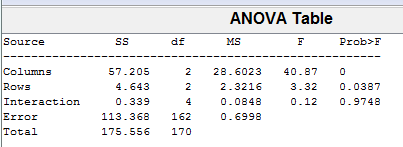
\includegraphics[height=3cm]{fig/anova2_testvalue.png}
		\caption{\textit{{\footnotesize Results for the two-sided ANOVA-test (anova2 in MATLAB) on intellectual engagement after 5, 15 and 30 minutes for each of the three types of controllers (mouse and keyboard, Wii and head mounted display).}}}
		\label{ANOVA_2}
	\end{center}
\end{figure}

The test (fig. \ref{ANOVA_2}) provides an F-statistic of 40.87 regarding the test across the columns (i.e. time). Hence, we can reject the hypothesis of equal mean grades for intellectual engagement after 5, 15 and 30 minutes. The test across the rows (types of controllers) provides an F-statistic of 3.32. In the F-distribution with 2 DF this corresponds with a p-value of 0.0387. With a 5\% level of significance we reject the hypothesis of equal mean for the three types of controllers. The last test has an F-statistic of 0.12 and a corresponding p-value of 0.9748. This provides evidence that there is no interaction between time and controller type in the grades given for intellectual engagement.

\chapter{Semester Project}
\textit{This question is about your group’s semester project.
First, state your final problem statement (this should be the same for all group members).
Make thorough analysis of your experimental design. Which are the elements that make your experiment a true scientific experiment? What was lacking, missing or which were less valid and reliable procedures? Make a proper justification of your experimental design choices!
Explain which data you collected and how, make needed statistical analysis and explain all conclusions.}
\section{Our Problem Statement}
Our final problem statement is: \textit{How can we automatically transcribe beatboxing}. To explain in other words: we record, analyse, and classify beatboxing according to part of the Standard Beatboxing Notation (SBN), more specifically the three beatboxing classes kick ('k'), snare ('s'), and highhat ('hh'). We implemented the system in Matlab.

Since we have quite a broad problem statement, there are many measures we could evaluate upon, as both audio features, segmentation, and classification are critical parts of our application. Even if only evaluating on the classifier, the number of combinations of features, and parameters of features (window size and window skip), is huge. We want keep a single independent variable. To limit ourselves, we chose not to test any combinations of features, but rather single features one at a time. We will then test that feature for $K \in [1;10]$. We state the null hypothesis that \emph{two knn-classifiers with a different k and otherwise identical, will not result in significantly different confusion tables}, and thus our alternative hypothesis is: \emph{two knn-classifiers with a different k and otherwise identical, will result in significantly different confusion tables.}


\subsection{True Scientific Experiment}
There are different elements determine our experiment are a true scientific experiment, in short elements are that our experiment are: measurable, testable, analyzable, falsifiable hypotheses and our experiment can be repeated.

In DAEBOOK XX REF the author talks about how Karl Popper see the difference between a scientific statement and a non-scientific statement. A non-scientific statement could sound like this: “Guys look better with makeup”. A statement like this is according to XX DEABOOK non-scientific, since it cannot be proven or disproved. Although most men do not wear makeup, and therefore one might claim the statement false. But since it cannot be tested and therefore only be judged by people subjectively. 
A scientific statement, on the other hand, can be tested and thereby confirmed or disconfirmed the statement as mentioned in XX DAEBOOK page 17. An example on a scientific statement could be like this: “Humans cannot without diver equipment breath under water“.
In our report the statement we used for our null hypothesis: "Two knn-classifiers with a different k and otherwise identical, will not result in significantly different confusion tables". 

This is a testable hypothesis and thereby also a scientific hypothesis. But as mentioned earlier, there are more to why it is a true scientific experiment. our hypothesis follows the falsification rule.

The falsification rule is when one try to disconfirm a hypothesis instead of trying to confirm the hypothesis. The method tells just as much as when one tries to confirm the hypothesis. Here is an example to help explaining  falsification. If our hypothesis sounded like this: all cats hate humans. If then one cat did not hate humans, then even if it is only one cat then the theory is disconfirmed. As field mentiones in DAEBOOK XX "one instance that disconfirms a hypothesis is more powerful than many instances that confirm the hypothesis."

Null hypothesis.
There are different kinds of hypothesis, one is called the experimental hypothesis, and another is called the null hypothesis. As explained in the DAEBOOK XX page 141 The experimental hypothesis predicts that your experiment will have an effect, where the null hypothesis prediction is wrong and there is no effect.
We use the null hypothesis to confirm or reject our experimental hypothesis. According to the DAEBOOK XX the experimental hypothesis or the null hypothesis can never be completely true, which is why when working with confirming or disconfirming experimental and null hypothesis, you work in percentages. For this percentage, Fisher suggest for a threshold for confidence we should use 95\% meaning that the experimental hypothesis is accepted when there is a 95\% certainty that the results are genuine.

Independend variables. 

When making an scientific experiment you are working with the manipulation of variables REF XX DAEBOOK page 21. The variables which is manipulated are what is called the independent variable. REF XX DAEBOOK the independent variable are different compared to the variables since its value is independent, the value is depended of the experimenter.
Then there is the dependent variables, their value depends on the rest of the variables in the experiment. The different variables is what John Stuart Mill proposed to be used to find casual factors. These could be found by comparing two condisions: one with supposed cause present, and one where it is not. XX DAEBOOK


validity vs reliybility

The theory behind falsifiability 


Make thorough analysis of your experimental design. Which are the elements that make your experiment a true scientific experiment?
\section{General Bias (what was lacking or what was less reliable/valid)}
%introduction
Here we will discus possible biases in our project, with focus on what biases that could effect the validity and reliability of our evaluation. We will first off discus how the data that was used in the project was collected, how the condition the collection took place and how the segmentation of the data for our program could have effected the results of the final evaluation of the data. Then we will discus what data was the output from the program will be shortly presented, then other methods of getting better data (we got mainly nominal data / frequency data) will be discussed.

%how was the data collected, problems with the data set e.g noise, how it was segmented and target group. also manual seg vs auto seg.
The data collected for this project was music files that contains Beatboxing from different participants. the participants were primary non beatboxers, they was found using convenience sampling method, which means that the participants was chosen based on proximity,  the fact that we did not consider their ability of beatboxing could contribute to making the validity less, because the way that the participants made beatboxing sounds made might not be correct to the sound that beatboxers with experience make. The collection took place on AAU campus Copenhagen at ac meyers vænge 15 in the main hall, the location of taken the main hall can contribute to more noise in the recordings which might will make the later classification different from recording at other places with less or more noise. next after the collection of the dataset we need to segment the audio to make a sound segments that contain the sound of beatboxing or noise, this was done in two way, one where it was eye balled to find the segments(using sonicvisualiser) and one where there was made use of a feature to find the sound segments(RMS). The segments that the two methods could be different in precision of how closely the segmentation can be (using sonic visualiser one can see on the waveform where the sound begins which can make a close segmentation, the RMS is taken in windows because of that one might get an overshoot of the sound), this can influence the classification of the segment sound section because one might contain more information than just the sound that we want to analyse. These different bias might contribute to validity of the later classification of the sound that then again effect the evaluation that we later did (chi squared).

%our test what we could have tested differently (we got frequency data any way that we could have gotten some kindof scale data instead perhaps with a test of executions speed, going out and make people try it to get there input into how correct they felt that their beatboxing was transcribed)

for the evaluation of our program matrices was made that shows the accuracy of the classifier with various settings and different features, secondly to make a statistical evaluation of the results we made chi squared test. The reason we used a chi squared test was that the data we collected from the classification program, the matrices, are categorized and they by that they are nominal data. To change that instead of focussing on how accurate the system is we could make a test of how fast the program is with the different features, this will give us different timings instead and this will give us ratio data which can give us more opportunities on what test we can use. 
%making the resoult less reliable, the target group only of non beatboxers, it might be that some of the people that helped us collect data had some experience and some non at all. bonfferroni


% Chapter 'Evaluation'

\section{Methods}
	\subsection{Hypothesis}
		In our project we tested several audio features and feature configurations.
		We tested window sizes of 20ms, 10ms, and 5ms; and window skips of 10ms, 5ms, 2ms respectively. This was the case for all features using windows: Mel Frequency Cepstral Coefficients (MFCC), Spectral Flux, Spectral Centroid, Spectral Skew, and Spectral Rolloff. Only the first 20 MFCC coefficients was used. The Root Mean Square (RMS) and Zero Crossing Rate (ZCR) was calculated over the entire sound.
		
		To determine if a difference in the independent variable $k$ had any significant effect on the resulting confusion tables (see Table \ref{table:eval:explanatory}), the chi squared test of association was used. This was done between two vectorized confusion tables calculated with all variables, except $k$, constant. We compared all resulting unique pairs of tables. Since we tested over 10 different K, but only on unique combinations of $K_1$ and $K_2$, the amount of tests done in total was $Tests = 10*9/2 = 45$. We have chosen that the null hypothesis can be disputed, if any calculated probability $p < \alpha$. Further, the Bonferroni correction\citep{bonferroni} will be applied to $\alpha=0.05$, such that $\alpha=\alpha/45 = 0.00\overline{1}$.
		
	\subsection{Measures}
		A confusion table was created for each test (each unique combination of variables). This was shown in percentages (or rather, on a scale from 0 and 1). Overall accuracy was calculated, along with precision, recall, and F-score for each sound class individually. For the sake of compactness, all the measures was included in an extended confusion table, as shown in the explanatory table \ref{table:eval:explanatory}. 
		The most important measure, for the sake of measuring our transcription system, would be the precision, that is, the amount of correctly transcribed sounds over the actual amount of that sound class.
		Recall should just be ignored, since we only test on the dataset, which means that we always test on all available samples of any given class, meaning that it would be the same as the total amount. This would be different, had the segmentation been part of the evaluation. When looking at results, we judged the performance primarily by accuracy and precision.

			\begin{table}
				\centering
				\begin{tabular}{|c | c | c | c | c |}
					\hline
				 & Real Class(1) & Real Class(2) & Real Class(3) & Precision\\ \hline
					Label(1)  & ... & ... & ... & ...\\ \hline
					Label(2)  & ... & ... & ... & ...\\ \hline
					Label(3) & ... & ... & ... & ...\\ \hline
					F-Score & ... & ... & ... & Accuracy \\ \cline{1-4}
				\end{tabular}
				\caption{$K=1$}
				\label{table:eval:explanatory}
			\end{table}
		
		
	\subsection{Data Collection}
	\label{sec:data-collecting}
	In order to build a system to transcribe beatboxing by amateurs, and in order to test said system, we had to create a dataset with many samples of beatboxing sounds. 
	Non-probability sampling was used to collect the data, in which 19 people participated, and it took place in the main building of Aalborg University Copenhagen. 
	
	The participants were placed in a chair surrounded by small partition walls (see cfigure \ref{data-collection-pic}) to limit noise from the surroundings. They were asked to produce 5-10 of each of the three types of sounds ('k', 's', 'hh'), and also to perform a self-improvised short mix of the sounds\footnote{This was done from a machine learning point-of-view, to better distinguish sounds with varying noise from other contemporary sounds.}
	
	To record the beatboxing sequences we used a e815-S dynamic cardioid microphone attached to an H4n portable recorder. The sampling rate was 96 kHz and 24 bit precision.
	
	The gathered data was collected on one track used as a database for our system. In order to utilize this database the sound file had to be manually annotated. This meant that for each sound its onset and duration was denoted and saved, and the type of sound labelled according to the three sound classes. This was done using Sonic Visualiser\footnote{\url{http://www.sonicvisualiser.org/}}, which generated a text file with the annotations.
	
	\begin{figure}[h]
		\begin{center}
			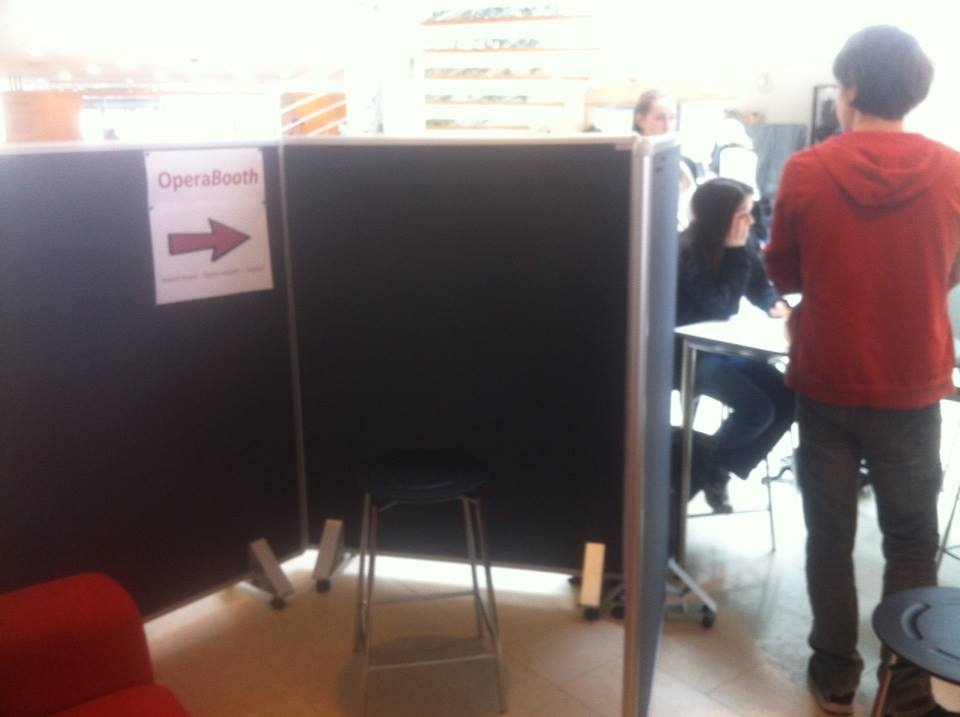
\includegraphics[height=5cm]{dataset_collection.JPG}
			\caption{Data collection booth.}
			\label{data-collection-pic}
		\end{center}
	\end{figure}
	
	
	\subsection{Training and Test Sets}
		The annotated beatboxing sound dataset used, consists of sound segments, segmented based on the manual annotations. The training and test sets of sound samples for the KNN classifier were randomly chosen from the same population (the dataset). It was distributed between the training and test set in a 70\%/30\% ratio, accordingly, for each class. This means there will not be a fixed number of sounds for each class (neither total nor divided), but rather a fixed distribution between the number of training and test sounds for each class. We can do this instead of e.g. k-fold cross validation, due to scale of our collected dataset. The ratio was suggested by our supervisor\footnote{Bob L. Sturm}. The composition of the entire dataset has been summarized in table \ref{table:eval:datasetComposition}. 
		Furthermore, all sounds with a duration less than the windowsize used for feature calculation, were removed before testing, since calculation was impossible on such short sounds. This was done before splitting the dataset, such as to make sure we did not distort the 70/30 distribution.

		\begin{table}
			\centering
			\begin{tabular}{|l|r|r|}
					\hline
					Value  &  Count  & Percent \\ \hline
			      noise    &  150    & 10.19\% \\ \hline
			          k    &  466    & 31.66\% \\ \hline
			  undefined    &  130    &  8.83\% \\ \hline
			          s    &  331    & 22.49\% \\ \hline
			         hh    &  395    & 26.83\% \\ \hline
			      TOTAL    &  1472	 & 100.00\% \\ \hline

			\end{tabular}
			\caption{Dataset composition}
			\label{table:eval:datasetComposition}
		\end{table}	
			
 
\section{Results}
	
	For all results found, some interpretation of the data and statistics will be presented, although it will be kept short due to the breadth of configurations tested. Only the relevant results will be shown and discussed, based on the accuracy, however the other measures will be considered as well. Results of the $X^2$ tests will be summarized and explained.asp\ref{app:RMS:9}). Some configurations had slightly higher precision in classes 's' and 'hh', although this seems minimal (see e.g. appendix  \ref{app:rms:k6} and \ref{app:rms:k8}). The worst observed was using $K=1$, with accuracy 53.9\% see appendix \ref{app:RMS:1:worst}. All results from for the RMS feature can be found in appendix \ref{app:res:rms}. The $X^2$ test revealed no significant differences between any two $K$ (see all p in \ref{xlrms11}).

		
	%
	%	ZCR
	%
	
	\subsection{Zero Crossing Rate}
%		\begin{figure}
%			\centering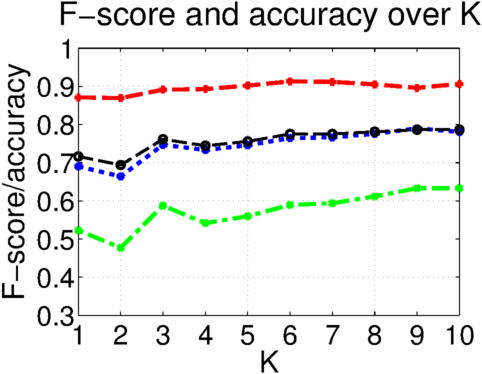
\includegraphics[width=0.3\textwidth]{tex/appendices/test/zcr11FP.png}
%			\centering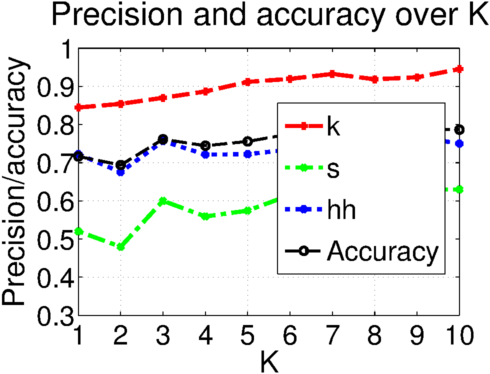
\includegraphics[width=0.3\textwidth]{tex/appendices/test/zcr11_P.png}
%			\centering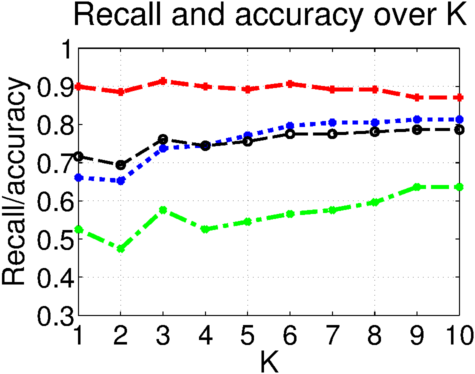
\includegraphics[width=0.3\textwidth]{tex/appendices/test/zcr11_R.png}
%			\label{fig:eval:zcr}
%			\caption{Plots over K for Zero Crossing Rate}
%		\end{figure}
%		
%		\begin{table}
%			\begin{subtable}[tbp]{0.45\textwidth}
%				\centering
%				\begin{tabular}{|c|c|c|c"c|}
%					\cline{2-5}
%					 \multicolumn{1}{c|}{} & \textbf{k}  & \textbf{s}  & \textbf{hh}  & Prec.\\ \hline
%					 \textbf{k} & \textcolor{red}{0.871} & 0.081 & 0.017 & 0.924\\ \hline
%					 \textbf{s} & 0.122 & \textcolor{red}{0.636} & 0.169 & 0.630\\ \hline
%					 \textbf{hh} & 0.122 & 0.283 & \textcolor{red}{0.814} & 0.768\\ \Xhline{2\arrayrulewidth}
%					 F & 0.896 & 0.633 & 0.790 & \textcolor{blue}{0.787}\\ \hline
%				\end{tabular}
%				\label{table:eval:zcrBest1}
%				\caption{$K=9$ (Best)}
%			\end{subtable}
%		
%			\begin{subtable}[tbp]{0.45\textwidth}
%				\centering
%				\begin{tabular}{|c|c|c|c"c|}
%					\cline{2-5}
%					 \multicolumn{1}{c|}{} & \textbf{k}  & \textbf{s}  & \textbf{hh}  & Prec.\\ \hline
%					 \textbf{k} & \textcolor{red}{0.871} & 0.051 & 0.017 & 0.945\\ \hline
%					 \textbf{s} & 0.122 & \textcolor{red}{0.636} & 0.169 & 0.630\\ \hline
%					 \textbf{hh} & 0.122 & 0.313 & \textcolor{red}{0.814} & 0.750\\ \Xhline{2\arrayrulewidth}
%					 F & 0.906 & 0.633 & 0.780 & \textcolor{blue}{0.787}\\ \hline
%				\end{tabular}
%				\label{table:eval:zcrBest2}
%				\caption{$K=10$ (Best)}
%			\end{subtable}
%			
%			\begin{subtable}[tbp]{0.45\textwidth}
%				\centering
%				\begin{tabular}{|c|c|c|c"c|}
%					\cline{2-5}
%					 \multicolumn{1}{c|}{} & \textbf{k}  & \textbf{s}  & \textbf{hh}  & Prec.\\ \hline
%					 \textbf{k} & \textcolor{red}{0.885} & 0.162 & 0.042 & 0.854\\ \hline
%					 \textbf{s} & 0.108 & \textcolor{red}{0.475} & 0.305 & 0.480\\ \hline
%					 \textbf{hh} & 0.108 & 0.364 & \textcolor{red}{0.653} & 0.675\\ \Xhline{2\arrayrulewidth}
%					 F & 0.869 & 0.477 & 0.664 & \textcolor{blue}{0.694}\\ \hline
%				\end{tabular}
%				\label{table:eval:zcrWorst}
%				\caption{$K=2$ (Worst)}
%			\end{subtable}
%			
%			\caption{Measures over K using ZCR}
%		\end{table}
		

		The best results using ZCR was a tie between $K=9$ (appendix \ref{app:zcr:best}) and $k=10$ (appendix \ref{app:zcr:best2}), both with accuracy 78.7\%. In the results from $K=9$, the precision of the hh is slightly better than in $K=10$ (75\% vs 67.5\%). In $K=10$, the precision of the kick is slightly better (94.6\% vs 92.4\%). The worst results was observed with $K=2$, having accuracy 69.4\%(appendix \ref{app-ZCR-Worst}). No tests were deemed significant by $X^2$ testing. See all $X^2$ results in appendix \ref{xlzcr11}.
		
	%	
	%	MFCC
	%	
		
	\subsection{Mel Frequency Cepstrum Coefficients}
%		\begin{figure}
%			\centering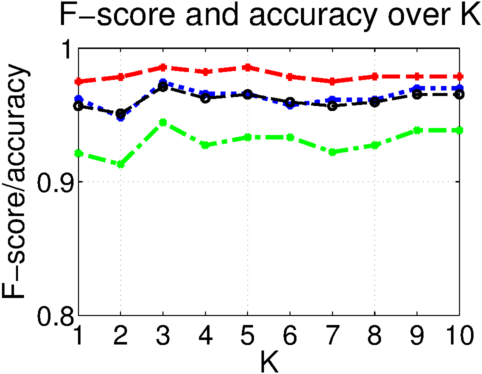
\includegraphics[width=0.3\textwidth]{tex/appendices/test/mfcc2010FP.png}
%			\centering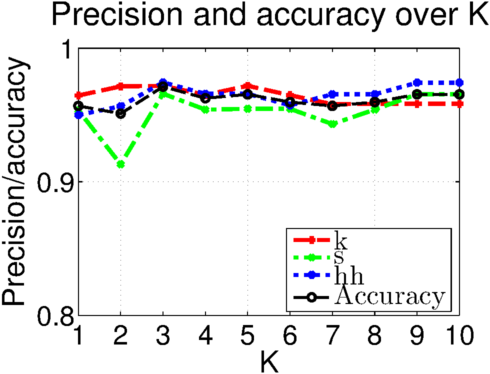
\includegraphics[width=0.3\textwidth]{tex/appendices/test/mfcc2010_P.png}
%			\centering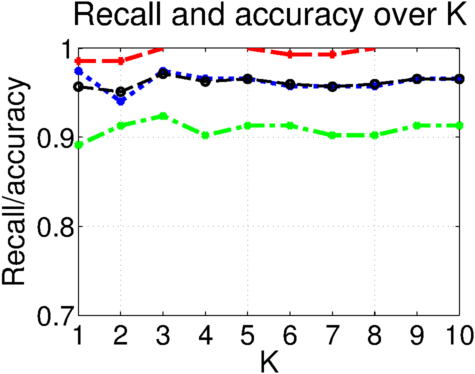
\includegraphics[width=0.3\textwidth]{tex/appendices/test/mfcc2010_R.png}
%			
%			\caption{Plots over K for MFCC with 20ms windows and 10ms window skips}
%		\end{figure}
%		\begin{figure}
%			\centering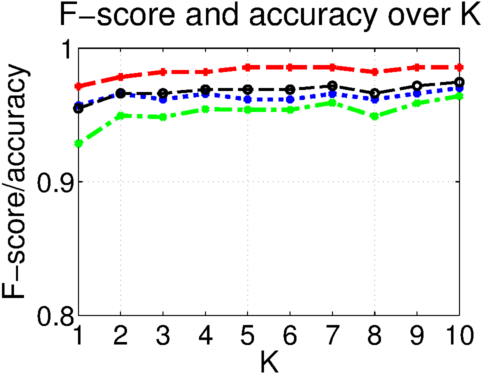
\includegraphics[width=0.3\textwidth]{tex/appendices/test/mfcc105FP.png}
%			\centering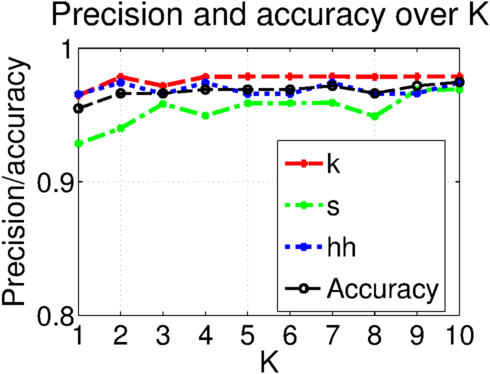
\includegraphics[width=0.3\textwidth]{tex/appendices/test/mfcc105_P.png}
%			\centering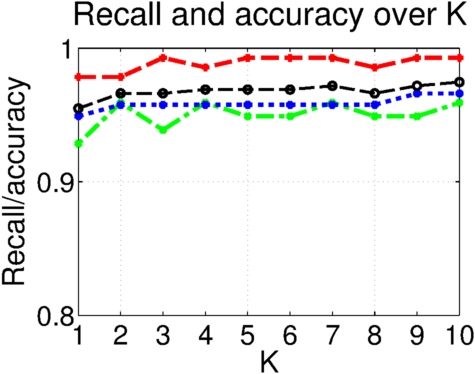
\includegraphics[width=0.3\textwidth]{tex/appendices/test/mfcc105_R.png}
%			
%			\caption{Plots over K for MFCC with 10ms windows and 5ms window skips}
%		\end{figure}
%		\begin{figure}
%			\centering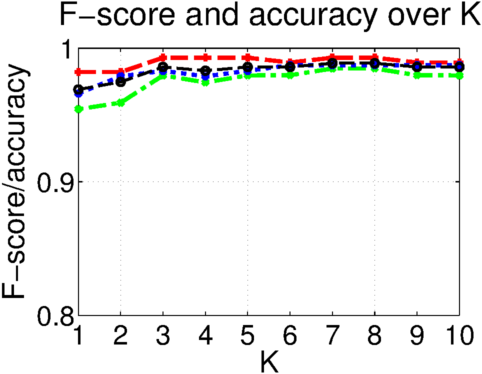
\includegraphics[width=0.3\textwidth]{tex/appendices/test/mfcc52FP.png}
%			\centering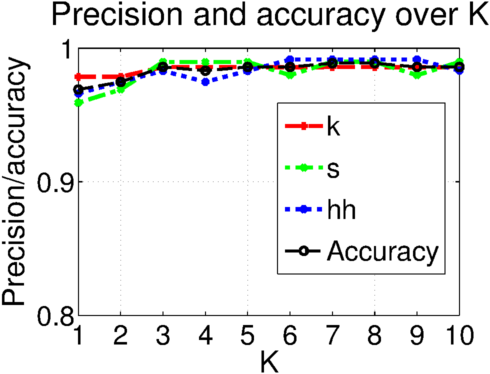
\includegraphics[width=0.3\textwidth]{tex/appendices/test/mfcc52_P.png}
%			\centering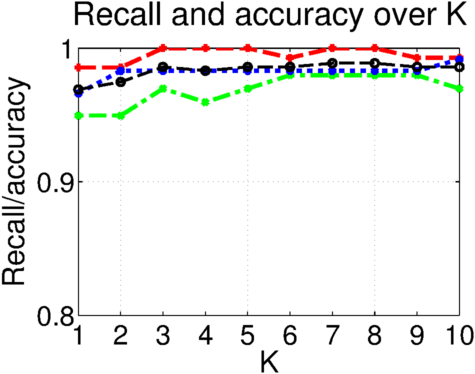
\includegraphics[width=0.3\textwidth]{tex/appendices/test/mfcc52_R.png}
%			
%			\caption{Plots over K for MFCC with 5ms windows and 2ms window skips}
%		\end{figure}\clearpage
%		
%		\begin{table}
%			\begin{subtable}[tbp]{0.45\textwidth}
%				\centering
%				\begin{tabular}{|c|c|c|c"c|}
%					\cline{2-5}
%					 \multicolumn{1}{c|}{} & \textbf{k}  & \textbf{s}  & \textbf{hh}  & Prec.\\ \hline
%					 \textbf{k} & \textcolor{red}{1.000} & 0.010 & 0.008 & 0.986\\ \hline
%					 \textbf{s} & 0.000 & \textcolor{red}{0.980} & 0.008 & 0.990\\ \hline
%					 \textbf{hh} & 0.000 & 0.010 & \textcolor{red}{0.983} & 0.991\\ \Xhline{2\arrayrulewidth}
%					 F & 0.993 & 0.985 & 0.987 & \textcolor{blue}{0.989}\\ \hline
%				\end{tabular}
%				\caption{$wSize=5ms, wSkip=2ms, K=7$}
%				\label{table:eval:mfccBest1}
%			\end{subtable}
%			\hfill
%			\begin{subtable}[tbp]{0.45\textwidth}
%				\centering
%				\begin{tabular}{|c|c|c|c"c|}
%					\cline{2-5}
%					 \multicolumn{1}{c|}{} & \textbf{k}  & \textbf{s}  & \textbf{hh}  & Prec.\\ \hline
%					 \textbf{k} & \textcolor{red}{1.000} & 0.010 & 0.008 & 0.986\\ \hline
%					 \textbf{s} & 0.000 & \textcolor{red}{0.980} & 0.008 & 0.990\\ \hline
%					 \textbf{hh} & 0.000 & 0.010 & \textcolor{red}{0.983} & 0.991\\ \Xhline{2\arrayrulewidth}
%					 F & 0.993 & 0.985 & 0.987 & \textcolor{blue}{0.989}\\ \hline
%				\end{tabular}
%				\caption{$wSize=5ms, wSkip=2ms, K=8$}
%				\label{table:eval:mfccBest2}
%			\end{subtable}
%			\hfill
%			\begin{subtable}[tbp]{0.45\textwidth}
%			\centering
%			\begin{tabular}{|c|c|c|c"c|}
%			\cline{2-5}
%			 \multicolumn{1}{c|}{} & \textbf{k}  & \textbf{s}  & \textbf{hh}  & Prec.\\ \hline
%			 \textbf{k} & \textcolor{red}{0.986} & 0.043 & 0.000 & 0.971\\ \hline
%			 \textbf{s} & 0.007 & \textcolor{red}{0.913} & 0.060 & 0.913\\ \hline
%			 \textbf{hh} & 0.007 & 0.043 & \textcolor{red}{0.940} & 0.957\\ \Xhline{2\arrayrulewidth}
%			 F & 0.978 & 0.913 & 0.948 & \textcolor{blue}{0.951}\\ \hline
%			\end{tabular}
%			\caption{$wSize=20ms, wSkip=10ms, K=2$}
%			\label{table:eval:mfccWorst}
%			\end{subtable}
%			
%			\caption{Measures over K using MFCC}
%		\end{table}
		

		Over all three configurations of the MFCC feature vector, the best performing were $K=7$ and $K=8$ with accuracies 98.9\%, when using a window size of 5ms and skip of 2ms (see appendix \ref{app:MFCC:7:best} and \ref{app:MFCC:8:best}). Some of the other results with the same parameters reach similar performance in regards to precision per class (see appendix \ref{tlmfcc52}). The worst performing, with 95.1\% accuracy, is using 20ms window size and 10ms skip with $K=2$ (see appendixs \ref{app:Mfcc:2:worst}). It still has better precision for kick than some others(e.g. $K=4$ or $K=6$), but some have similar hh precision (e.g. $K=1$ or $K=6$). No $X^2$ results were considered significant (although some came quite close; see appendix \ref{xlmfcc52}).
		
	%
	% SC
	%
	\subsection{Spectral Centroid}

		Using the Spectral Centroid feature, the best configuration found, with accuracy 82.8\% was 10ms windows and 5ms window skips, and $K=9$, as shown in appendix \ref{app:sc:9:best}. Some results show similar or better precision in some classes, e.g. $K=8$. The worst accuracy seen, was usisng 20ms window size, 10ms window skip, and $K=2$, with accuracy 73.8\%, as shown in table \ref{app:SC:2:worst}. $X^2$-test revealed no significant differences (see all in appendix \ref{app:res:sc}).
		
				
	% 
	% SS
	%
	\subsection{Spectral Skew}
			
%		\begin{figure}
%			\centering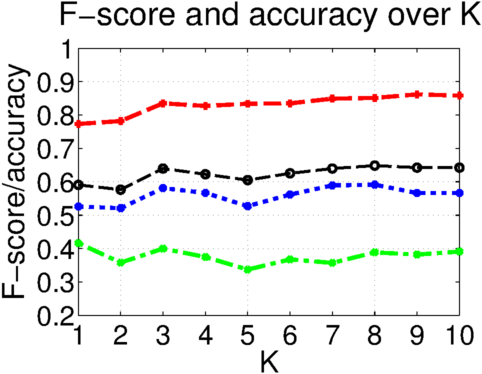
\includegraphics[width=0.3\textwidth]{tex/appendices/test/sskew2010FP.png}
%			\centering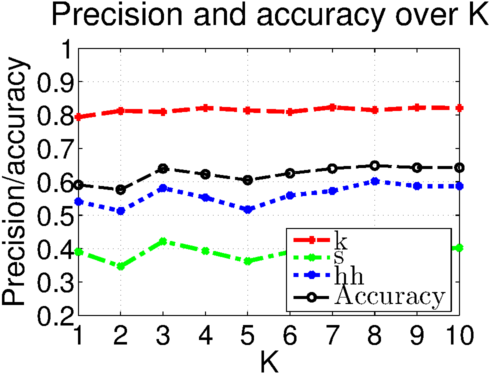
\includegraphics[width=0.3\textwidth]{tex/appendices/test/sskew2010_P.png}
%			\centering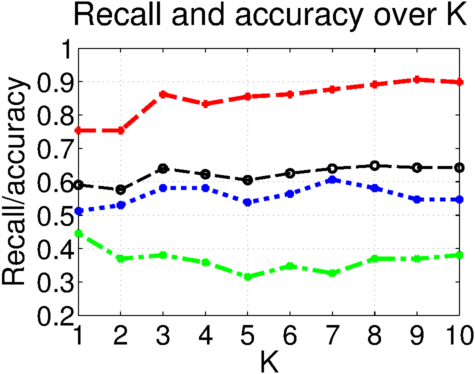
\includegraphics[width=0.3\textwidth]{tex/appendices/test/sskew2010_R.png}
%			
%			\caption{Plots over K for Spectral Skew with 20ms windows and 10ms window skips}
%		\end{figure}
%		
%		\begin{figure}
%			\centering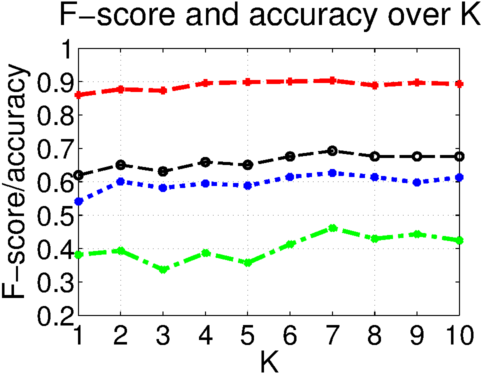
\includegraphics[width=0.3\textwidth]{tex/appendices/test/sskew105FP.png}
%			\centering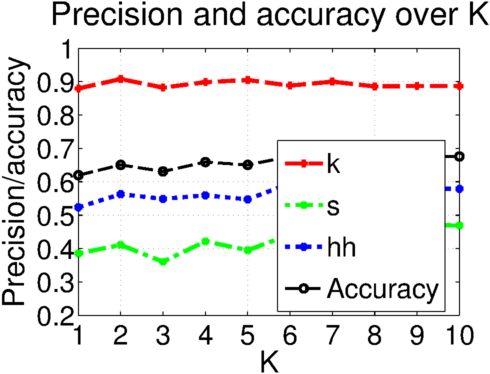
\includegraphics[width=0.3\textwidth]{tex/appendices/test/sskew105_P.png}
%			\centering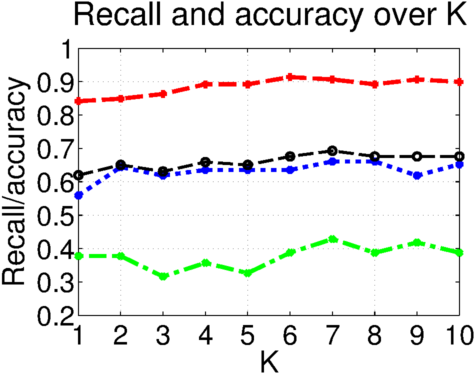
\includegraphics[width=0.3\textwidth]{tex/appendices/test/sskew105_R.png}
%				
%				\caption{Plots over K for Spectral Skew with 10ms windows and 5ms window skips}
%		\end{figure}
%		\begin{figure}
%			\centering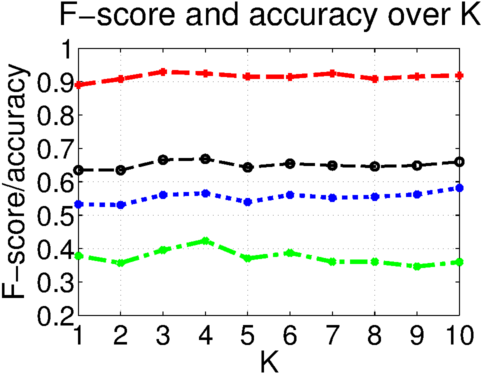
\includegraphics[width=0.3\textwidth]{tex/appendices/test/sskew52FP.png}
%			\centering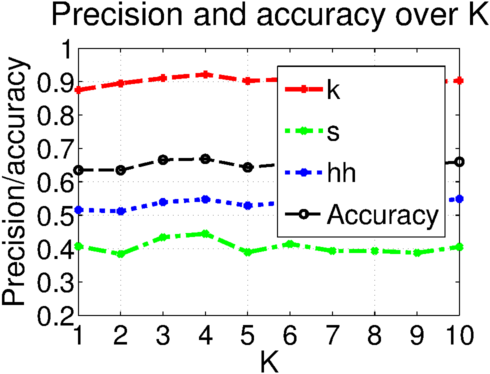
\includegraphics[width=0.3\textwidth]{tex/appendices/test/sskew52_P.png}
%			\centering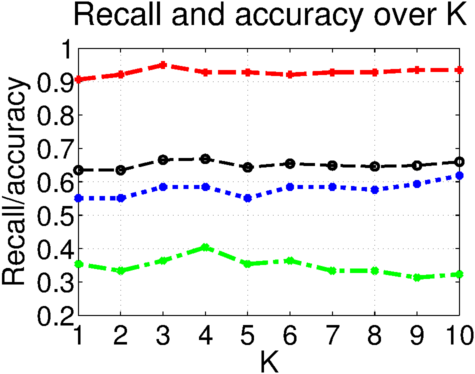
\includegraphics[width=0.3\textwidth]{tex/appendices/test/sskew52_R.png}
%				
%				\caption{Plots over K for Spectral Skew with 5ms windows and 2ms window skips}
%		\end{figure}\clearpage
%		
%		\begin{table}
%			\begin{subtable}[h]{0.45\textwidth}
%				\centering
%				\begin{tabular}{|c|c|c|c"c|}
%					 \cline{2-5}
%					 \multicolumn{1}{c|}{} & \textbf{k}  & \textbf{s}  & \textbf{hh}  & Prec.\\ \hline
%					 \textbf{k} & \textcolor{red}{0.942} & 0.031 & 0.008 & 0.970\\ \hline
%					 \textbf{s} & 0.058 & \textcolor{red}{0.786} & 0.288 & 0.647\\ \hline
%					 \textbf{hh} & 0.058 & 0.184 & \textcolor{red}{0.703} & 0.822\\ \Xhline{2\arrayrulewidth}
%					  F & 0.956 & 0.710 & 0.758 & \textcolor{blue}{0.820}\\ \hline
%				\end{tabular}
%				\caption{$wSize=10ms, wSkip=5ms, K=7$}
%				\label{table:eval:skewBest}
%			\end{subtable}
%			\hfill
%			\begin{subtable}[h]{0.45\textwidth}
%				\centering
%				\begin{tabular}{|c|c|c|c"c|}
%					\cline{2-5}
%					 \multicolumn{1}{c|}{} & \textbf{k}  & \textbf{s}  & \textbf{hh}  & Prec.\\ \hline
%					 \textbf{k} & \textcolor{red}{0.964} & 0.081 & 0.008 & 0.937\\ \hline
%					 \textbf{s} & 0.036 & \textcolor{red}{0.768} & 0.280 & 0.667\\ \hline
%					 \textbf{hh} & 0.036 & 0.152 & \textcolor{red}{0.712} & 0.848\\ \Xhline{2\arrayrulewidth}
%					 F & 0.950 & 0.714 & 0.774 & \textcolor{blue}{0.826}\\ \hline
%				\end{tabular}
%				\caption{$wSize=5ms, wSkip=2ms, K=7$}
%				\label{table:eval:skewKicker}
%			\end{subtable}
%			\hfill
%			\begin{subtable}[h]{0.45\textwidth}
%				\centering
%				\begin{tabular}{|c|c|c|c"c|}
%					\cline{2-5}
%					 \multicolumn{1}{c|}{} & \textbf{k}  & \textbf{s}  & \textbf{hh}  & Prec.\\ \hline
%					 \textbf{k} & \textcolor{red}{0.920} & 0.163 & 0.009 & 0.888\\ \hline
%					 \textbf{s} & 0.072 & \textcolor{red}{0.446} & 0.239 & 0.519\\ \hline
%					 \textbf{hh} & 0.072 & 0.391 & \textcolor{red}{0.752} & 0.704\\ \Xhline{2\arrayrulewidth}
%					 F & 0.904 & 0.480 & 0.727 & \textcolor{blue}{0.738}\\ \hline
%				\end{tabular}
%				\caption{$wSize=20ms, wSkip=10ms, K=2$}
%				\label{table:eval:skewWorst}
%			\end{subtable}
%			\caption{Measures over K using Spectral Skewness}
%		\end{table}
		

		The most accurate result using Spectral Skew was 82\%, was $K=7$ with 10ms window size and 5ms window skip, as shown in appendix \ref{app:SS:7:best}. Some other tests was more precise on kicks (e.g. Spectral Skew with 5ms window and 2ms window skip, with $K=7$, see \ref{app:SS:7:kickbest}). The least accurate result was $K=2$, using 20ms window size, 10ms window skip (see appendix \ref{app:SS:2:worst}). $X^2$-test did not show any significant results.
	
	%
	% SF
	%
	\subsection{Spectral Flux}
		
%		\begin{figure}
%		
%			\label{figJitter}
%			\centering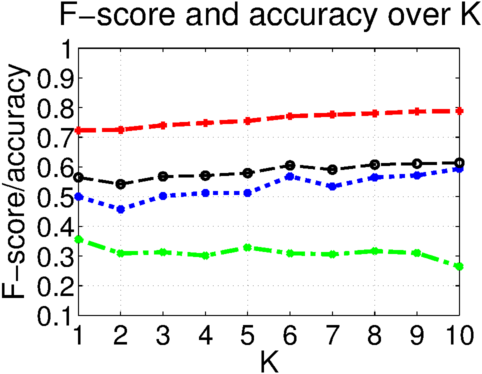
\includegraphics[width=0.3\textwidth]{tex/appendices/test/sflux2010FP.png}
%			\centering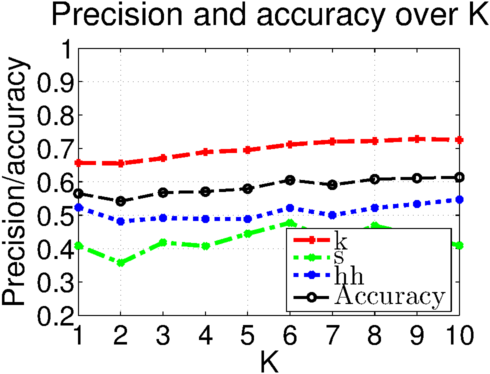
\includegraphics[width=0.3\textwidth]{tex/appendices/test/sflux2010_P.png}
%			\centering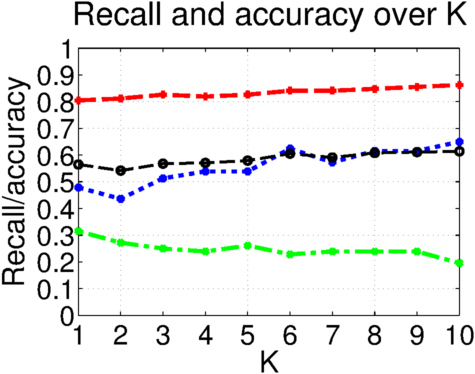
\includegraphics[width=0.3\textwidth]{tex/appendices/test/sflux2010_R.png}
%			
%			\caption{Plots over K for Spectral Flux with 20ms windows and 10ms window skips}
%		\end{figure}
%		\begin{figure}
%		
%		
%			\centering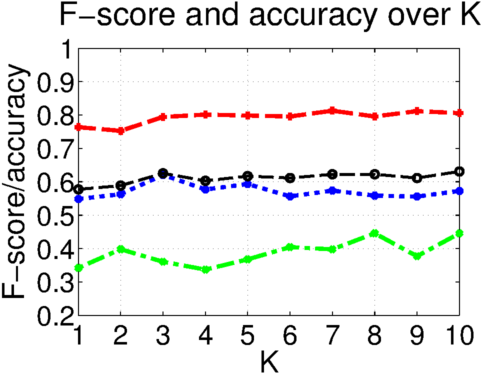
\includegraphics[width=0.3\textwidth]{tex/appendices/test/sflux105FP.png}
%			\centering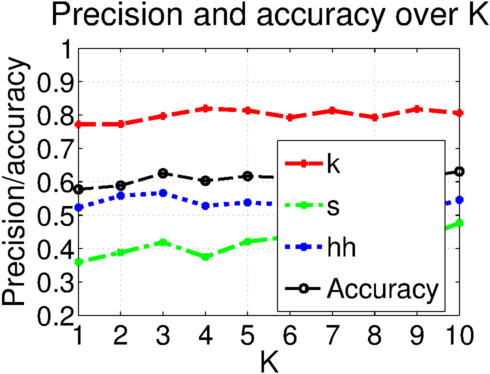
\includegraphics[width=0.3\textwidth]{tex/appendices/test/sflux105_P.png}
%			\centering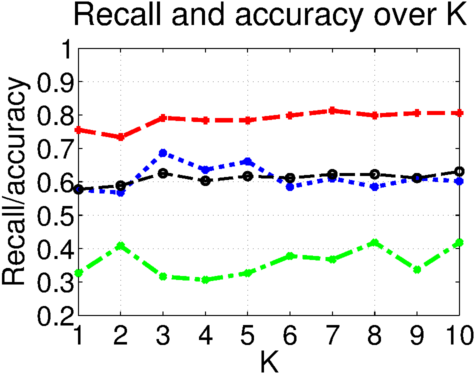
\includegraphics[width=0.3\textwidth]{tex/appendices/test/sflux105_R.png}
%				
%				\caption{Plots over K for Spectral Flux with 10ms windows and 5ms window skips}
%		\end{figure}
%		\begin{figure}
%		
%		
%			\centering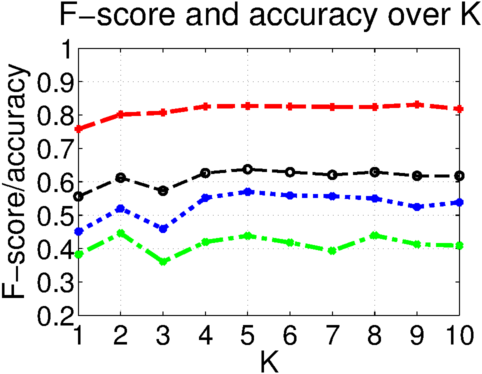
\includegraphics[width=0.3\textwidth]{tex/appendices/test/sflux52FP.png}
%			\centering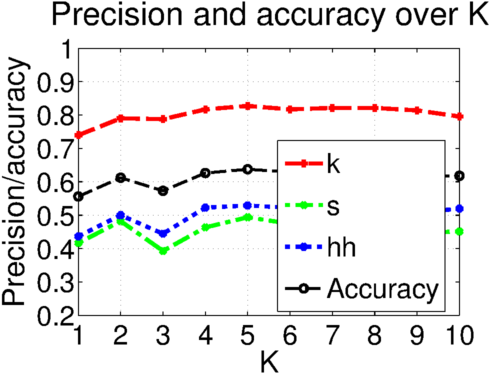
\includegraphics[width=0.3\textwidth]{tex/appendices/test/sflux52_P.png}
%			\centering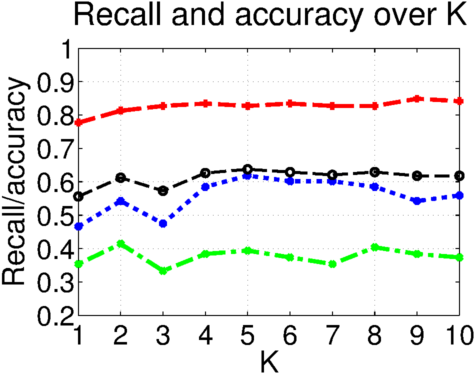
\includegraphics[width=0.3\textwidth]{tex/appendices/test/sflux52_R.png}
%				
%				\caption{Plots over K for Spectral Flux with 5ms windows and 2ms window skips}
%		\end{figure}
%		
%		\begin{table}
%			\begin{subtable}[h]{0.45\textwidth}
%				\centering
%				\begin{tabular}{|c|c|c|c"c|}
%					\cline{2-5}
%					 \multicolumn{1}{c|}{} & \textbf{k}  & \textbf{s}  & \textbf{hh}  & Prec.\\ \hline
%					 \textbf{k} & \textcolor{red}{0.827} & 0.121 & 0.102 & 0.827\\ \hline
%					 \textbf{s} & 0.050 & \textcolor{red}{0.394} & 0.280 & 0.494\\ \hline
%					 \textbf{hh} & 0.050 & 0.485 & \textcolor{red}{0.619} & 0.529\\ \Xhline{2\arrayrulewidth}
%					 F & 0.827 & 0.438 & 0.570 & \textcolor{blue}{0.638}\\ \hline
%				\end{tabular}
%				\caption{$wSize=5ms, wSkip=2ms, K=5$}
%				\label{table:eval:fluxBest}
%			\end{subtable}
%			\hfill
%			\begin{subtable}[h]{0.45\textwidth}
%				\centering
%				\begin{tabular}{|c|c|c|c"c|}
%					\cline{2-5}
%					 \multicolumn{1}{c|}{} & \textbf{k}  & \textbf{s}  & \textbf{hh}  & Prec.\\ \hline
%					 \textbf{k} & \textcolor{red}{0.812} & 0.293 & 0.274 & 0.655\\ \hline
%					 \textbf{s} & 0.080 & \textcolor{red}{0.272} & 0.291 & 0.357\\ \hline
%					 \textbf{hh} & 0.080 & 0.435 & \textcolor{red}{0.436} & 0.481\\ \Xhline{2\arrayrulewidth}
%					 F & 0.725 & 0.309 & 0.457 & \textcolor{blue}{0.542}\\ \hline
%				\end{tabular}
%				\caption{$wSize=20ms, wSkip=10ms, K=2$}
%				\label{table:eval:fluxWorst}
%			\end{subtable}
%			
%			\caption{Measures over K using Spectral Flux}
%		\end{table}
		
		The most accurate results with the Spectral Flux feature vector, was with 5ms window size, 2ms window skip, and $K=5$ (appendix \ref{app:SF:5:best}), however several test configurations using other feature parameters, show better precision for the highhat. The worst in terms of accuracy is the Spectral Flux using 20ms windows and 10ms window skips, with $K=2$, see appendix \ref{app:SF:2:worst}.	$X^2$ showed no significant results.

 \subsection{Recapitulating the results}
 To recap slightly from the previous chapter: Overall, the highest accuracy was obtained using MFCC over a window of 5ms with a skip of 2ms, with $k=7$ and $k=8$. Our $X^2$ tests did not show a significant difference even once, so our null-hypothesis stands true. This was unexpected, although some probabilities come very close, so perhaps the result might look different in future tests (with slightly different data due to randomization).

\bibliography{sources}
\bibliographystyle{apalike}

\begin{appendices}
\chapter{Project Results}

\section{Results}
\label{app:res}
\subsection{RMS}
	\label{app:res:rms}
	\begin{figure}

	\centering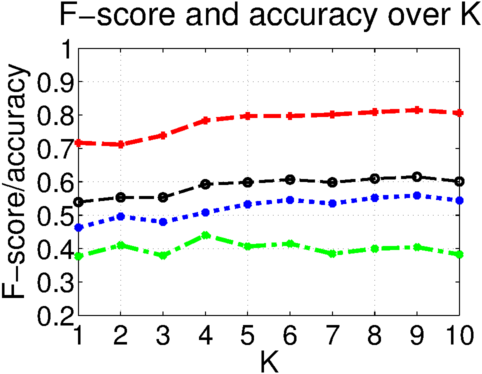
\includegraphics[width=0.3\textwidth]{tex/appendices/test/rms11FP.png}
	\centering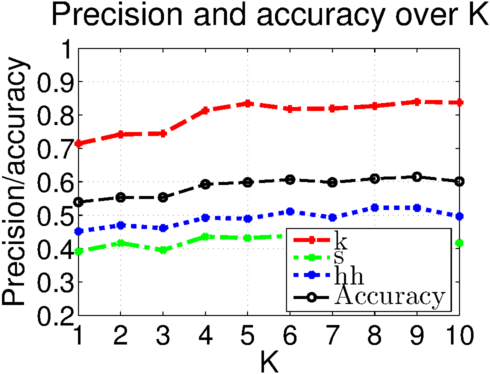
\includegraphics[width=0.3\textwidth]{tex/appendices/test/rms11_P.png}
	\centering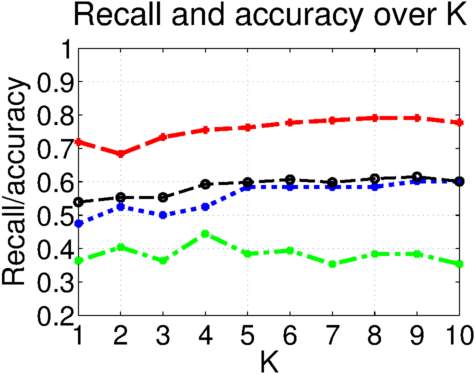
\includegraphics[width=0.3\textwidth]{tex/appendices/test/rms11_R.png}
	
	\caption{Plots over K for Root Mean Square}
\end{figure}


\begin{table}
\begin{subtable}[tbp]{0.45\textwidth}
\centering


\begin{tabular}{|c|c|c|c"c|}
\cline{2-5}
 \multicolumn{1}{c|}{} & \textbf{k}  & \textbf{s}  & \textbf{hh}  & Prec.\\ \hline
 \textbf{k} & \textcolor{red}{0.719} & 0.212 & 0.161 & 0.714\\ \hline
 \textbf{s} & 0.094 & \textcolor{red}{0.364} & 0.364 & 0.391\\ \hline
 \textbf{hh} & 0.094 & 0.424 & \textcolor{red}{0.475} & 0.452\\ \Xhline{2\arrayrulewidth}
 F & 0.717 & 0.377 & 0.463 & \textcolor{blue}{0.539}\\ \hline
\end{tabular}
\caption{$K=1$}
\label{app:RMS:1:worst}
\end{subtable}
\hfill


\begin{subtable}[tbp]{0.45\textwidth}
\centering
\begin{tabular}{|c|c|c|c"c|}
\cline{2-5}
 \multicolumn{1}{c|}{} & \textbf{k}  & \textbf{s}  & \textbf{hh}  & Prec.\\ \hline
 \textbf{k} & \textcolor{red}{0.683} & 0.172 & 0.136 & 0.742\\ \hline
 \textbf{s} & 0.115 & \textcolor{red}{0.404} & 0.339 & 0.417\\ \hline
 \textbf{hh} & 0.115 & 0.424 & \textcolor{red}{0.525} & 0.470\\ \Xhline{2\arrayrulewidth}
 F & 0.712 & 0.410 & 0.496 & \textcolor{blue}{0.553}\\ \hline
\end{tabular}
\caption{$K=2$}
\end{subtable}
\hfill
\begin{subtable}[tbp]{0.45\textwidth}
\centering


\begin{tabular}{|c|c|c|c"c|}
\cline{2-5}
 \multicolumn{1}{c|}{} & \textbf{k}  & \textbf{s}  & \textbf{hh}  & Prec.\\ \hline
 \textbf{k} & \textcolor{red}{0.734} & 0.192 & 0.136 & 0.745\\ \hline
 \textbf{s} & 0.086 & \textcolor{red}{0.364} & 0.364 & 0.396\\ \hline
 \textbf{hh} & 0.086 & 0.444 & \textcolor{red}{0.500} & 0.461\\ \Xhline{2\arrayrulewidth}
 F & 0.739 & 0.379 & 0.480 & \textcolor{blue}{0.553}\\ \hline
\end{tabular}
\caption{$K=3$}
\end{subtable}
\hfill


\begin{subtable}[tbp]{0.45\textwidth}
\centering
\begin{tabular}{|c|c|c|c"c|}
\cline{2-5}
 \multicolumn{1}{c|}{} & \textbf{k}  & \textbf{s}  & \textbf{hh}  & Prec.\\ \hline
 \textbf{k} & \textcolor{red}{0.755} & 0.121 & 0.102 & 0.814\\ \hline
 \textbf{s} & 0.094 & \textcolor{red}{0.444} & 0.373 & 0.436\\ \hline
 \textbf{hh} & 0.094 & 0.434 & \textcolor{red}{0.525} & 0.492\\ \Xhline{2\arrayrulewidth}
 F & 0.784 & 0.440 & 0.508 & \textcolor{blue}{0.593}\\ \hline
\end{tabular}
\caption{$K=4$}
\end{subtable}
\hfill


\begin{subtable}[tbp]{0.45\textwidth}
\centering
\begin{tabular}{|c|c|c|c"c|}
\cline{2-5}
 \multicolumn{1}{c|}{} & \textbf{k}  & \textbf{s}  & \textbf{hh}  & Prec.\\ \hline
 \textbf{k} & \textcolor{red}{0.763} & 0.111 & 0.085 & 0.835\\ \hline
 \textbf{s} & 0.079 & \textcolor{red}{0.384} & 0.331 & 0.432\\ \hline
 \textbf{hh} & 0.079 & 0.505 & \textcolor{red}{0.585} & 0.489\\ \Xhline{2\arrayrulewidth}
 F & 0.797 & 0.406 & 0.533 & \textcolor{blue}{0.598}\\ \hline
\end{tabular}
\caption{$K=5$}
\end{subtable}
\hfill


\begin{subtable}[tbp]{0.45\textwidth}
\centering
\begin{tabular}{|c|c|c|c"c|}
\cline{2-5}
 \multicolumn{1}{c|}{} & \textbf{k}  & \textbf{s}  & \textbf{hh}  & Prec.\\ \hline
 \textbf{k} & \textcolor{red}{0.777} & 0.121 & 0.102 & 0.818\\ \hline
 \textbf{s} & 0.094 & \textcolor{red}{0.394} & 0.314 & 0.438\\ \hline
 \textbf{hh} & 0.094 & 0.485 & \textcolor{red}{0.585} & 0.511\\ \Xhline{2\arrayrulewidth}
 F & 0.797 & 0.415 & 0.545 & \textcolor{blue}{0.607}\\ \hline
\end{tabular}
\caption{$K=6$}
\label{app:rms:k6}
\end{subtable}
\hfill


\begin{subtable}[tbp]{0.45\textwidth}
\centering
\begin{tabular}{|c|c|c|c"c|}
\cline{2-5}
 \multicolumn{1}{c|}{} & \textbf{k}  & \textbf{s}  & \textbf{hh}  & Prec.\\ \hline
 \textbf{k} & \textcolor{red}{0.784} & 0.131 & 0.093 & 0.820\\ \hline
 \textbf{s} & 0.072 & \textcolor{red}{0.354} & 0.322 & 0.422\\ \hline
 \textbf{hh} & 0.072 & 0.515 & \textcolor{red}{0.585} & 0.493\\ \Xhline{2\arrayrulewidth}
 F & 0.801 & 0.385 & 0.535 & \textcolor{blue}{0.598}\\ \hline
\end{tabular}
\caption{$K=7$}
\end{subtable}
\hfill


\begin{subtable}[tbp]{0.45\textwidth}
\centering
\begin{tabular}{|c|c|c|c"c|}
\cline{2-5}
 \multicolumn{1}{c|}{} & \textbf{k}  & \textbf{s}  & \textbf{hh}  & Prec.\\ \hline
 \textbf{k} & \textcolor{red}{0.791} & 0.141 & 0.076 & 0.827\\ \hline
 \textbf{s} & 0.094 & \textcolor{red}{0.384} & 0.339 & 0.418\\ \hline
 \textbf{hh} & 0.094 & 0.475 & \textcolor{red}{0.585} & 0.523\\ \Xhline{2\arrayrulewidth}
 F & 0.809 & 0.400 & 0.552 & \textcolor{blue}{0.610}\\ \hline
\end{tabular}
\caption{$K=8$}
\label{app:rms:k8}
\end{subtable}
\hfill
\begin{subtable}[tbp]{0.45\textwidth}
\centering
\begin{tabular}{|c|c|c|c"c|}
\cline{2-5}
 \multicolumn{1}{c|}{} & \textbf{k}  & \textbf{s}  & \textbf{hh}  & Prec.\\ \hline
 \textbf{k} & \textcolor{red}{0.791} & 0.141 & 0.059 & 0.840\\ \hline
 \textbf{s} & 0.079 & \textcolor{red}{0.384} & 0.339 & 0.427\\ \hline
 \textbf{hh} & 0.079 & 0.475 & \textcolor{red}{0.602} & 0.522\\ \Xhline{2\arrayrulewidth}
 F & 0.815 & 0.404 & 0.559 & \textcolor{blue}{0.615}\\ \hline
\end{tabular}
\caption{$K=9$}
\label{app:RMS:9}
\end{subtable}
\hfill


\begin{subtable}[tbp]{0.45\textwidth}
\centering
\begin{tabular}{|c|c|c|c"c|}
\cline{2-5}
 \multicolumn{1}{c|}{} & \textbf{k}  & \textbf{s}  & \textbf{hh}  & Prec.\\ \hline
 \textbf{k} & \textcolor{red}{0.777} & 0.121 & 0.076 & 0.837\\ \hline
 \textbf{s} & 0.079 & \textcolor{red}{0.354} & 0.322 & 0.417\\ \hline
 \textbf{hh} & 0.079 & 0.525 & \textcolor{red}{0.602} & 0.497\\ \Xhline{2\arrayrulewidth}
 F & 0.806 & 0.383 & 0.544 & \textcolor{blue}{0.601}\\ \hline
\end{tabular}
\caption{$K=10$}
\end{subtable}
\hfill


\caption{tcrms11}
\label{tlrms11}

\end{table}\clearpage


\begin{table}


\begin{subtable}[h]{0.45\textwidth}
\centering
 \scalebox{0.8}{
\begin{tabular}{|c|c|c|c|}\hline
 $K_1$ & $K_2$ & $X^2$ & p\\ \hline
 1 & 2 & 54.000 & 0.25605\\ \hline 
 1 & 3 & 72.000 & 0.23040\\ \hline 
 1 & 4 & 54.000 & 0.25605\\ \hline 
 1 & 5 & 63.000 & 0.24255\\ \hline 
 1 & 6 & 63.000 & 0.24255\\ \hline 
 1 & 7 & 72.000 & 0.23040\\ \hline 
 1 & 8 & 72.000 & 0.23040\\ \hline 
 1 & 9 & 72.000 & 0.23040\\ \hline 
 1 & 10 & 72.000 & 0.23040\\ \hline 
 2 & 3 & 54.000 & 0.25605\\ \hline 
 2 & 4 & 47.250 & 0.09945\\ \hline 
 2 & 5 & 47.250 & 0.26685\\ \hline 
 2 & 6 & 47.250 & 0.26685\\ \hline 
 2 & 7 & 54.000 & 0.25605\\ \hline 
 2 & 8 & 54.000 & 0.25605\\ \hline 
 2 & 9 & 54.000 & 0.25605\\ \hline 
 2 & 10 & 54.000 & 0.25605\\ \hline 
 3 & 4 & 54.000 & 0.25605\\ \hline 
 3 & 5 & 63.000 & 0.24255\\ \hline 
 3 & 6 & 63.000 & 0.24255\\ \hline 
 3 & 7 & 72.000 & 0.23040\\ \hline 
 3 & 8 & 72.000 & 0.23040\\ \hline 
 3 & 9 & 72.000 & 0.23040\\ \hline 
 3 & 10 & 72.000 & 0.23040\\ \hline 
 4 & 5 & 47.250 & 0.26685\\ \hline 
 4 & 6 & 54.000 & 0.00225\\ \hline 
 4 & 7 & 54.000 & 0.25605\\ \hline 
 4 & 8 & 54.000 & 0.25605\\ \hline 
 4 & 9 & 54.000 & 0.25605\\ \hline 
 4 & 10 & 54.000 & 0.25605\\ \hline 
 5 & 6 & 56.250 & 0.022185\\ \hline 
 5 & 7 & 63.000 & 0.24255\\ \hline 
 5 & 8 & 63.000 & 0.24255\\ \hline 
 5 & 9 & 63.000 & 0.24255\\ \hline 
 5 & 10 & 63.000 & 0.24255\\ \hline 
 6 & 7 & 63.000 & 0.24255\\ \hline 
 6 & 8 & 63.000 & 0.24255\\ \hline 
 6 & 9 & 63.000 & 0.24255\\ \hline 
 6 & 10 & 63.000 & 0.24255\\ \hline 
 7 & 8 & 72.000 & 0.23040\\ \hline 
 7 & 9 & 72.000 & 0.23040\\ \hline 
 7 & 10 & 72.000 & 0.23040\\ \hline 
 8 & 9 & 72.000 & 0.23040\\ \hline 
 8 & 10 & 72.000 & 0.23040\\ \hline 
 9 & 10 & 72.000 & 0.23040\\ \hline 

\end{tabular}
}\caption{xcrms11}
 \label{xlrms11}
\end{subtable}

\begin{subtable}[h]{0.45\textwidth}
\centering
\begin{tabular}{|c|c|c|}
\hline
Class & Amount & Percent\\ \hline
k & 326 & 39.14\\ \hline
s & 231 & 27.73\\ \hline
hh & 276 & 33.13\\ \hline
\end{tabular}
\caption{Training dataset}
\end{subtable}
\hfill
\begin{subtable}[h]{0.45\textwidth}
\centering
\begin{tabular}{|c|c|c|}
\hline
Class & Amount & Percent\\ \hline
k & 139 & 39.04\\ \hline
s & 99 & 27.81\\ \hline
hh & 118 & 33.15\\ \hline
\end{tabular}
\caption{Testing dataset}
\end{subtable}
\hfill


\caption{dcrms11}

\label{dlrms11}
\end{table}

\subsection{ZCR}
	\label{cmon}
	\begin{figure}
	\centering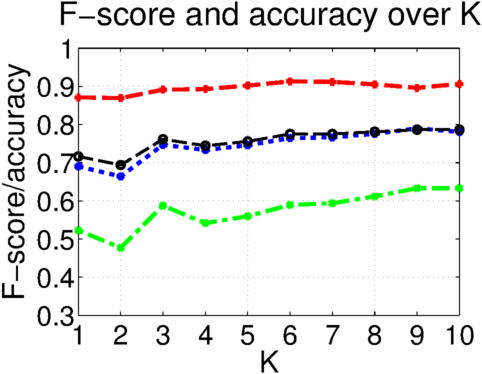
\includegraphics[width=0.3\textwidth]{tex/appendices/test/zcr11FP.png}
	\centering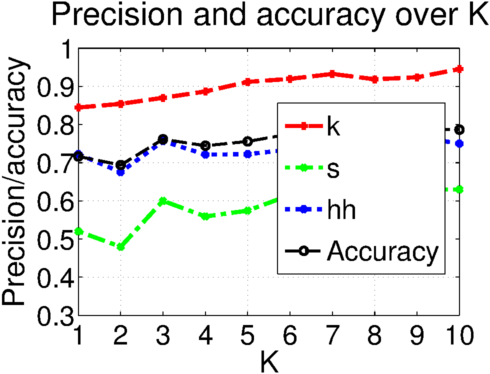
\includegraphics[width=0.3\textwidth]{tex/appendices/test/zcr11_P.png}
	\centering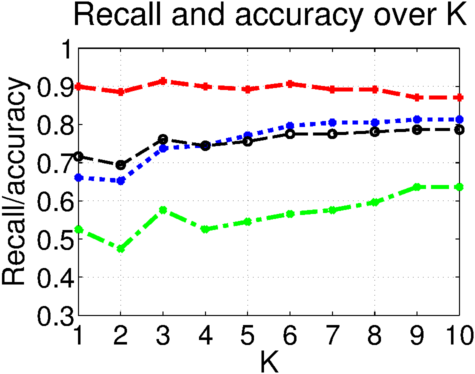
\includegraphics[width=0.3\textwidth]{tex/appendices/test/zcr11_R.png}
	\caption{Plots over K for Zero Crossing Rate}
\end{figure}


\begin{table}
\begin{subtable}[tbp]{0.45\textwidth}
\centering
\begin{tabular}{|c|c|c|c"c|}
\cline{2-5}
 \multicolumn{1}{c|}{} & \textbf{k}  & \textbf{s}  & \textbf{hh}  & Prec.\\ \hline
 \textbf{k} & \textcolor{red}{0.899} & 0.172 & 0.051 & 0.845\\ \hline
 \textbf{s} & 0.101 & \textcolor{red}{0.525} & 0.288 & 0.520\\ \hline
 \textbf{hh} & 0.101 & 0.303 & \textcolor{red}{0.661} & 0.722\\ \Xhline{2\arrayrulewidth}
 F & 0.871 & 0.523 & 0.690 & \textcolor{blue}{0.716}\\ \hline
\end{tabular}
\caption{$K=1$}
\end{subtable}
\hfill
\begin{subtable}[tbp]{0.45\textwidth}
\centering
\begin{tabular}{|c|c|c|c"c|}
\cline{2-5}
 \multicolumn{1}{c|}{} & \textbf{k}  & \textbf{s}  & \textbf{hh}  & Prec.\\ \hline
 \textbf{k} & \textcolor{red}{0.885} & 0.162 & 0.042 & 0.854\\ \hline
 \textbf{s} & 0.108 & \textcolor{red}{0.475} & 0.305 & 0.480\\ \hline
 \textbf{hh} & 0.108 & 0.364 & \textcolor{red}{0.653} & 0.675\\ \Xhline{2\arrayrulewidth}
 F & 0.869 & 0.477 & 0.664 & \textcolor{blue}{0.694}\\ \hline
\end{tabular}
\caption{$K=2$}
\label{app-ZCR-Worst}
\end{subtable}
\hfill
\begin{subtable}[tbp]{0.45\textwidth}
\centering
\begin{tabular}{|c|c|c|c"c|}
\cline{2-5}
 \multicolumn{1}{c|}{} & \textbf{k}  & \textbf{s}  & \textbf{hh}  & Prec.\\ \hline
 \textbf{k} & \textcolor{red}{0.914} & 0.141 & 0.042 & 0.870\\ \hline
 \textbf{s} & 0.086 & \textcolor{red}{0.576} & 0.220 & 0.600\\ \hline
 \textbf{hh} & 0.086 & 0.283 & \textcolor{red}{0.737} & 0.757\\ \Xhline{2\arrayrulewidth}
 F & 0.891 & 0.588 & 0.747 & \textcolor{blue}{0.761}\\ \hline
\end{tabular}
\caption{$K=3$}
\end{subtable}
\hfill
\begin{subtable}[tbp]{0.45\textwidth}
\centering
\begin{tabular}{|c|c|c|c"c|}
\cline{2-5}
 \multicolumn{1}{c|}{} & \textbf{k}  & \textbf{s}  & \textbf{hh}  & Prec.\\ \hline
 \textbf{k} & \textcolor{red}{0.899} & 0.131 & 0.025 & 0.887\\ \hline
 \textbf{s} & 0.101 & \textcolor{red}{0.525} & 0.229 & 0.559\\ \hline
 \textbf{hh} & 0.101 & 0.343 & \textcolor{red}{0.746} & 0.721\\ \Xhline{2\arrayrulewidth}
 F & 0.893 & 0.542 & 0.733 & \textcolor{blue}{0.744}\\ \hline
\end{tabular}
\caption{$K=4$}
\end{subtable}
\hfill
\begin{subtable}[tbp]{0.45\textwidth}
\centering
\begin{tabular}{|c|c|c|c"c|}
\cline{2-5}
 \multicolumn{1}{c|}{} & \textbf{k}  & \textbf{s}  & \textbf{hh}  & Prec.\\ \hline
 \textbf{k} & \textcolor{red}{0.892} & 0.101 & 0.017 & 0.912\\ \hline
 \textbf{s} & 0.108 & \textcolor{red}{0.545} & 0.212 & 0.574\\ \hline
 \textbf{hh} & 0.108 & 0.354 & \textcolor{red}{0.771} & 0.722\\ \Xhline{2\arrayrulewidth}
 F & 0.902 & 0.560 & 0.746 & \textcolor{blue}{0.756}\\ \hline
\end{tabular}
\caption{$K=5$}
\end{subtable}
\hfill
\begin{subtable}[tbp]{0.45\textwidth}
\centering
\begin{tabular}{|c|c|c|c"c|}
\cline{2-5}
 \multicolumn{1}{c|}{} & \textbf{k}  & \textbf{s}  & \textbf{hh}  & Prec.\\ \hline
 \textbf{k} & \textcolor{red}{0.906} & 0.091 & 0.017 & 0.920\\ \hline
 \textbf{s} & 0.094 & \textcolor{red}{0.566} & 0.186 & 0.615\\ \hline
 \textbf{hh} & 0.094 & 0.343 & \textcolor{red}{0.797} & 0.734\\ \Xhline{2\arrayrulewidth}
 F & 0.913 & 0.589 & 0.764 & \textcolor{blue}{0.775}\\ \hline
\end{tabular}
\caption{$K=6$}
\end{subtable}
\hfill
\begin{subtable}[tbp]{0.45\textwidth}
\centering
\begin{tabular}{|c|c|c|c"c|}
\cline{2-5}
 \multicolumn{1}{c|}{} & \textbf{k}  & \textbf{s}  & \textbf{hh}  & Prec.\\ \hline
 \textbf{k} & \textcolor{red}{0.892} & 0.071 & 0.017 & 0.932\\ \hline
 \textbf{s} & 0.108 & \textcolor{red}{0.576} & 0.178 & 0.613\\ \hline
 \textbf{hh} & 0.108 & 0.354 & \textcolor{red}{0.805} & 0.731\\ \Xhline{2\arrayrulewidth}
 F & 0.912 & 0.594 & 0.766 & \textcolor{blue}{0.775}\\ \hline
\end{tabular}
\caption{$K=7$}
\end{subtable}
\hfill
\begin{subtable}[tbp]{0.45\textwidth}
\centering
\begin{tabular}{|c|c|c|c"c|}
\cline{2-5}
 \multicolumn{1}{c|}{} & \textbf{k}  & \textbf{s}  & \textbf{hh}  & Prec.\\ \hline
 \textbf{k} & \textcolor{red}{0.892} & 0.091 & 0.017 & 0.919\\ \hline
 \textbf{s} & 0.101 & \textcolor{red}{0.596} & 0.178 & 0.628\\ \hline
 \textbf{hh} & 0.101 & 0.313 & \textcolor{red}{0.805} & 0.748\\ \Xhline{2\arrayrulewidth}
 F & 0.905 & 0.611 & 0.776 & \textcolor{blue}{0.781}\\ \hline
\end{tabular}
\caption{$K=8$}
\end{subtable}
\hfill
\begin{subtable}[tbp]{0.45\textwidth}
\centering
\begin{tabular}{|c|c|c|c"c|}
\cline{2-5}
 \multicolumn{1}{c|}{} & \textbf{k}  & \textbf{s}  & \textbf{hh}  & Prec.\\ \hline
 \textbf{k} & \textcolor{red}{0.871} & 0.081 & 0.017 & 0.924\\ \hline
 \textbf{s} & 0.122 & \textcolor{red}{0.636} & 0.169 & 0.630\\ \hline
 \textbf{hh} & 0.122 & 0.283 & \textcolor{red}{0.814} & 0.768\\ \Xhline{2\arrayrulewidth}
 F & 0.896 & 0.633 & 0.790 & \textcolor{blue}{0.787}\\ \hline
\end{tabular}
\caption{$K=9$}
\label{app:zcr:best}
\end{subtable}
\hfill
\begin{subtable}[tbp]{0.45\textwidth}
\centering
\begin{tabular}{|c|c|c|c"c|}
\cline{2-5}
 \multicolumn{1}{c|}{} & \textbf{k}  & \textbf{s}  & \textbf{hh}  & Prec.\\ \hline
 \textbf{k} & \textcolor{red}{0.871} & 0.051 & 0.017 & 0.945\\ \hline
 \textbf{s} & 0.122 & \textcolor{red}{0.636} & 0.169 & 0.630\\ \hline
 \textbf{hh} & 0.122 & 0.313 & \textcolor{red}{0.814} & 0.750\\ \Xhline{2\arrayrulewidth}
 F & 0.906 & 0.633 & 0.780 & \textcolor{blue}{0.787}\\ \hline
\end{tabular}
\caption{$K=10$}
\label{app:zcr:best2}
\end{subtable}
\hfill

\caption{tczcr11}

\label{tlzcr11}

\end{table}\clearpage


\begin{table}

\begin{subtable}[tbp]{0.4\textwidth}
\centering
 
\begin{tabular}{|c|c|c|c|}\hline
 $K_1$ & $K_2$ & $X^2$ & p\\ \hline
 1 & 2 & 63.000 & 0.24255\\ \hline 
 1 & 3 & 72.000 & 0.2304\\ \hline 
 1 & 4 & 72.000 & 0.2304\\ \hline 
 1 & 5 & 72.000 & 0.2304\\ \hline 
 1 & 6 & 72.000 & 0.2304\\ \hline 
 1 & 7 & 72.000 & 0.2304\\ \hline 
 1 & 8 & 72.000 & 0.2304\\ \hline 
 1 & 9 & 72.000 & 0.2304\\ \hline 
 1 & 10 & 72.000 & 0.2304\\ \hline 
 2 & 3 & 63.000 & 0.24255\\ \hline 
 2 & 4 & 63.000 & 0.24255\\ \hline 
 2 & 5 & 63.000 & 0.24255\\ \hline 
 2 & 6 & 63.000 & 0.24255\\ \hline 
 2 & 7 & 63.000 & 0.24255\\ \hline 
 2 & 8 & 63.000 & 0.24255\\ \hline 
 2 & 9 & 63.000 & 0.24255\\ \hline 
 2 & 10 & 63.000 & 0.24255\\ \hline 
 3 & 4 & 72.000 & 0.2304\\ \hline 
 3 & 5 & 72.000 & 0.2304\\ \hline 
 3 & 6 & 72.000 & 0.2304\\ \hline 
 3 & 7 & 72.000 & 0.2304\\ \hline 
 3 & 8 & 72.000 & 0.2304\\ \hline 
 3 & 9 & 72.000 & 0.2304\\ \hline 
 3 & 10 & 72.000 & 0.2304\\ \hline 
 4 & 5 & 72.000 & 0.2304\\ \hline 
 4 & 6 & 72.000 & 0.2304\\ \hline 
 4 & 7 & 72.000 & 0.2304\\ \hline 
 4 & 8 & 72.000 & 0.2304\\ \hline 
 4 & 9 & 72.000 & 0.2304\\ \hline 
 4 & 10 & 72.000 & 0.2304\\ \hline 
 5 & 6 & 72.000 & 0.2304\\ \hline 
 5 & 7 & 72.000 & 0.2304\\ \hline 
 5 & 8 & 72.000 & 0.2304\\ \hline 
 5 & 9 & 72.000 & 0.2304\\ \hline 
 5 & 10 & 72.000 & 0.2304\\ \hline 
 6 & 7 & 72.000 & 0.2304\\ \hline 
 6 & 8 & 72.000 & 0.2304\\ \hline 
 6 & 9 & 72.000 & 0.2304\\ \hline 
 6 & 10 & 72.000 & 0.2304\\ \hline 
 7 & 8 & 72.000 & 0.2304\\ \hline 
 7 & 9 & 72.000 & 0.2304\\ \hline 
 7 & 10 & 72.000 & 0.2304\\ \hline 
 8 & 9 & 72.000 & 0.2304\\ \hline 
 8 & 10 & 72.000 & 0.2304\\ \hline 
 9 & 10 & 72.000 & 0.2304\\ \hline 

\end{tabular}
\caption{xczcr11}
 \label{xlzcr11}
\end{subtable}


\begin{subtable}[h]{0.45\textwidth}
\centering
\begin{tabular}{|c|c|c|}
\hline
Class & Amount & Percent\\ \hline
k & 326 & 39.14\\ \hline
s & 231 & 27.73\\ \hline
hh & 276 & 33.13\\ \hline
\end{tabular}
\caption{Training dataset}
\end{subtable}
\hfill
\begin{subtable}[h]{0.45\textwidth}
\centering
\begin{tabular}{|c|c|c|}
\hline
Class & Amount & Percent\\ \hline
k & 139 & 39.04\\ \hline
s & 99 & 27.81\\ \hline
hh & 118 & 33.15\\ \hline
\end{tabular}
\caption{Testing dataset}
\end{subtable}
\hfill


\caption{dczcr11}
\label{dlzcr11}

\end{table}\clearpage
	
\subsection{MFCC}
	\label{app:res:mfcc}
	\begin{figure}


	\centering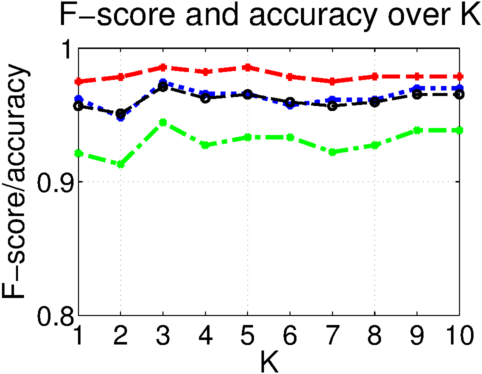
\includegraphics[width=0.3\textwidth]{tex/appendices/test/mfcc2010FP.png}
	\centering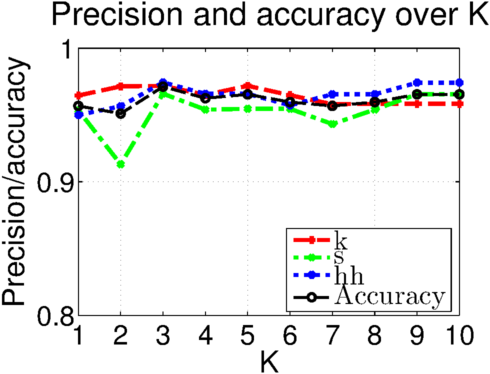
\includegraphics[width=0.3\textwidth]{tex/appendices/test/mfcc2010_P.png}
	\centering\includegraphics[width=0.3\textwidth]{tex/appendices/test/mfcc2010_R.png}
	
	\caption{Plots over K for MFCC with 20ms windows and 10ms window skips}
\end{figure}
\begin{figure}


	\centering\includegraphics[width=0.3\textwidth]{tex/appendices/test/mfcc105FP.png}
	\centering\includegraphics[width=0.3\textwidth]{tex/appendices/test/mfcc105_P.png}
	\centering\includegraphics[width=0.3\textwidth]{tex/appendices/test/mfcc105_R.png}
	
	\caption{Plots over K for MFCC with 10ms windows and 5ms window skips}
\end{figure}
\begin{figure}


	\centering\includegraphics[width=0.3\textwidth]{tex/appendices/test/mfcc52FP.png}
	\centering\includegraphics[width=0.3\textwidth]{tex/appendices/test/mfcc52_P.png}
	\centering\includegraphics[width=0.3\textwidth]{tex/appendices/test/mfcc52_R.png}
	
	\caption{Plots over K for MFCC with 5ms windows and 2ms window skips}
\end{figure}\clearpage


\begin{table}
\begin{subtable}[tbp]{0.45\textwidth}
\centering
\begin{tabular}{|c|c|c|c"c|}
\cline{2-5}
 \multicolumn{1}{c|}{} & \textbf{k}  & \textbf{s}  & \textbf{hh}  & Prec.\\ \hline
 \textbf{k} & \textcolor{red}{0.986} & 0.054 & 0.000 & 0.965\\ \hline
 \textbf{s} & 0.007 & \textcolor{red}{0.891} & 0.026 & 0.953\\ \hline
 \textbf{hh} & 0.007 & 0.054 & \textcolor{red}{0.974} & 0.950\\ \Xhline{2\arrayrulewidth}
 F & 0.975 & 0.921 & 0.962 & \textcolor{blue}{0.957}\\ \hline
\end{tabular}
\caption{$K=1$}
\end{subtable}
\hfill
\begin{subtable}[tbp]{0.45\textwidth}
\centering
\begin{tabular}{|c|c|c|c"c|}
\cline{2-5}
 \multicolumn{1}{c|}{} & \textbf{k}  & \textbf{s}  & \textbf{hh}  & Prec.\\ \hline
 \textbf{k} & \textcolor{red}{0.986} & 0.043 & 0.000 & 0.971\\ \hline
 \textbf{s} & 0.007 & \textcolor{red}{0.913} & 0.060 & 0.913\\ \hline
 \textbf{hh} & 0.007 & 0.043 & \textcolor{red}{0.940} & 0.957\\ \Xhline{2\arrayrulewidth}
 F & 0.978 & 0.913 & 0.948 & \textcolor{blue}{0.951}\\ \hline
\end{tabular}
\caption{$K=2$}
\label{app:Mfcc:2:worst}
\end{subtable}
\hfill
\begin{subtable}[tbp]{0.45\textwidth}
\centering
\begin{tabular}{|c|c|c|c"c|}
\cline{2-5}
 \multicolumn{1}{c|}{} & \textbf{k}  & \textbf{s}  & \textbf{hh}  & Prec.\\ \hline
 \textbf{k} & \textcolor{red}{1.000} & 0.043 & 0.000 & 0.972\\ \hline
 \textbf{s} & 0.000 & \textcolor{red}{0.924} & 0.026 & 0.966\\ \hline
 \textbf{hh} & 0.000 & 0.033 & \textcolor{red}{0.974} & 0.974\\ \Xhline{2\arrayrulewidth}
 F & 0.986 & 0.944 & 0.974 & \textcolor{blue}{0.971}\\ \hline
\end{tabular}
\caption{$K=3$}
\end{subtable}
\hfill
\begin{subtable}[tbp]{0.45\textwidth}
\centering
\begin{tabular}{|c|c|c|c"c|}
\cline{2-5}
 \multicolumn{1}{c|}{} & \textbf{k}  & \textbf{s}  & \textbf{hh}  & Prec.\\ \hline
 \textbf{k} & \textcolor{red}{1.000} & 0.054 & 0.000 & 0.965\\ \hline
 \textbf{s} & 0.000 & \textcolor{red}{0.902} & 0.034 & 0.954\\ \hline
 \textbf{hh} & 0.000 & 0.043 & \textcolor{red}{0.966} & 0.966\\ \Xhline{2\arrayrulewidth}
 F & 0.982 & 0.927 & 0.966 & \textcolor{blue}{0.963}\\ \hline
\end{tabular}
\caption{$K=4$}
\end{subtable}
\hfill
\begin{subtable}[tbp]{0.45\textwidth}
\centering
\begin{tabular}{|c|c|c|c"c|}
\cline{2-5}
 \multicolumn{1}{c|}{} & \textbf{k}  & \textbf{s}  & \textbf{hh}  & Prec.\\ \hline
 \textbf{k} & \textcolor{red}{1.000} & 0.043 & 0.000 & 0.972\\ \hline
 \textbf{s} & 0.000 & \textcolor{red}{0.913} & 0.034 & 0.955\\ \hline
 \textbf{hh} & 0.000 & 0.043 & \textcolor{red}{0.966} & 0.966\\ \Xhline{2\arrayrulewidth}
 F & 0.986 & 0.933 & 0.966 & \textcolor{blue}{0.965}\\ \hline
\end{tabular}
\caption{$K=5$}
\end{subtable}
\hfill
\begin{subtable}[tbp]{0.45\textwidth}
\centering
\begin{tabular}{|c|c|c|c"c|}
\cline{2-5}
 \multicolumn{1}{c|}{} & \textbf{k}  & \textbf{s}  & \textbf{hh}  & Prec.\\ \hline
 \textbf{k} & \textcolor{red}{0.993} & 0.043 & 0.009 & 0.965\\ \hline
 \textbf{s} & 0.000 & \textcolor{red}{0.913} & 0.034 & 0.955\\ \hline
 \textbf{hh} & 0.000 & 0.043 & \textcolor{red}{0.957} & 0.957\\ \Xhline{2\arrayrulewidth}
 F & 0.979 & 0.933 & 0.957 & \textcolor{blue}{0.960}\\ \hline
\end{tabular}
\caption{$K=6$}
\end{subtable}
\hfill
\begin{subtable}[tbp]{0.45\textwidth}
\centering
\begin{tabular}{|c|c|c|c"c|}
\cline{2-5}
 \multicolumn{1}{c|}{} & \textbf{k}  & \textbf{s}  & \textbf{hh}  & Prec.\\ \hline
 \textbf{k} & \textcolor{red}{0.993} & 0.054 & 0.009 & 0.958\\ \hline
 \textbf{s} & 0.007 & \textcolor{red}{0.902} & 0.034 & 0.943\\ \hline
 \textbf{hh} & 0.007 & 0.043 & \textcolor{red}{0.957} & 0.966\\ \Xhline{2\arrayrulewidth}
 F & 0.975 & 0.922 & 0.961 & \textcolor{blue}{0.957}\\ \hline
\end{tabular}
\caption{$K=7$}
\end{subtable}
\hfill
\begin{subtable}[tbp]{0.45\textwidth}
\centering
\begin{tabular}{|c|c|c|c"c|}
\cline{2-5}
 \multicolumn{1}{c|}{} & \textbf{k}  & \textbf{s}  & \textbf{hh}  & Prec.\\ \hline
 \textbf{k} & \textcolor{red}{1.000} & 0.054 & 0.009 & 0.958\\ \hline
 \textbf{s} & 0.000 & \textcolor{red}{0.902} & 0.034 & 0.954\\ \hline
 \textbf{hh} & 0.000 & 0.043 & \textcolor{red}{0.957} & 0.966\\ \Xhline{2\arrayrulewidth}
 F & 0.979 & 0.927 & 0.961 & \textcolor{blue}{0.960}\\ \hline
\end{tabular}
\caption{$K=8$}
\end{subtable}
\hfill
\begin{subtable}[tbp]{0.45\textwidth}
\centering
\begin{tabular}{|c|c|c|c"c|}
\cline{2-5}
 \multicolumn{1}{c|}{} & \textbf{k}  & \textbf{s}  & \textbf{hh}  & Prec.\\ \hline
 \textbf{k} & \textcolor{red}{1.000} & 0.054 & 0.009 & 0.958\\ \hline
 \textbf{s} & 0.000 & \textcolor{red}{0.913} & 0.026 & 0.966\\ \hline
 \textbf{hh} & 0.000 & 0.033 & \textcolor{red}{0.966} & 0.974\\ \Xhline{2\arrayrulewidth}
 F & 0.979 & 0.939 & 0.970 & \textcolor{blue}{0.965}\\ \hline
\end{tabular}
\caption{$K=9$}
\end{subtable}
\hfill
\begin{subtable}[tbp]{0.45\textwidth}
\centering
\begin{tabular}{|c|c|c|c"c|}
\cline{2-5}
 \multicolumn{1}{c|}{} & \textbf{k}  & \textbf{s}  & \textbf{hh}  & Prec.\\ \hline
 \textbf{k} & \textcolor{red}{1.000} & 0.054 & 0.009 & 0.958\\ \hline
 \textbf{s} & 0.000 & \textcolor{red}{0.913} & 0.026 & 0.966\\ \hline
 \textbf{hh} & 0.000 & 0.033 & \textcolor{red}{0.966} & 0.974\\ \Xhline{2\arrayrulewidth}
 F & 0.979 & 0.939 & 0.970 & \textcolor{blue}{0.965}\\ \hline
\end{tabular}
\caption{$K=10$}
\end{subtable}
\hfill

\caption{tcmfcc2010}
\label{tlmfcc2010}


\end{table}\clearpage


\begin{table}

\begin{subtable}[tbp]{0.45\textwidth}
\centering
 
\scalebox{0.8}{\begin{tabular}{|c|c|c|c|}\hline
 $K_1$ & $K_2$ & $X^2$ & p\\ \hline
 1 & 2 & 54.000 & 0.02745\\ \hline 
 1 & 3 & 38.250 & 0.14355\\ \hline 
 1 & 4 & 38.250 & 0.14355\\ \hline 
 1 & 5 & 36.000 & 0.05490\\ \hline 
 1 & 6 & 38.250 & 0.14355\\ \hline 
 1 & 7 & 40.500 & 0.27855\\ \hline 
 1 & 8 & 47.250 & 0.09945\\ \hline 
 1 & 9 & 47.250 & 0.09945\\ \hline 
 1 & 10 & 47.250 & 0.09945\\ \hline 
 2 & 3 & 38.250 & 0.14355\\ \hline 
 2 & 4 & 38.250 & 0.14355\\ \hline 
 2 & 5 & 36.000 & 0.05490\\ \hline 
 2 & 6 & 38.250 & 0.14355\\ \hline 
 2 & 7 & 40.500 & 0.27855\\ \hline 
 2 & 8 & 47.250 & 0.09945\\ \hline 
 2 & 9 & 47.250 & 0.09945\\ \hline 
 2 & 10 & 47.250 & 0.09945\\ \hline 
 3 & 4 & 45.000 & 0.00855\\ \hline 
 3 & 5 & 36.000 & 0.01530\\ \hline 
 3 & 6 & 36.000 & 0.07155\\ \hline 
 3 & 7 & 45.000 & 0.03870\\ \hline 
 3 & 8 & 45.000 & 0.03870\\ \hline 
 3 & 9 & 45.000 & 0.03870\\ \hline 
 3 & 10 & 45.000 & 0.03870\\ \hline 
 4 & 5 & 36.000 & 0.01530\\ \hline 
 4 & 6 & 36.000 & 0.07155\\ \hline 
 4 & 7 & 45.000 & 0.03870\\ \hline 
 4 & 8 & 45.000 & 0.03870\\ \hline 
 4 & 9 & 45.000 & 0.03870\\ \hline 
 4 & 10 & 45.000 & 0.03870\\ \hline 
 5 & 6 & 36.000 & 0.01530\\ \hline 
 5 & 7 & 36.000 & 0.05490\\ \hline 
 5 & 8 & 36.000 & 0.05490\\ \hline 
 5 & 9 & 36.000 & 0.05490\\ \hline 
 5 & 10 & 36.000 & 0.05490\\ \hline 
 6 & 7 & 38.250 & 0.14355\\ \hline 
 6 & 8 & 38.250 & 0.14355\\ \hline 
 6 & 9 & 38.250 & 0.14355\\ \hline 
 6 & 10 & 38.250 & 0.14355\\ \hline 
 7 & 8 & 47.250 & 0.09945\\ \hline 
 7 & 9 & 47.250 & 0.09945\\ \hline 
 7 & 10 & 47.250 & 0.09945\\ \hline 
 8 & 9 & 54.000 & 0.02745\\ \hline 
 8 & 10 & 54.000 & 0.02745\\ \hline 
 9 & 10 & 54.000 & 0.02745\\ \hline 

\end{tabular}
} 
\caption{xcmfcc2010}
\label{xlmfcc2010}
\end{subtable}

\begin{subtable}[tbp]{0.45\textwidth}
\centering
\begin{tabular}{|c|c|c|}
\hline
Class & Amount & Percent\\ \hline
k & 322 & 39.80\\ \hline
s & 214 & 26.45\\ \hline
hh & 273 & 33.75\\ \hline
\end{tabular}
\caption{Training dataset}
\end{subtable}
\hfill
\begin{subtable}[tbp]{0.45\textwidth}
\centering
\begin{tabular}{|c|c|c|}
\hline
Class & Amount & Percent\\ \hline
k & 138 & 39.77\\ \hline
s & 92 & 26.51\\ \hline
hh & 117 & 33.72\\ \hline
\end{tabular}
\caption{Testing dataset}
\end{subtable}
\hfill

\caption{dcmfcc2010}

\label{dlmfcc2010}

\end{table}\clearpage


\begin{table}
\begin{subtable}[tbp]{0.45\textwidth}
\centering
\begin{tabular}{|c|c|c|c"c|}
\cline{2-5}
 \multicolumn{1}{c|}{} & \textbf{k}  & \textbf{s}  & \textbf{hh}  & Prec.\\ \hline
 \textbf{k} & \textcolor{red}{0.978} & 0.031 & 0.017 & 0.965\\ \hline
 \textbf{s} & 0.022 & \textcolor{red}{0.929} & 0.034 & 0.929\\ \hline
 \textbf{hh} & 0.022 & 0.041 & \textcolor{red}{0.949} & 0.966\\ \Xhline{2\arrayrulewidth}
 F & 0.971 & 0.929 & 0.957 & \textcolor{blue}{0.955}\\ \hline
\end{tabular}
\caption{$K=1$}
\end{subtable}
\hfill
\begin{subtable}[tbp]{0.45\textwidth}
\centering
\begin{tabular}{|c|c|c|c"c|}
\cline{2-5}
 \multicolumn{1}{c|}{} & \textbf{k}  & \textbf{s}  & \textbf{hh}  & Prec.\\ \hline
 \textbf{k} & \textcolor{red}{0.978} & 0.010 & 0.017 & 0.978\\ \hline
 \textbf{s} & 0.022 & \textcolor{red}{0.959} & 0.025 & 0.940\\ \hline
 \textbf{hh} & 0.022 & 0.031 & \textcolor{red}{0.958} & 0.974\\ \Xhline{2\arrayrulewidth}
 F & 0.978 & 0.949 & 0.966 & \textcolor{blue}{0.966}\\ \hline
\end{tabular}
\caption{$K=2$}
\end{subtable}
\hfill
\begin{subtable}[tbp]{0.45\textwidth}
\centering
\begin{tabular}{|c|c|c|c"c|}
\cline{2-5}
 \multicolumn{1}{c|}{} & \textbf{k}  & \textbf{s}  & \textbf{hh}  & Prec.\\ \hline
 \textbf{k} & \textcolor{red}{0.993} & 0.020 & 0.017 & 0.972\\ \hline
 \textbf{s} & 0.007 & \textcolor{red}{0.939} & 0.025 & 0.958\\ \hline
 \textbf{hh} & 0.007 & 0.041 & \textcolor{red}{0.958} & 0.966\\ \Xhline{2\arrayrulewidth}
 F & 0.982 & 0.948 & 0.962 & \textcolor{blue}{0.966}\\ \hline
\end{tabular}
\caption{$K=3$}
\end{subtable}
\hfill
\begin{subtable}[tbp]{0.45\textwidth}
\centering
\begin{tabular}{|c|c|c|c"c|}
\cline{2-5}
 \multicolumn{1}{c|}{} & \textbf{k}  & \textbf{s}  & \textbf{hh}  & Prec.\\ \hline
 \textbf{k} & \textcolor{red}{0.986} & 0.010 & 0.017 & 0.979\\ \hline
 \textbf{s} & 0.014 & \textcolor{red}{0.959} & 0.025 & 0.949\\ \hline
 \textbf{hh} & 0.014 & 0.031 & \textcolor{red}{0.958} & 0.974\\ \Xhline{2\arrayrulewidth}
 F & 0.982 & 0.954 & 0.966 & \textcolor{blue}{0.969}\\ \hline
\end{tabular}
\caption{$K=4$}
\end{subtable}
\hfill
\begin{subtable}[tbp]{0.45\textwidth}
\centering
\begin{tabular}{|c|c|c|c"c|}
\cline{2-5}
 \multicolumn{1}{c|}{} & \textbf{k}  & \textbf{s}  & \textbf{hh}  & Prec.\\ \hline
 \textbf{k} & \textcolor{red}{0.993} & 0.010 & 0.017 & 0.979\\ \hline
 \textbf{s} & 0.007 & \textcolor{red}{0.949} & 0.025 & 0.959\\ \hline
 \textbf{hh} & 0.007 & 0.041 & \textcolor{red}{0.958} & 0.966\\ \Xhline{2\arrayrulewidth}
 F & 0.986 & 0.954 & 0.962 & \textcolor{blue}{0.969}\\ \hline
\end{tabular}
\caption{$K=5$}
\end{subtable}
\hfill
\begin{subtable}[tbp]{0.45\textwidth}
\centering
\begin{tabular}{|c|c|c|c"c|}
\cline{2-5}
 \multicolumn{1}{c|}{} & \textbf{k}  & \textbf{s}  & \textbf{hh}  & Prec.\\ \hline
 \textbf{k} & \textcolor{red}{0.993} & 0.010 & 0.017 & 0.979\\ \hline
 \textbf{s} & 0.007 & \textcolor{red}{0.949} & 0.025 & 0.959\\ \hline
 \textbf{hh} & 0.007 & 0.041 & \textcolor{red}{0.958} & 0.966\\ \Xhline{2\arrayrulewidth}
 F & 0.986 & 0.954 & 0.962 & \textcolor{blue}{0.969}\\ \hline
\end{tabular}
\caption{$K=6$}
\end{subtable}
\hfill
\begin{subtable}[tbp]{0.45\textwidth}
\centering
\begin{tabular}{|c|c|c|c"c|}
\cline{2-5}
 \multicolumn{1}{c|}{} & \textbf{k}  & \textbf{s}  & \textbf{hh}  & Prec.\\ \hline
 \textbf{k} & \textcolor{red}{0.993} & 0.010 & 0.017 & 0.979\\ \hline
 \textbf{s} & 0.007 & \textcolor{red}{0.959} & 0.025 & 0.959\\ \hline
 \textbf{hh} & 0.007 & 0.031 & \textcolor{red}{0.958} & 0.974\\ \Xhline{2\arrayrulewidth}
 F & 0.986 & 0.959 & 0.966 & \textcolor{blue}{0.972}\\ \hline
\end{tabular}
\caption{$K=7$}
\end{subtable}
\hfill
\begin{subtable}[tbp]{0.45\textwidth}
\centering
\begin{tabular}{|c|c|c|c"c|}
\cline{2-5}
 \multicolumn{1}{c|}{} & \textbf{k}  & \textbf{s}  & \textbf{hh}  & Prec.\\ \hline
 \textbf{k} & \textcolor{red}{0.986} & 0.010 & 0.017 & 0.979\\ \hline
 \textbf{s} & 0.014 & \textcolor{red}{0.949} & 0.025 & 0.949\\ \hline
 \textbf{hh} & 0.014 & 0.041 & \textcolor{red}{0.958} & 0.966\\ \Xhline{2\arrayrulewidth}
 F & 0.982 & 0.949 & 0.962 & \textcolor{blue}{0.966}\\ \hline
\end{tabular}
\caption{$K=8$}
\end{subtable}
\hfill
\begin{subtable}[tbp]{0.45\textwidth}
\centering
\begin{tabular}{|c|c|c|c"c|}
\cline{2-5}
 \multicolumn{1}{c|}{} & \textbf{k}  & \textbf{s}  & \textbf{hh}  & Prec.\\ \hline
 \textbf{k} & \textcolor{red}{0.993} & 0.010 & 0.017 & 0.979\\ \hline
 \textbf{s} & 0.007 & \textcolor{red}{0.949} & 0.017 & 0.969\\ \hline
 \textbf{hh} & 0.007 & 0.041 & \textcolor{red}{0.966} & 0.966\\ \Xhline{2\arrayrulewidth}
 F & 0.986 & 0.959 & 0.966 & \textcolor{blue}{0.972}\\ \hline
\end{tabular}
\caption{$K=9$}
\end{subtable}
\hfill
\begin{subtable}[tbp]{0.45\textwidth}
\centering
\begin{tabular}{|c|c|c|c"c|}
\cline{2-5}
 \multicolumn{1}{c|}{} & \textbf{k}  & \textbf{s}  & \textbf{hh}  & Prec.\\ \hline
 \textbf{k} & \textcolor{red}{0.993} & 0.010 & 0.017 & 0.979\\ \hline
 \textbf{s} & 0.007 & \textcolor{red}{0.959} & 0.017 & 0.969\\ \hline
 \textbf{hh} & 0.007 & 0.031 & \textcolor{red}{0.966} & 0.974\\ \Xhline{2\arrayrulewidth}
 F & 0.986 & 0.964 & 0.970 & \textcolor{blue}{0.975}\\ \hline
\end{tabular}
\caption{$K=10$}
\end{subtable}
\hfill


\caption{tcmfcc105}
\label{tlmfcc105}

\end{table}\clearpage


\begin{table}

\begin{subtable}[tbp]{0.45\textwidth}
\centering
 
\scalebox{0.8}{\begin{tabular}{|c|c|c|c|}\hline
 $K_1$ & $K_2$ & $X^2$ & p\\ \hline
 1 & 2 & 48.000 & 0.08730\\ \hline 
 1 & 3 & 47.250 & 0.26685\\ \hline   
 1 & 4 & 47.250 & 0.09945\\ \hline 
 1 & 5 & 54.000 & 0.10125\\ \hline 
 1 & 6 & 54.000 & 0.10125\\ \hline 
 1 & 7 & 54.000 & 0.02745\\ \hline 
 1 & 8 & 47.250 & 0.26685\\ \hline 
 1 & 9 & 47.250 & 0.09945\\ \hline 
 1 & 10 & 47.250 & 0.09945\\ \hline 
 2 & 3 & 45.000 & 0.3474\\ \hline 
 2 & 4 & 48.000 & 0.08730\\ \hline 
 2 & 5 & 48.000 & 0.26685\\ \hline 
 2 & 6 & 48.000 & 0.26685\\ \hline 
 2 & 7 & 48.000 & 0.08730\\ \hline 
 2 & 8 & 48.000 & 0.26685\\ \hline 
 2 & 9 & 42.000 & 0.22680\\ \hline 
 2 & 10 & 42.000 & 0.22680\\ \hline 
 3 & 4 & 47.250 & 0.26685\\ \hline 
 3 & 5 & 56.250 & 0.22185\\ \hline 
 3 & 6 & 56.250 & 0.22185\\ \hline 
 3 & 7 & 47.250 & 0.26685\\ \hline 
 3 & 8 & 56.250 & 0.22185\\ \hline 
 3 & 9 & 49.500 & 0.19890\\ \hline 
 3 & 10 & 49.500 & 0.19890\\ \hline 
 4 & 5 & 47.250 & 0.26685\\ \hline 
 4 & 6 & 47.250 & 0.26685\\ \hline 
 4 & 7 & 47.250 & 0.09945\\ \hline 
 4 & 8 & 54.000 & 0.10125\\ \hline 
 4 & 9 & 42.750 & 0.20385\\ \hline 
 4 & 10 & 42.750 & 0.20385\\ \hline 
 5 & 6 & 63.000 & 0.08640\\ \hline 
 5 & 7 & 54.000 & 0.10125\\ \hline 
 5 & 8 & 56.250 & 0.22185\\ \hline 
 5 & 9 & 54.000 & 0.10125\\ \hline 
 5 & 10 & 54.000 & 0.10125\\ \hline 
 6 & 7 & 54.000 & 0.10125\\ \hline 
 6 & 8 & 56.250 & 0.22185\\ \hline 
 6 & 9 & 54.000 & 0.10125\\ \hline 
 6 & 10 & 54.000 & 0.10125\\ \hline 
 7 & 8 & 47.250 & 0.26685\\ \hline 
 7 & 9 & 47.250 & 0.09945\\ \hline 
 7 & 10 & 47.250 & 0.09945\\ \hline 
 8 & 9 & 49.500 & 0.19890\\ \hline 
 8 & 10 & 49.500 & 0.19890\\ \hline 
 9 & 10 & 54.000 & 0.02745\\ \hline 

\end{tabular}
}\caption{xcmfcc105} \label{xlmfcc105}

\end{subtable}

\begin{subtable}[tbp]{0.45\textwidth}
\centering
\begin{tabular}{|c|c|c|}
\hline
Class & Amount & Percent\\ \hline
k & 326 & 39.23\\ \hline
s & 229 & 27.56\\ \hline
hh & 276 & 33.21\\ \hline
\end{tabular}
\caption{Training dataset}
\end{subtable}
\hfill
\begin{subtable}[tbp]{0.45\textwidth}
\centering
\begin{tabular}{|c|c|c|}
\hline
Class & Amount & Percent\\ \hline
k & 139 & 39.15\\ \hline
s & 98 & 27.61\\ \hline
hh & 118 & 33.24\\ \hline
\end{tabular}
\caption{Testing dataset}
\end{subtable}
\hfill

\caption{dcmfcc105}
\label{dlmfcc105}


\end{table}\clearpage


\begin{table}
\begin{subtable}[tbp]{0.45\textwidth}
\centering
\begin{tabular}{|c|c|c|c"c|}
\cline{2-5}
 \multicolumn{1}{c|}{} & \textbf{k}  & \textbf{s}  & \textbf{hh}  & Prec.\\ \hline
 \textbf{k} & \textcolor{red}{0.986} & 0.020 & 0.008 & 0.979\\ \hline
 \textbf{s} & 0.007 & \textcolor{red}{0.949} & 0.025 & 0.959\\ \hline
 \textbf{hh} & 0.007 & 0.030 & \textcolor{red}{0.966} & 0.966\\ \Xhline{2\arrayrulewidth}
 F & 0.982 & 0.954 & 0.966 & \textcolor{blue}{0.969}\\ \hline
\end{tabular}
\caption{$K=1$}
\end{subtable}
\hfill
\begin{subtable}[tbp]{0.45\textwidth}
\centering
\begin{tabular}{|c|c|c|c"c|}
\cline{2-5}
 \multicolumn{1}{c|}{} & \textbf{k}  & \textbf{s}  & \textbf{hh}  & Prec.\\ \hline
 \textbf{k} & \textcolor{red}{0.986} & 0.020 & 0.008 & 0.979\\ \hline
 \textbf{s} & 0.014 & \textcolor{red}{0.949} & 0.008 & 0.969\\ \hline
 \textbf{hh} & 0.014 & 0.030 & \textcolor{red}{0.983} & 0.975\\ \Xhline{2\arrayrulewidth}
 F & 0.982 & 0.959 & 0.979 & \textcolor{blue}{0.975}\\ \hline
\end{tabular}
\caption{$K=2$}
\end{subtable}
\hfill
\begin{subtable}[tbp]{0.45\textwidth}
\centering
\begin{tabular}{|c|c|c|c"c|}
\cline{2-5}
 \multicolumn{1}{c|}{} & \textbf{k}  & \textbf{s}  & \textbf{hh}  & Prec.\\ \hline
 \textbf{k} & \textcolor{red}{1.000} & 0.010 & 0.008 & 0.986\\ \hline
 \textbf{s} & 0.000 & \textcolor{red}{0.970} & 0.008 & 0.990\\ \hline
 \textbf{hh} & 0.000 & 0.020 & \textcolor{red}{0.983} & 0.983\\ \Xhline{2\arrayrulewidth}
 F & 0.993 & 0.980 & 0.983 & \textcolor{blue}{0.986}\\ \hline
\end{tabular}
\caption{$K=3$}
\end{subtable}
\hfill
\begin{subtable}[tbp]{0.45\textwidth}
\centering
\begin{tabular}{|c|c|c|c"c|}
\cline{2-5}
 \multicolumn{1}{c|}{} & \textbf{k}  & \textbf{s}  & \textbf{hh}  & Prec.\\ \hline
 \textbf{k} & \textcolor{red}{1.000} & 0.010 & 0.008 & 0.986\\ \hline
 \textbf{s} & 0.000 & \textcolor{red}{0.960} & 0.008 & 0.990\\ \hline
 \textbf{hh} & 0.000 & 0.030 & \textcolor{red}{0.983} & 0.975\\ \Xhline{2\arrayrulewidth}
 F & 0.993 & 0.974 & 0.979 & \textcolor{blue}{0.983}\\ \hline
\end{tabular}
\caption{$K=4$}
\end{subtable}
\hfill
\begin{subtable}[tbp]{0.45\textwidth}
\centering
\begin{tabular}{|c|c|c|c"c|}
\cline{2-5}
 \multicolumn{1}{c|}{} & \textbf{k}  & \textbf{s}  & \textbf{hh}  & Prec.\\ \hline
 \textbf{k} & \textcolor{red}{1.000} & 0.010 & 0.008 & 0.986\\ \hline
 \textbf{s} & 0.000 & \textcolor{red}{0.970} & 0.008 & 0.990\\ \hline
 \textbf{hh} & 0.000 & 0.020 & \textcolor{red}{0.983} & 0.983\\ \Xhline{2\arrayrulewidth}
 F & 0.993 & 0.980 & 0.983 & \textcolor{blue}{0.986}\\ \hline
\end{tabular}
\caption{$K=5$}
\end{subtable}
\hfill
\begin{subtable}[tbp]{0.45\textwidth}
\centering
\begin{tabular}{|c|c|c|c"c|}
\cline{2-5}
 \multicolumn{1}{c|}{} & \textbf{k}  & \textbf{s}  & \textbf{hh}  & Prec.\\ \hline
 \textbf{k} & \textcolor{red}{0.993} & 0.010 & 0.008 & 0.986\\ \hline
 \textbf{s} & 0.007 & \textcolor{red}{0.980} & 0.008 & 0.980\\ \hline
 \textbf{hh} & 0.007 & 0.010 & \textcolor{red}{0.983} & 0.991\\ \Xhline{2\arrayrulewidth}
 F & 0.989 & 0.980 & 0.987 & \textcolor{blue}{0.986}\\ \hline
\end{tabular}
\caption{$K=6$}
\end{subtable}
\hfill
\begin{subtable}[tbp]{0.45\textwidth}
\centering
\begin{tabular}{|c|c|c|c"c|}
\cline{2-5}
 \multicolumn{1}{c|}{} & \textbf{k}  & \textbf{s}  & \textbf{hh}  & Prec.\\ \hline
 \textbf{k} & \textcolor{red}{1.000} & 0.010 & 0.008 & 0.986\\ \hline
 \textbf{s} & 0.000 & \textcolor{red}{0.980} & 0.008 & 0.990\\ \hline
 \textbf{hh} & 0.000 & 0.010 & \textcolor{red}{0.983} & 0.991\\ \Xhline{2\arrayrulewidth}
 F & 0.993 & 0.985 & 0.987 & \textcolor{blue}{0.989}\\ \hline
\end{tabular}
\caption{$K=7$}
\label{app:MFCC:7:best}
\end{subtable}
\hfill
\begin{subtable}[tbp]{0.45\textwidth}
\centering
\begin{tabular}{|c|c|c|c"c|}
\cline{2-5}
 \multicolumn{1}{c|}{} & \textbf{k}  & \textbf{s}  & \textbf{hh}  & Prec.\\ \hline
 \textbf{k} & \textcolor{red}{1.000} & 0.010 & 0.008 & 0.986\\ \hline
 \textbf{s} & 0.000 & \textcolor{red}{0.980} & 0.008 & 0.990\\ \hline
 \textbf{hh} & 0.000 & 0.010 & \textcolor{red}{0.983} & 0.991\\ \Xhline{2\arrayrulewidth}
 F & 0.993 & 0.985 & 0.987 & \textcolor{blue}{0.989}\\ \hline
\end{tabular}
\caption{$K=8$}
\label{app:MFCC:8:best}
\end{subtable}
\hfill
\begin{subtable}[tbp]{0.45\textwidth}
\centering
\begin{tabular}{|c|c|c|c"c|}
\cline{2-5}
 \multicolumn{1}{c|}{} & \textbf{k}  & \textbf{s}  & \textbf{hh}  & Prec.\\ \hline
 \textbf{k} & \textcolor{red}{0.993} & 0.010 & 0.008 & 0.986\\ \hline
 \textbf{s} & 0.007 & \textcolor{red}{0.980} & 0.008 & 0.980\\ \hline
 \textbf{hh} & 0.007 & 0.010 & \textcolor{red}{0.983} & 0.991\\ \Xhline{2\arrayrulewidth}
 F & 0.989 & 0.980 & 0.987 & \textcolor{blue}{0.986}\\ \hline
\end{tabular}
\caption{$K=9$}
\end{subtable}
\hfill
\begin{subtable}[tbp]{0.45\textwidth}
\centering
\begin{tabular}{|c|c|c|c"c|}
\cline{2-5}
 \multicolumn{1}{c|}{} & \textbf{k}  & \textbf{s}  & \textbf{hh}  & Prec.\\ \hline
 \textbf{k} & \textcolor{red}{0.993} & 0.010 & 0.008 & 0.986\\ \hline
 \textbf{s} & 0.007 & \textcolor{red}{0.970} & 0.000 & 0.990\\ \hline
 \textbf{hh} & 0.007 & 0.020 & \textcolor{red}{0.992} & 0.983\\ \Xhline{2\arrayrulewidth}
 F & 0.989 & 0.980 & 0.987 & \textcolor{blue}{0.986}\\ \hline
\end{tabular}
\caption{$K=10$}
\end{subtable}
\hfill

\caption{tcmfcc52}
\label{tlmfcc52}


\end{table}\clearpage


\begin{table}

\begin{subtable}[tbp]{0.45\textwidth}
\centering
 
\scalebox{0.8}{\begin{tabular}{|c|c|c|c|}\hline
 $K_1$ & $K_2$ & $X^2$ & p\\ \hline
 1 & 2 & 35.250 & 0.23355\\ \hline 
 1 & 3 & 34.000 & 0.10800\\ \hline 
 1 & 4 & 34.000 & 0.10800\\ \hline 
 1 & 5 & 34.000 & 0.10800\\ \hline 
 1 & 6 & 28.800 & 0.09180\\ \hline 
 1 & 7 & 31.500 & 0.04905\\ \hline 
 1 & 8 & 31.500 & 0.04905\\ \hline 
 1 & 9 & 28.800 & 0.09180\\ \hline 
 1 & 10 & 33.250 & 0.12510\\ \hline 
 2 & 3 & 41.250 & 0.0018\\ \hline 
 2 & 4 & 41.250 & 0.0828\\ \hline 
 2 & 5 & 41.250 & 0.0828\\ \hline 
 2 & 6 & 36.000 & 0.05490\\ \hline 
 2 & 7 & 32.625 & 0.11205\\ \hline 
 2 & 8 & 32.625 & 0.11205\\ \hline 
 2 & 9 & 36.000 & 0.05490\\ \hline 
 2 & 10 & 41.250 & 0.0828\\ \hline 
 3 & 4 & 45.000 & 0.00855\\ \hline 
 3 & 5 & 45.000 & 0.00855\\ \hline 
 3 & 6 & 30.600 & 0.0603\\ \hline 
 3 & 7 & 36.000 & 0.01530\\ \hline 
 3 & 8 & 36.000 & 0.01530\\ \hline 
 3 & 9 & 30.600 & 0.0603\\ \hline 
 3 & 10 & 36.250 & 0.06795\\ \hline 
 4 & 5 & 45.000 & 0.00855\\ \hline 
 4 & 6 & 30.600 & 0.0603\\ \hline 
 4 & 7 & 36.000 & 0.01530\\ \hline 
 4 & 8 & 36.000 & 0.01530\\ \hline 
 4 & 9 & 30.600 & 0.0603\\ \hline 
 4 & 10 & 36.250 & 0.06795\\ \hline 
 5 & 6 & 30.600 & 0.0603\\ \hline 
 5 & 7 & 36.000 & 0.01530\\ \hline 
 5 & 8 & 36.000 & 0.01530\\ \hline 
 5 & 9 & 30.600 & 0.0603\\ \hline 
 5 & 10 & 36.250 & 0.06795\\ \hline 
 6 & 7 & 30.600 & 0.01530\\ \hline 
 6 & 8 & 30.600 & 0.01530\\ \hline 
 6 & 9 & 36.000 & 0.00270\\ \hline 
 6 & 10 & 30.600 & 0.0603\\ \hline 
 7 & 8 & 36.000 & 0.00270\\ \hline 
 7 & 9 & 30.600 & 0.01530\\ \hline 
 7 & 10 & 28.125 & 0.10665\\ \hline 
 8 & 9 & 30.600 & 0.01530\\ \hline 
 8 & 10 & 28.125 & 0.10665\\ \hline 
 9 & 10 & 30.600 & 0.0603\\ \hline 

\end{tabular}
} \caption{xcmfcc52}\label{xlmfcc52}

\end{subtable}

\begin{subtable}[tbp]{0.45\textwidth}
\centering
\begin{tabular}{|c|c|c|}
\hline
Class & Amount & Percent\\ \hline
k & 326 & 39.14\\ \hline
s & 231 & 27.73\\ \hline
hh & 276 & 33.13\\ \hline
\end{tabular}
\caption{Training dataset}
\end{subtable}
\hfill
\begin{subtable}[tbp]{0.45\textwidth}
\centering
\begin{tabular}{|c|c|c|}
\hline
Class & Amount & Percent\\ \hline
k & 139 & 39.04\\ \hline
s & 99 & 27.81\\ \hline
hh & 118 & 33.15\\ \hline
\end{tabular}
\caption{Testing dataset}
\end{subtable}
\hfill


\caption{dcmfcc52}

\label{dlmfcc52}
\end{table}\clearpage


\subsection{Spectral Centroid}
	\label{app:res:sc}
	\begin{figure}


	\centering\includegraphics[width=0.3\textwidth]{tex/appendices/test/scentroid2010FP.png}
	\centering\includegraphics[width=0.3\textwidth]{tex/appendices/test/scentroid2010_P.png}
	\centering\includegraphics[width=0.3\textwidth]{tex/appendices/test/scentroid2010_R.png}
	
	\caption{Plots over K for Spectral Centroid with 20ms windows and 10ms window skips}
\end{figure}
\begin{figure}


	\centering\includegraphics[width=0.3\textwidth]{tex/appendices/test/scentroid105FP.png}
	\centering\includegraphics[width=0.3\textwidth]{tex/appendices/test/scentroid105_P.png}
	\centering\includegraphics[width=0.3\textwidth]{tex/appendices/test/scentroid105_R.png}
		
		\caption{Plots over K for Spectral Centroid with 10ms windows and 5ms window skips}
\end{figure}
\begin{figure}


	\centering\includegraphics[width=0.3\textwidth]{tex/appendices/test/scentroid52FP.png}
	\centering\includegraphics[width=0.3\textwidth]{tex/appendices/test/scentroid52_P.png}
	\centering\includegraphics[width=0.3\textwidth]{tex/appendices/test/scentroid52_R.png}
		
		\caption{Plots over K for Spectral Centroid with 5ms windows and 2ms window skips}
\end{figure}\clearpage

\begin{table}
\begin{subtable}[h]{0.45\textwidth}
\centering
\begin{tabular}{|c|c|c|c"c|}
\cline{2-5}
 \multicolumn{1}{c|}{} & \textbf{k}  & \textbf{s}  & \textbf{hh}  & Prec.\\ \hline
 \textbf{k} & \textcolor{red}{0.920} & 0.120 & 0.017 & 0.907\\ \hline
 \textbf{s} & 0.080 & \textcolor{red}{0.554} & 0.265 & 0.548\\ \hline
 \textbf{hh} & 0.080 & 0.326 & \textcolor{red}{0.718} & 0.737\\ \Xhline{2\arrayrulewidth}
 F & 0.914 & 0.551 & 0.727 & \textcolor{blue}{0.755}\\ \hline
\end{tabular}
\caption{$K=1$}
\end{subtable}
\hfill
\begin{subtable}[h]{0.45\textwidth}
\centering
\begin{tabular}{|c|c|c|c"c|}
\cline{2-5}
 \multicolumn{1}{c|}{} & \textbf{k}  & \textbf{s}  & \textbf{hh}  & Prec.\\ \hline
 \textbf{k} & \textcolor{red}{0.920} & 0.163 & 0.009 & 0.888\\ \hline
 \textbf{s} & 0.072 & \textcolor{red}{0.446} & 0.239 & 0.519\\ \hline
 \textbf{hh} & 0.072 & 0.391 & \textcolor{red}{0.752} & 0.704\\ \Xhline{2\arrayrulewidth}
 F & 0.904 & 0.480 & 0.727 & \textcolor{blue}{0.738}\\ \hline
\end{tabular}
\caption{$K=2$}
\label{app:SC:2:worst}
\end{subtable}
\hfill
\begin{subtable}[h]{0.45\textwidth}
\centering
\begin{tabular}{|c|c|c|c"c|}
\cline{2-5}
 \multicolumn{1}{c|}{} & \textbf{k}  & \textbf{s}  & \textbf{hh}  & Prec.\\ \hline
 \textbf{k} & \textcolor{red}{0.942} & 0.109 & 0.009 & 0.922\\ \hline
 \textbf{s} & 0.058 & \textcolor{red}{0.652} & 0.274 & 0.600\\ \hline
 \textbf{hh} & 0.058 & 0.239 & \textcolor{red}{0.718} & 0.792\\ \Xhline{2\arrayrulewidth}
 F & 0.932 & 0.625 & 0.753 & \textcolor{blue}{0.790}\\ \hline
\end{tabular}
\caption{$K=3$}
\end{subtable}
\hfill
\begin{subtable}[h]{0.45\textwidth}
\centering
\begin{tabular}{|c|c|c|c"c|}
\cline{2-5}
 \multicolumn{1}{c|}{} & \textbf{k}  & \textbf{s}  & \textbf{hh}  & Prec.\\ \hline
 \textbf{k} & \textcolor{red}{0.949} & 0.065 & 0.009 & 0.949\\ \hline
 \textbf{s} & 0.043 & \textcolor{red}{0.707} & 0.282 & 0.625\\ \hline
 \textbf{hh} & 0.043 & 0.228 & \textcolor{red}{0.709} & 0.790\\ \Xhline{2\arrayrulewidth}
 F & 0.949 & 0.663 & 0.748 & \textcolor{blue}{0.804}\\ \hline
\end{tabular}
\caption{$K=4$}
\end{subtable}
\hfill
\begin{subtable}[h]{0.45\textwidth}
\centering
\begin{tabular}{|c|c|c|c"c|}
\cline{2-5}
 \multicolumn{1}{c|}{} & \textbf{k}  & \textbf{s}  & \textbf{hh}  & Prec.\\ \hline
 \textbf{k} & \textcolor{red}{0.935} & 0.076 & 0.009 & 0.942\\ \hline
 \textbf{s} & 0.065 & \textcolor{red}{0.696} & 0.299 & 0.593\\ \hline
 \textbf{hh} & 0.065 & 0.228 & \textcolor{red}{0.692} & 0.794\\ \Xhline{2\arrayrulewidth}
 F & 0.938 & 0.640 & 0.740 & \textcolor{blue}{0.790}\\ \hline
\end{tabular}
\caption{$K=5$}
\end{subtable}
\hfill
\begin{subtable}[h]{0.45\textwidth}
\centering
\begin{tabular}{|c|c|c|c"c|}
\cline{2-5}
 \multicolumn{1}{c|}{} & \textbf{k}  & \textbf{s}  & \textbf{hh}  & Prec.\\ \hline
 \textbf{k} & \textcolor{red}{0.942} & 0.054 & 0.009 & 0.956\\ \hline
 \textbf{s} & 0.051 & \textcolor{red}{0.728} & 0.282 & 0.626\\ \hline
 \textbf{hh} & 0.051 & 0.217 & \textcolor{red}{0.709} & 0.798\\ \Xhline{2\arrayrulewidth}
 F & 0.949 & 0.673 & 0.751 & \textcolor{blue}{0.807}\\ \hline
\end{tabular}
\caption{$K=6$}
\end{subtable}
\hfill
\begin{subtable}[h]{0.45\textwidth}
\centering
\begin{tabular}{|c|c|c|c"c|}
\cline{2-5}
 \multicolumn{1}{c|}{} & \textbf{k}  & \textbf{s}  & \textbf{hh}  & Prec.\\ \hline
 \textbf{k} & \textcolor{red}{0.942} & 0.065 & 0.009 & 0.949\\ \hline
 \textbf{s} & 0.058 & \textcolor{red}{0.717} & 0.291 & 0.611\\ \hline
 \textbf{hh} & 0.058 & 0.217 & \textcolor{red}{0.701} & 0.804\\ \Xhline{2\arrayrulewidth}
 F & 0.945 & 0.660 & 0.749 & \textcolor{blue}{0.801}\\ \hline
\end{tabular}
\caption{$K=7$}
\end{subtable}
\hfill
\begin{subtable}[h]{0.45\textwidth}
\centering
\begin{tabular}{|c|c|c|c"c|}
\cline{2-5}
 \multicolumn{1}{c|}{} & \textbf{k}  & \textbf{s}  & \textbf{hh}  & Prec.\\ \hline
 \textbf{k} & \textcolor{red}{0.949} & 0.043 & 0.009 & 0.963\\ \hline
 \textbf{s} & 0.051 & \textcolor{red}{0.717} & 0.325 & 0.595\\ \hline
 \textbf{hh} & 0.051 & 0.239 & \textcolor{red}{0.667} & 0.780\\ \Xhline{2\arrayrulewidth}
 F & 0.956 & 0.650 & 0.719 & \textcolor{blue}{0.793}\\ \hline
\end{tabular}
\caption{$K=8$}
\end{subtable}
\hfill
\begin{subtable}[h]{0.45\textwidth}
\centering
\begin{tabular}{|c|c|c|c"c|}
\cline{2-5}
 \multicolumn{1}{c|}{} & \textbf{k}  & \textbf{s}  & \textbf{hh}  & Prec.\\ \hline
 \textbf{k} & \textcolor{red}{0.942} & 0.065 & 0.009 & 0.949\\ \hline
 \textbf{s} & 0.058 & \textcolor{red}{0.728} & 0.316 & 0.598\\ \hline
 \textbf{hh} & 0.058 & 0.207 & \textcolor{red}{0.675} & 0.806\\ \Xhline{2\arrayrulewidth}
 F & 0.945 & 0.657 & 0.735 & \textcolor{blue}{0.795}\\ \hline
\end{tabular}
\caption{$K=9$}
\end{subtable}
\hfill
\begin{subtable}[h]{0.45\textwidth}
\centering
\begin{tabular}{|c|c|c|c"c|}
\cline{2-5}
 \multicolumn{1}{c|}{} & \textbf{k}  & \textbf{s}  & \textbf{hh}  & Prec.\\ \hline
 \textbf{k} & \textcolor{red}{0.935} & 0.054 & 0.009 & 0.956\\ \hline
 \textbf{s} & 0.065 & \textcolor{red}{0.750} & 0.308 & 0.605\\ \hline
 \textbf{hh} & 0.065 & 0.196 & \textcolor{red}{0.684} & 0.816\\ \Xhline{2\arrayrulewidth}
 F & 0.945 & 0.670 & 0.744 & \textcolor{blue}{0.801}\\ \hline
\end{tabular}
\caption{$K=10$}
\end{subtable}
\hfill

\caption{tcscentroid2010}

\label{tlscentroid2010}

\end{table}

\newcolumntype{"}{@{\hskip\tabcolsep\vrule width 1pt\hskip\tabcolsep}}
\begin{table}

\begin{subtable}[h]{0.45\textwidth}
\centering
\scalebox{0.8}{
\begin{tabular}{|c|c|c|c|}\hline
 $K_1$ & $K_2$ & $X^2$ & p\\ \hline
 1 & 2 & 54.000 & 0.28935\\ \hline 
 1 & 3 & 63.000 & 0.24255\\ \hline 
 1 & 4 & 54.000 & 0.10125\\ \hline 
 1 & 5 & 63.000 & 0.24255\\ \hline 
 1 & 6 & 54.000 & 0.28935\\ \hline 
 1 & 7 & 63.000 & 0.24255\\ \hline 
 1 & 8 & 63.000 & 0.24255\\ \hline 
 1 & 9 & 63.000 & 0.24255\\ \hline 
 1 & 10 & 63.000 & 0.24255\\ \hline 
 2 & 3 & 63.000 & 0.24255\\ \hline 
 2 & 4 & 54.000 & 0.10125\\ \hline 
 2 & 5 & 63.000 & 0.24255\\ \hline 
 2 & 6 & 63.000 & 0.08640\\ \hline 
 2 & 7 & 63.000 & 0.24255\\ \hline 
 2 & 8 & 63.000 & 0.24255\\ \hline 
 2 & 9 & 63.000 & 0.24255\\ \hline 
 2 & 10 & 63.000 & 0.24255\\ \hline 
 3 & 4 & 54.000 & 0.25605\\ \hline 
 3 & 5 & 72.000 & 0.23040\\ \hline 
 3 & 6 & 63.000 & 0.24255\\ \hline 
 3 & 7 & 72.000 & 0.23040\\ \hline 
 3 & 8 & 72.000 & 0.23040\\ \hline 
 3 & 9 & 72.000 & 0.23040\\ \hline 
 3 & 10 & 72.000 & 0.23040\\ \hline 
 4 & 5 & 54.000 & 0.25605\\ \hline 
 4 & 6 & 54.000 & 0.10125\\ \hline 
 4 & 7 & 54.000 & 0.25605\\ \hline 
 4 & 8 & 54.000 & 0.25605\\ \hline 
 4 & 9 & 54.000 & 0.25605\\ \hline 
 4 & 10 & 54.000 & 0.25605\\ \hline 
 5 & 6 & 63.000 & 0.24255\\ \hline 
 5 & 7 & 72.000 & 0.23040\\ \hline 
 5 & 8 & 72.000 & 0.23040\\ \hline 
 5 & 9 & 72.000 & 0.23040\\ \hline 
 5 & 10 & 72.000 & 0.23040\\ \hline 
 6 & 7 & 63.000 & 0.24255\\ \hline 
 6 & 8 & 63.000 & 0.24255\\ \hline 
 6 & 9 & 63.000 & 0.24255\\ \hline 
 6 & 10 & 63.000 & 0.24255\\ \hline 
 7 & 8 & 72.000 & 0.23040\\ \hline 
 7 & 9 & 72.000 & 0.23040\\ \hline 
 7 & 10 & 72.000 & 0.23040\\ \hline 
 8 & 9 & 72.000 & 0.23040\\ \hline 
 8 & 10 & 72.000 & 0.23040\\ \hline 
 9 & 10 & 72.000 & 0.23040\\ \hline 

\end{tabular}
}\caption{xcscentroid2010}\label{xlscentroid2010}

\end{subtable}

\begin{subtable}[h]{0.45\textwidth}
\centering
\begin{tabular}{|c|c|c|}
\hline
Class & Amount & Percent\\ \hline
k & 461 & 32.93\\ \hline
undefined & 125 & 8.93\\ \hline
s & 307 & 21.93\\ \hline
\end{tabular}
\caption{Entire dataset after stripping short sounds}
\end{subtable}
\hfill
\begin{subtable}[h]{0.45\textwidth}
\centering
\begin{tabular}{|c|c|c|}
\hline
Class & Amount & Percent\\ \hline
k & 322 & 39.80\\ \hline
s & 214 & 26.45\\ \hline
hh & 273 & 33.75\\ \hline
\end{tabular}
\caption{Training dataset}
\end{subtable}
\hfill
\begin{subtable}[h]{0.45\textwidth}
\centering
\begin{tabular}{|c|c|c|}
\hline
Class & Amount & Percent\\ \hline
k & 138 & 39.77\\ \hline
s & 92 & 26.51\\ \hline
hh & 117 & 33.72\\ \hline
\end{tabular}
\caption{Testing dataset}
\end{subtable}
\hfill

\caption{dcscentroid2010}
\label{dlscentroid2010}


\end{table}

\begin{table}
\begin{subtable}[h]{0.45\textwidth}
\centering
\begin{tabular}{|c|c|c|c"c|}
\cline{2-5}
 \multicolumn{1}{c|}{} & \textbf{k}  & \textbf{s}  & \textbf{hh}  & Prec.\\ \hline
 \textbf{k} & \textcolor{red}{0.935} & 0.082 & 0.025 & 0.922\\ \hline
 \textbf{s} & 0.058 & \textcolor{red}{0.694} & 0.237 & 0.654\\ \hline
 \textbf{hh} & 0.058 & 0.224 & \textcolor{red}{0.737} & 0.791\\ \Xhline{2\arrayrulewidth}
 F & 0.929 & 0.673 & 0.763 & \textcolor{blue}{0.803}\\ \hline
\end{tabular}
\caption{$K=1$}
\end{subtable}
\hfill
\begin{subtable}[h]{0.45\textwidth}
\centering
\begin{tabular}{|c|c|c|c"c|}
\cline{2-5}
 \multicolumn{1}{c|}{} & \textbf{k}  & \textbf{s}  & \textbf{hh}  & Prec.\\ \hline
 \textbf{k} & \textcolor{red}{0.928} & 0.041 & 0.025 & 0.949\\ \hline
 \textbf{s} & 0.072 & \textcolor{red}{0.694} & 0.212 & 0.660\\ \hline
 \textbf{hh} & 0.072 & 0.265 & \textcolor{red}{0.763} & 0.776\\ \Xhline{2\arrayrulewidth}
 F & 0.938 & 0.677 & 0.769 & \textcolor{blue}{0.808}\\ \hline
\end{tabular}
\caption{$K=2$}
\end{subtable}
\hfill
\begin{subtable}[h]{0.45\textwidth}
\centering
\begin{tabular}{|c|c|c|c"c|}
\cline{2-5}
 \multicolumn{1}{c|}{} & \textbf{k}  & \textbf{s}  & \textbf{hh}  & Prec.\\ \hline
 \textbf{k} & \textcolor{red}{0.935} & 0.051 & 0.017 & 0.949\\ \hline
 \textbf{s} & 0.065 & \textcolor{red}{0.735} & 0.237 & 0.661\\ \hline
 \textbf{hh} & 0.065 & 0.214 & \textcolor{red}{0.746} & 0.807\\ \Xhline{2\arrayrulewidth}
 F & 0.942 & 0.696 & 0.775 & \textcolor{blue}{0.817}\\ \hline
\end{tabular}
\caption{$K=3$}
\end{subtable}
\hfill
\begin{subtable}[h]{0.45\textwidth}
\centering
\begin{tabular}{|c|c|c|c"c|}
\cline{2-5}
 \multicolumn{1}{c|}{} & \textbf{k}  & \textbf{s}  & \textbf{hh}  & Prec.\\ \hline
 \textbf{k} & \textcolor{red}{0.942} & 0.051 & 0.008 & 0.956\\ \hline
 \textbf{s} & 0.058 & \textcolor{red}{0.745} & 0.263 & 0.652\\ \hline
 \textbf{hh} & 0.058 & 0.204 & \textcolor{red}{0.729} & 0.811\\ \Xhline{2\arrayrulewidth}
 F & 0.949 & 0.695 & 0.768 & \textcolor{blue}{0.817}\\ \hline
\end{tabular}
\caption{$K=4$}
\end{subtable}
\hfill
\begin{subtable}[h]{0.45\textwidth}
\centering
\begin{tabular}{|c|c|c|c"c|}
\cline{2-5}
 \multicolumn{1}{c|}{} & \textbf{k}  & \textbf{s}  & \textbf{hh}  & Prec.\\ \hline
 \textbf{k} & \textcolor{red}{0.935} & 0.041 & 0.017 & 0.956\\ \hline
 \textbf{s} & 0.065 & \textcolor{red}{0.776} & 0.254 & 0.661\\ \hline
 \textbf{hh} & 0.065 & 0.184 & \textcolor{red}{0.729} & 0.827\\ \Xhline{2\arrayrulewidth}
 F & 0.945 & 0.714 & 0.775 & \textcolor{blue}{0.823}\\ \hline
\end{tabular}
\caption{$K=5$}
\end{subtable}
\hfill
\begin{subtable}[h]{0.45\textwidth}
\centering
\begin{tabular}{|c|c|c|c"c|}
\cline{2-5}
 \multicolumn{1}{c|}{} & \textbf{k}  & \textbf{s}  & \textbf{hh}  & Prec.\\ \hline
 \textbf{k} & \textcolor{red}{0.964} & 0.031 & 0.008 & 0.971\\ \hline
 \textbf{s} & 0.036 & \textcolor{red}{0.796} & 0.297 & 0.661\\ \hline
 \textbf{hh} & 0.036 & 0.173 & \textcolor{red}{0.695} & 0.828\\ \Xhline{2\arrayrulewidth}
 F & 0.968 & 0.722 & 0.756 & \textcolor{blue}{0.828}\\ \hline
\end{tabular}
\caption{$K=6$}
\end{subtable}
\hfill
\begin{subtable}[h]{0.45\textwidth}
\centering
\begin{tabular}{|c|c|c|c"c|}
\cline{2-5}
 \multicolumn{1}{c|}{} & \textbf{k}  & \textbf{s}  & \textbf{hh}  & Prec.\\ \hline
 \textbf{k} & \textcolor{red}{0.942} & 0.031 & 0.008 & 0.970\\ \hline
 \textbf{s} & 0.058 & \textcolor{red}{0.786} & 0.288 & 0.647\\ \hline
 \textbf{hh} & 0.058 & 0.184 & \textcolor{red}{0.703} & 0.822\\ \Xhline{2\arrayrulewidth}
 F & 0.956 & 0.710 & 0.758 & \textcolor{blue}{0.820}\\ \hline
\end{tabular}
\caption{$K=7$}
\end{subtable}

\hfill
\begin{subtable}[h]{0.45\textwidth}
\centering
\begin{tabular}{|c|c|c|c"c|}
\cline{2-5}
 \multicolumn{1}{c|}{} & \textbf{k}  & \textbf{s}  & \textbf{hh}  & Prec.\\ \hline
 \textbf{k} & \textcolor{red}{0.935} & 0.020 & 0.008 & 0.977\\ \hline
 \textbf{s} & 0.065 & \textcolor{red}{0.806} & 0.271 & 0.658\\ \hline
 \textbf{hh} & 0.065 & 0.173 & \textcolor{red}{0.720} & 0.833\\ \Xhline{2\arrayrulewidth}
 F & 0.956 & 0.725 & 0.773 & \textcolor{blue}{0.828}\\ \hline
\end{tabular}
\caption{$K=9$}
\label{app:sc:9:best}
\end{subtable}
\hfill
\begin{subtable}[h]{0.45\textwidth}
\centering
\begin{tabular}{|c|c|c|c"c|}
\cline{2-5}
 \multicolumn{1}{c|}{} & \textbf{k}  & \textbf{s}  & \textbf{hh}  & Prec.\\ \hline
 \textbf{k} & \textcolor{red}{0.935} & 0.020 & 0.008 & 0.977\\ \hline
 \textbf{s} & 0.065 & \textcolor{red}{0.796} & 0.271 & 0.655\\ \hline
 \textbf{hh} & 0.065 & 0.184 & \textcolor{red}{0.720} & 0.825\\ \Xhline{2\arrayrulewidth}
 F & 0.956 & 0.719 & 0.769 & \textcolor{blue}{0.825}\\ \hline
\end{tabular}
\caption{$K=10$}
\end{subtable}
\hfill

\caption{tcscentroid105}
\label{tlscentroid105}


\end{table}

\begin{table}

\begin{subtable}[h]{0.45\textwidth}
\centering
\scalebox{0.8}{
\begin{tabular}{|c|c|c|c|}\hline
 $K_1$ & $K_2$ & $X^2$ & p\\ \hline
 1 & 2 & 63.000 & 0.24255\\ \hline 
 1 & 3 & 63.000 & 0.24255\\ \hline 
 1 & 4 & 63.000 & 0.24255\\ \hline 
 1 & 5 & 63.000 & 0.24255\\ \hline 
 1 & 6 & 63.000 & 0.24255\\ \hline 
 1 & 7 & 63.000 & 0.24255\\ \hline 
 1 & 8 & 63.000 & 0.24255\\ \hline 
 1 & 9 & 63.000 & 0.24255\\ \hline 
 1 & 10 & 63.000 & 0.24255\\ \hline 
 2 & 3 & 72.000 & 0.23040\\ \hline 
 2 & 4 & 72.000 & 0.23040\\ \hline 
 2 & 5 & 72.000 & 0.23040\\ \hline 
 2 & 6 & 72.000 & 0.23040\\ \hline 
 2 & 7 & 72.000 & 0.23040\\ \hline 
 2 & 8 & 72.000 & 0.23040\\ \hline 
 2 & 9 & 72.000 & 0.23040\\ \hline 
 2 & 10 & 72.000 & 0.23040\\ \hline 
 3 & 4 & 72.000 & 0.23040\\ \hline 
 3 & 5 & 72.000 & 0.23040\\ \hline 
 3 & 6 & 72.000 & 0.23040\\ \hline 
 3 & 7 & 72.000 & 0.23040\\ \hline 
 3 & 8 & 72.000 & 0.23040\\ \hline 
 3 & 9 & 72.000 & 0.23040\\ \hline 
 3 & 10 & 72.000 & 0.23040\\ \hline 
 4 & 5 & 72.000 & 0.23040\\ \hline 
 4 & 6 & 72.000 & 0.23040\\ \hline 
 4 & 7 & 72.000 & 0.23040\\ \hline 
 4 & 8 & 72.000 & 0.23040\\ \hline 
 4 & 9 & 72.000 & 0.23040\\ \hline 
 4 & 10 & 72.000 & 0.23040\\ \hline 
 5 & 6 & 72.000 & 0.23040\\ \hline 
 5 & 7 & 72.000 & 0.23040\\ \hline 
 5 & 8 & 72.000 & 0.23040\\ \hline 
 5 & 9 & 72.000 & 0.23040\\ \hline 
 5 & 10 & 72.000 & 0.23040\\ \hline 
 6 & 7 & 72.000 & 0.23040\\ \hline 
 6 & 8 & 72.000 & 0.23040\\ \hline 
 6 & 9 & 72.000 & 0.23040\\ \hline 
 6 & 10 & 72.000 & 0.23040\\ \hline 
 7 & 8 & 72.000 & 0.23040\\ \hline 
 7 & 9 & 72.000 & 0.23040\\ \hline 
 7 & 10 & 72.000 & 0.23040\\ \hline 
 8 & 9 & 72.000 & 0.23040\\ \hline 
 8 & 10 & 72.000 & 0.23040\\ \hline 
 9 & 10 & 72.000 & 0.23040\\ \hline 

\end{tabular}}
\caption{xcscentroid105}
\label{xlscentroid105}
\end{subtable}

\begin{subtable}[h]{0.45\textwidth}
\centering
\begin{tabular}{|c|c|c|}
\hline
Class & Amount & Percent\\ \hline
noise & 138 & 9.47\\ \hline
k & 466 & 31.98\\ \hline
undefined & 130 & 8.92\\ \hline
\end{tabular}
\caption{Entire dataset after stripping short sounds}
\end{subtable}
\hfill
\begin{subtable}[h]{0.45\textwidth}
\centering
\begin{tabular}{|c|c|c|}
\hline
Class & Amount & Percent\\ \hline
k & 326 & 39.23\\ \hline
s & 229 & 27.56\\ \hline
hh & 276 & 33.21\\ \hline
\end{tabular}
\caption{Training dataset}
\end{subtable}
\hfill
\begin{subtable}[h]{0.45\textwidth}
\centering
\begin{tabular}{|c|c|c|}
\hline
Class & Amount & Percent\\ \hline
k & 139 & 39.15\\ \hline
s & 98 & 27.61\\ \hline
hh & 118 & 33.24\\ \hline
\end{tabular}
\caption{Testing dataset}
\end{subtable}
\hfill


\caption{dcscentroid105}
\label{dlscentroid105}

\end{table}\clearpage

\begin{table}
\begin{subtable}[h]{0.45\textwidth}
\centering
\begin{tabular}{|c|c|c|c"c|}
\cline{2-5}
 \multicolumn{1}{c|}{} & \textbf{k}  & \textbf{s}  & \textbf{hh}  & Prec.\\ \hline
 \textbf{k} & \textcolor{red}{0.928} & 0.071 & 0.017 & 0.935\\ \hline
 \textbf{s} & 0.065 & \textcolor{red}{0.626} & 0.263 & 0.608\\ \hline
 \textbf{hh} & 0.065 & 0.303 & \textcolor{red}{0.720} & 0.733\\ \Xhline{2\arrayrulewidth}
 F & 0.931 & 0.617 & 0.726 & \textcolor{blue}{0.775}\\ \hline
\end{tabular}
\caption{$K=1$}
\end{subtable}
\hfill
\begin{subtable}[h]{0.45\textwidth}
\centering
\begin{tabular}{|c|c|c|c"c|}
\cline{2-5}
 \multicolumn{1}{c|}{} & \textbf{k}  & \textbf{s}  & \textbf{hh}  & Prec.\\ \hline
 \textbf{k} & \textcolor{red}{0.942} & 0.091 & 0.025 & 0.916\\ \hline
 \textbf{s} & 0.050 & \textcolor{red}{0.545} & 0.263 & 0.587\\ \hline
 \textbf{hh} & 0.050 & 0.364 & \textcolor{red}{0.712} & 0.694\\ \Xhline{2\arrayrulewidth}
 F & 0.929 & 0.565 & 0.703 & \textcolor{blue}{0.756}\\ \hline
\end{tabular}
\caption{$K=2$}
\end{subtable}
\hfill
\begin{subtable}[h]{0.45\textwidth}
\centering
\begin{tabular}{|c|c|c|c"c|}
\cline{2-5}
 \multicolumn{1}{c|}{} & \textbf{k}  & \textbf{s}  & \textbf{hh}  & Prec.\\ \hline
 \textbf{k} & \textcolor{red}{0.950} & 0.091 & 0.008 & 0.930\\ \hline
 \textbf{s} & 0.050 & \textcolor{red}{0.636} & 0.288 & 0.606\\ \hline
 \textbf{hh} & 0.050 & 0.273 & \textcolor{red}{0.703} & 0.755\\ \Xhline{2\arrayrulewidth}
 F & 0.940 & 0.621 & 0.728 & \textcolor{blue}{0.781}\\ \hline
\end{tabular}
\caption{$K=3$}
\end{subtable}
\hfill
\begin{subtable}[h]{0.45\textwidth}
\centering
\begin{tabular}{|c|c|c|c"c|}
\cline{2-5}
 \multicolumn{1}{c|}{} & \textbf{k}  & \textbf{s}  & \textbf{hh}  & Prec.\\ \hline
 \textbf{k} & \textcolor{red}{0.942} & 0.091 & 0.008 & 0.929\\ \hline
 \textbf{s} & 0.058 & \textcolor{red}{0.697} & 0.280 & 0.627\\ \hline
 \textbf{hh} & 0.058 & 0.212 & \textcolor{red}{0.712} & 0.800\\ \Xhline{2\arrayrulewidth}
 F & 0.936 & 0.660 & 0.753 & \textcolor{blue}{0.798}\\ \hline
\end{tabular}
\caption{$K=4$}
\end{subtable}
\hfill
\begin{subtable}[h]{0.45\textwidth}
\centering
\begin{tabular}{|c|c|c|c"c|}
\cline{2-5}
 \multicolumn{1}{c|}{} & \textbf{k}  & \textbf{s}  & \textbf{hh}  & Prec.\\ \hline
 \textbf{k} & \textcolor{red}{0.950} & 0.071 & 0.008 & 0.943\\ \hline
 \textbf{s} & 0.050 & \textcolor{red}{0.717} & 0.288 & 0.634\\ \hline
 \textbf{hh} & 0.050 & 0.212 & \textcolor{red}{0.703} & 0.798\\ \Xhline{2\arrayrulewidth}
 F & 0.946 & 0.673 & 0.748 & \textcolor{blue}{0.803}\\ \hline
\end{tabular}
\caption{$K=5$}
\end{subtable}
\hfill
\begin{subtable}[h]{0.45\textwidth}
\centering
\begin{tabular}{|c|c|c|c"c|}
\cline{2-5}
 \multicolumn{1}{c|}{} & \textbf{k}  & \textbf{s}  & \textbf{hh}  & Prec.\\ \hline
 \textbf{k} & \textcolor{red}{0.950} & 0.071 & 0.008 & 0.943\\ \hline
 \textbf{s} & 0.050 & \textcolor{red}{0.747} & 0.280 & 0.649\\ \hline
 \textbf{hh} & 0.050 & 0.182 & \textcolor{red}{0.712} & 0.824\\ \Xhline{2\arrayrulewidth}
 F & 0.946 & 0.695 & 0.764 & \textcolor{blue}{0.815}\\ \hline
\end{tabular}
\caption{$K=6$}
\end{subtable}
\hfill
\begin{subtable}[h]{0.45\textwidth}
\centering
\begin{tabular}{|c|c|c|c"c|}
\cline{2-5}
 \multicolumn{1}{c|}{} & \textbf{k}  & \textbf{s}  & \textbf{hh}  & Prec.\\ \hline
 \textbf{k} & \textcolor{red}{0.964} & 0.081 & 0.008 & 0.937\\ \hline
 \textbf{s} & 0.036 & \textcolor{red}{0.768} & 0.280 & 0.667\\ \hline
 \textbf{hh} & 0.036 & 0.152 & \textcolor{red}{0.712} & 0.848\\ \Xhline{2\arrayrulewidth}
 F & 0.950 & 0.714 & 0.774 & \textcolor{blue}{0.826}\\ \hline
\end{tabular}
\caption{$K=7$}
\end{subtable}
\hfill
\begin{subtable}[h]{0.45\textwidth}
\centering
\begin{tabular}{|c|c|c|c"c|}
\cline{2-5}
 \multicolumn{1}{c|}{} & \textbf{k}  & \textbf{s}  & \textbf{hh}  & Prec.\\ \hline
 \textbf{k} & \textcolor{red}{0.964} & 0.091 & 0.008 & 0.931\\ \hline
 \textbf{s} & 0.036 & \textcolor{red}{0.768} & 0.288 & 0.661\\ \hline
 \textbf{hh} & 0.036 & 0.141 & \textcolor{red}{0.703} & 0.856\\ \Xhline{2\arrayrulewidth}
 F & 0.947 & 0.710 & 0.772 & \textcolor{blue}{0.823}\\ \hline
\end{tabular}
\caption{$K=8$}
\end{subtable}
\hfill
\begin{subtable}[h]{0.45\textwidth}
\centering
\begin{tabular}{|c|c|c|c"c|}
\cline{2-5}
 \multicolumn{1}{c|}{} & \textbf{k}  & \textbf{s}  & \textbf{hh}  & Prec.\\ \hline
 \textbf{k} & \textcolor{red}{0.957} & 0.061 & 0.008 & 0.950\\ \hline
 \textbf{s} & 0.043 & \textcolor{red}{0.808} & 0.314 & 0.650\\ \hline
 \textbf{hh} & 0.043 & 0.131 & \textcolor{red}{0.678} & 0.860\\ \Xhline{2\arrayrulewidth}
 F & 0.953 & 0.721 & 0.758 & \textcolor{blue}{0.823}\\ \hline
\end{tabular}
\caption{$K=9$}
\end{subtable}
\hfill
\begin{subtable}[h]{0.45\textwidth}
\centering
\begin{tabular}{|c|c|c|c"c|}
\cline{2-5}
 \multicolumn{1}{c|}{} & \textbf{k}  & \textbf{s}  & \textbf{hh}  & Prec.\\ \hline
 \textbf{k} & \textcolor{red}{0.957} & 0.071 & 0.008 & 0.943\\ \hline
 \textbf{s} & 0.043 & \textcolor{red}{0.798} & 0.305 & 0.653\\ \hline
 \textbf{hh} & 0.043 & 0.131 & \textcolor{red}{0.686} & 0.862\\ \Xhline{2\arrayrulewidth}
 F & 0.950 & 0.718 & 0.764 & \textcolor{blue}{0.823}\\ \hline
\end{tabular}
\caption{$K=10$}
\end{subtable}
\hfill


\caption{tcscentroid52}
\label{tlscentroid52}

\end{table}\clearpage

\begin{table}

\begin{subtable}[h]{0.45\textwidth}
\centering
\scalebox{0.8}{
\begin{tabular}{|c|c|c|c|}\hline
 $K_1$ & $K_2$ & $X^2$ & p\\ \hline
 1 & 2 & 72.000 & 0.23040\\ \hline 
 1 & 3 & 72.000 & 0.23040\\ \hline 
 1 & 4 & 72.000 & 0.23040\\ \hline 
 1 & 5 & 63.000 & 0.24255\\ \hline 
 1 & 6 & 63.000 & 0.24255\\ \hline 
 1 & 7 & 72.000 & 0.23040\\ \hline 
 1 & 8 & 72.000 & 0.23040\\ \hline 
 1 & 9 & 54.000 & 0.25605\\ \hline 
 1 & 10 & 72.000 & 0.23040\\ \hline 
 2 & 3 & 72.000 & 0.23040\\ \hline 
 2 & 4 & 72.000 & 0.23040\\ \hline 
 2 & 5 & 63.000 & 0.24255\\ \hline 
 2 & 6 & 63.000 & 0.24255\\ \hline 
 2 & 7 & 72.000 & 0.23040\\ \hline 
 2 & 8 & 72.000 & 0.23040\\ \hline 
 2 & 9 & 54.000 & 0.25605\\ \hline 
 2 & 10 & 72.000 & 0.23040\\ \hline 
 3 & 4 & 72.000 & 0.23040\\ \hline 
 3 & 5 & 63.000 & 0.24255\\ \hline 
 3 & 6 & 63.000 & 0.24255\\ \hline 
 3 & 7 & 72.000 & 0.23040\\ \hline 
 3 & 8 & 72.000 & 0.23040\\ \hline 
 3 & 9 & 54.000 & 0.25605\\ \hline 
 3 & 10 & 72.000 & 0.23040\\ \hline 
 4 & 5 & 63.000 & 0.24255\\ \hline 
 4 & 6 & 63.000 & 0.24255\\ \hline 
 4 & 7 & 72.000 & 0.23040\\ \hline 
 4 & 8 & 72.000 & 0.23040\\ \hline 
 4 & 9 & 54.000 & 0.25605\\ \hline 
 4 & 10 & 72.000 & 0.23040\\ \hline 
 5 & 6 & 63.000 & 0.08640\\ \hline 
 5 & 7 & 63.000 & 0.24255\\ \hline 
 5 & 8 & 63.000 & 0.24255\\ \hline 
 5 & 9 & 54.000 & 0.10125\\ \hline 
 5 & 10 & 63.000 & 0.24255\\ \hline 
 6 & 7 & 63.000 & 0.24255\\ \hline 
 6 & 8 & 63.000 & 0.24255\\ \hline 
 6 & 9 & 54.000 & 0.10125\\ \hline 
 6 & 10 & 63.000 & 0.24255\\ \hline 
 7 & 8 & 72.000 & 0.23040\\ \hline 
 7 & 9 & 54.000 & 0.25605\\ \hline 
 7 & 10 & 72.000 & 0.23040\\ \hline 
 8 & 9 & 54.000 & 0.25605\\ \hline 
 8 & 10 & 72.000 & 0.23040\\ \hline 
 9 & 10 & 54.000 & 0.25605\\ \hline 

\end{tabular}
}
\caption{xcscentroid52}
\label{xlscentroid52}
\end{subtable}

\begin{subtable}[h]{0.45\textwidth}
\centering
\begin{tabular}{|c|c|c|}
\hline
Class & Amount & Percent\\ \hline
noise & 148 & 10.07\\ \hline
k & 466 & 31.70\\ \hline
undefined & 130 & 8.84\\ \hline
\end{tabular}
\caption{Entire dataset after stripping short sounds}
\end{subtable}
\hfill
\begin{subtable}[h]{0.45\textwidth}
\centering
\begin{tabular}{|c|c|c|}
\hline
Class & Amount & Percent\\ \hline
k & 326 & 39.14\\ \hline
s & 231 & 27.73\\ \hline
hh & 276 & 33.13\\ \hline
\end{tabular}
\caption{Training dataset}
\end{subtable}
\hfill
\begin{subtable}[h]{0.45\textwidth}
\centering
\begin{tabular}{|c|c|c|}
\hline
Class & Amount & Percent\\ \hline
k & 139 & 39.04\\ \hline
s & 99 & 27.81\\ \hline
hh & 118 & 33.15\\ \hline
\end{tabular}
\caption{Testing dataset}
\end{subtable}
\hfill

\caption{dcscentroid52}
\label{dlscentroid52}


\end{table}\clearpage


\subsection{Spectral Flux}
	\label{app:res:sf}
	
\begin{figure}


	\centering\includegraphics[width=0.3\textwidth]{tex/appendices/test/sflux2010FP.png}
	\centering\includegraphics[width=0.3\textwidth]{tex/appendices/test/sflux2010_P.png}
	\centering\includegraphics[width=0.3\textwidth]{tex/appendices/test/sflux2010_R.png}
	
	\caption{Plots over K for Spectral Flux with 20ms windows and 10ms window skips}
\end{figure}
\begin{figure}


	\centering\includegraphics[width=0.3\textwidth]{tex/appendices/test/sflux105FP.png}
	\centering\includegraphics[width=0.3\textwidth]{tex/appendices/test/sflux105_P.png}
	\centering\includegraphics[width=0.3\textwidth]{tex/appendices/test/sflux105_R.png}
		
		\caption{Plots over K for Spectral Flux with 10ms windows and 5ms window skips}
\end{figure}
\begin{figure}


	\centering\includegraphics[width=0.3\textwidth]{tex/appendices/test/sflux52FP.png}
	\centering\includegraphics[width=0.3\textwidth]{tex/appendices/test/sflux52_P.png}
	\centering\includegraphics[width=0.3\textwidth]{tex/appendices/test/sflux52_R.png}
		
		\caption{Plots over K for Spectral Flux with 5ms windows and 2ms window skips}
\end{figure}

\begin{table}
\begin{subtable}[h]{0.45\textwidth}
\centering
\begin{tabular}{|c|c|c|c"c|}
\cline{2-5}
 \multicolumn{1}{c|}{} & \textbf{k}  & \textbf{s}  & \textbf{hh}  & Prec.\\ \hline
 \textbf{k} & \textcolor{red}{0.804} & 0.293 & 0.265 & 0.657\\ \hline
 \textbf{s} & 0.087 & \textcolor{red}{0.315} & 0.256 & 0.408\\ \hline
 \textbf{hh} & 0.087 & 0.391 & \textcolor{red}{0.479} & 0.523\\ \Xhline{2\arrayrulewidth}
 F & 0.723 & 0.356 & 0.500 & \textcolor{blue}{0.565}\\ \hline
\end{tabular}
\caption{$K=1$}
\end{subtable}
\hfill
\begin{subtable}[h]{0.45\textwidth}
\centering
\begin{tabular}{|c|c|c|c"c|}
\cline{2-5}
 \multicolumn{1}{c|}{} & \textbf{k}  & \textbf{s}  & \textbf{hh}  & Prec.\\ \hline
 \textbf{k} & \textcolor{red}{0.812} & 0.293 & 0.274 & 0.655\\ \hline
 \textbf{s} & 0.080 & \textcolor{red}{0.272} & 0.291 & 0.357\\ \hline
 \textbf{hh} & 0.080 & 0.435 & \textcolor{red}{0.436} & 0.481\\ \Xhline{2\arrayrulewidth}
 F & 0.725 & 0.309 & 0.457 & \textcolor{blue}{0.542}\\ \hline
\end{tabular}
\caption{$K=2$}
\label{app:SF:2:worst}
\end{subtable}
\hfill
\begin{subtable}[h]{0.45\textwidth}
\centering
\begin{tabular}{|c|c|c|c"c|}
\cline{2-5}
 \multicolumn{1}{c|}{} & \textbf{k}  & \textbf{s}  & \textbf{hh}  & Prec.\\ \hline
 \textbf{k} & \textcolor{red}{0.826} & 0.272 & 0.265 & 0.671\\ \hline
 \textbf{s} & 0.043 & \textcolor{red}{0.250} & 0.222 & 0.418\\ \hline
 \textbf{hh} & 0.043 & 0.478 & \textcolor{red}{0.513} & 0.492\\ \Xhline{2\arrayrulewidth}
 F & 0.740 & 0.313 & 0.502 & \textcolor{blue}{0.568}\\ \hline
\end{tabular}
\caption{$K=3$}
\end{subtable}
\hfill
\begin{subtable}[h]{0.45\textwidth}
\centering
\begin{tabular}{|c|c|c|c"c|}
\cline{2-5}
 \multicolumn{1}{c|}{} & \textbf{k}  & \textbf{s}  & \textbf{hh}  & Prec.\\ \hline
 \textbf{k} & \textcolor{red}{0.819} & 0.239 & 0.248 & 0.689\\ \hline
 \textbf{s} & 0.051 & \textcolor{red}{0.239} & 0.214 & 0.407\\ \hline
 \textbf{hh} & 0.051 & 0.522 & \textcolor{red}{0.538} & 0.488\\ \Xhline{2\arrayrulewidth}
 F & 0.748 & 0.301 & 0.512 & \textcolor{blue}{0.571}\\ \hline
\end{tabular}
\caption{$K=4$}
\end{subtable}
\hfill
\begin{subtable}[h]{0.45\textwidth}
\centering
\begin{tabular}{|c|c|c|c"c|}
\cline{2-5}
 \multicolumn{1}{c|}{} & \textbf{k}  & \textbf{s}  & \textbf{hh}  & Prec.\\ \hline
 \textbf{k} & \textcolor{red}{0.826} & 0.250 & 0.231 & 0.695\\ \hline
 \textbf{s} & 0.022 & \textcolor{red}{0.261} & 0.231 & 0.444\\ \hline
 \textbf{hh} & 0.022 & 0.489 & \textcolor{red}{0.538} & 0.488\\ \Xhline{2\arrayrulewidth}
 F & 0.755 & 0.329 & 0.512 & \textcolor{blue}{0.579}\\ \hline
\end{tabular}
\caption{$K=5$}
\end{subtable}
\hfill
\begin{subtable}[h]{0.45\textwidth}
\centering
\begin{tabular}{|c|c|c|c"c|}
\cline{2-5}
 \multicolumn{1}{c|}{} & \textbf{k}  & \textbf{s}  & \textbf{hh}  & Prec.\\ \hline
 \textbf{k} & \textcolor{red}{0.841} & 0.250 & 0.205 & 0.712\\ \hline
 \textbf{s} & 0.022 & \textcolor{red}{0.228} & 0.171 & 0.477\\ \hline
 \textbf{hh} & 0.022 & 0.522 & \textcolor{red}{0.624} & 0.521\\ \Xhline{2\arrayrulewidth}
 F & 0.771 & 0.309 & 0.568 & \textcolor{blue}{0.605}\\ \hline
\end{tabular}
\caption{$K=6$}
\end{subtable}
\hfill
\begin{subtable}[h]{0.45\textwidth}
\centering
\begin{tabular}{|c|c|c|c"c|}
\cline{2-5}
 \multicolumn{1}{c|}{} & \textbf{k}  & \textbf{s}  & \textbf{hh}  & Prec.\\ \hline
 \textbf{k} & \textcolor{red}{0.841} & 0.250 & 0.188 & 0.720\\ \hline
 \textbf{s} & 0.014 & \textcolor{red}{0.239} & 0.239 & 0.423\\ \hline
 \textbf{hh} & 0.014 & 0.511 & \textcolor{red}{0.573} & 0.500\\ \Xhline{2\arrayrulewidth}
 F & 0.776 & 0.306 & 0.534 & \textcolor{blue}{0.591}\\ \hline
\end{tabular}
\caption{$K=7$}
\end{subtable}
\hfill
\begin{subtable}[h]{0.45\textwidth}
\centering
\begin{tabular}{|c|c|c|c"c|}
\cline{2-5}
 \multicolumn{1}{c|}{} & \textbf{k}  & \textbf{s}  & \textbf{hh}  & Prec.\\ \hline
 \textbf{k} & \textcolor{red}{0.848} & 0.250 & 0.188 & 0.722\\ \hline
 \textbf{s} & 0.014 & \textcolor{red}{0.239} & 0.197 & 0.468\\ \hline
 \textbf{hh} & 0.014 & 0.511 & \textcolor{red}{0.615} & 0.522\\ \Xhline{2\arrayrulewidth}
 F & 0.780 & 0.317 & 0.565 & \textcolor{blue}{0.608}\\ \hline
\end{tabular}
\caption{$K=8$}
\end{subtable}
\hfill
\begin{subtable}[h]{0.45\textwidth}
\centering
\begin{tabular}{|c|c|c|c"c|}
\cline{2-5}
 \multicolumn{1}{c|}{} & \textbf{k}  & \textbf{s}  & \textbf{hh}  & Prec.\\ \hline
 \textbf{k} & \textcolor{red}{0.855} & 0.272 & 0.162 & 0.728\\ \hline
 \textbf{s} & 0.014 & \textcolor{red}{0.239} & 0.222 & 0.440\\ \hline
 \textbf{hh} & 0.014 & 0.489 & \textcolor{red}{0.615} & 0.533\\ \Xhline{2\arrayrulewidth}
 F & 0.787 & 0.310 & 0.571 & \textcolor{blue}{0.611}\\ \hline
\end{tabular}
\caption{$K=9$}
\end{subtable}
\hfill
\begin{subtable}[h]{0.45\textwidth}
\centering
\begin{tabular}{|c|c|c|c"c|}
\cline{2-5}
 \multicolumn{1}{c|}{} & \textbf{k}  & \textbf{s}  & \textbf{hh}  & Prec.\\ \hline
 \textbf{k} & \textcolor{red}{0.862} & 0.304 & 0.145 & 0.726\\ \hline
 \textbf{s} & 0.014 & \textcolor{red}{0.196} & 0.205 & 0.409\\ \hline
 \textbf{hh} & 0.014 & 0.500 & \textcolor{red}{0.650} & 0.547\\ \Xhline{2\arrayrulewidth}
 F & 0.788 & 0.265 & 0.594 & \textcolor{blue}{0.614}\\ \hline
\end{tabular}
\caption{$K=10$}
\end{subtable}
\hfill


\caption{tcsflux2010}
\label{tlsflux2010}

\end{table}

\newcolumntype{"}{@{\hskip\tabcolsep\vrule width 1pt\hskip\tabcolsep}}
\begin{table}

\begin{subtable}[h]{0.45\textwidth}
\centering
\scalebox{0.8}{
\begin{tabular}{|c|c|c|c|}\hline
 $K_1$ & $K_2$ & $X^2$ & p\\ \hline
 1 & 2 & 72.000 & 0.23040\\ \hline 
 1 & 3 & 72.000 & 0.23040\\ \hline 
 1 & 4 & 63.000 & 0.24255\\ \hline 
 1 & 5 & 63.000 & 0.24255\\ \hline 
 1 & 6 & 72.000 & 0.23040\\ \hline 
 1 & 7 & 63.000 & 0.24255\\ \hline 
 1 & 8 & 54.000 & 0.25605\\ \hline 
 1 & 9 & 72.000 & 0.23040\\ \hline 
 1 & 10 & 63.000 & 0.24255\\ \hline 
 2 & 3 & 72.000 & 0.23040\\ \hline 
 2 & 4 & 63.000 & 0.24255\\ \hline 
 2 & 5 & 63.000 & 0.24255\\ \hline 
 2 & 6 & 72.000 & 0.23040\\ \hline 
 2 & 7 & 63.000 & 0.24255\\ \hline 
 2 & 8 & 54.000 & 0.25605\\ \hline 
 2 & 9 & 72.000 & 0.23040\\ \hline 
 2 & 10 & 63.000 & 0.24255\\ \hline 
 3 & 4 & 63.000 & 0.24255\\ \hline 
 3 & 5 & 63.000 & 0.24255\\ \hline 
 3 & 6 & 72.000 & 0.23040\\ \hline 
 3 & 7 & 63.000 & 0.24255\\ \hline 
 3 & 8 & 54.000 & 0.25605\\ \hline 
 3 & 9 & 72.000 & 0.23040\\ \hline 
 3 & 10 & 63.000 & 0.24255\\ \hline 
 4 & 5 & 54.000 & 0.28935\\ \hline 
 4 & 6 & 63.000 & 0.24255\\ \hline 
 4 & 7 & 56.250 & 0.22185\\ \hline 
 4 & 8 & 49.500 & 0.19890\\ \hline 
 4 & 9 & 63.000 & 0.24255\\ \hline 
 4 & 10 & 54.000 & 0.28935\\ \hline 
 5 & 6 & 63.000 & 0.24255\\ \hline 
 5 & 7 & 56.250 & 0.22185\\ \hline 
 5 & 8 & 49.500 & 0.19890\\ \hline 
 5 & 9 & 63.000 & 0.24255\\ \hline 
 5 & 10 & 56.250 & 0.22185\\ \hline 
 6 & 7 & 63.000 & 0.24255\\ \hline
 6 & 8 & 54.000 & 0.25605\\ \hline 
 6 & 9 & 72.000 & 0.23040\\ \hline 
 6 & 10 & 63.000 & 0.24255\\ \hline 
 7 & 8 & 54.000 & 0.10125\\ \hline 
 7 & 9 & 63.000 & 0.24255\\ \hline 
 7 & 10 & 56.250 & 0.22185\\ \hline 
 8 & 9 & 54.000 & 0.25605\\ \hline 
 8 & 10 & 47.250 & 0.26685\\ \hline 
 9 & 10 & 63.000 & 0.24255\\ \hline 

\end{tabular}
}\caption{xcsflux2010}\label{xlsflux2010}

\end{subtable}

\begin{subtable}[h]{0.45\textwidth}
\centering
\begin{tabular}{|c|c|c|}
\hline
Class & Amount & Percent\\ \hline
k & 461 & 32.93\\ \hline
undefined & 125 & 8.93\\ \hline
s & 307 & 21.93\\ \hline
\end{tabular}
\caption{Entire dataset after stripping short sounds}
\end{subtable}
\hfill
\begin{subtable}[h]{0.45\textwidth}
\centering
\begin{tabular}{|c|c|c|}
\hline
Class & Amount & Percent\\ \hline
k & 322 & 39.80\\ \hline
s & 214 & 26.45\\ \hline
hh & 273 & 33.75\\ \hline
\end{tabular}
\caption{Training dataset}
\end{subtable}
\hfill
\begin{subtable}[h]{0.45\textwidth}
\centering
\begin{tabular}{|c|c|c|}
\hline
Class & Amount & Percent\\ \hline
k & 138 & 39.77\\ \hline
s & 92 & 26.51\\ \hline
hh & 117 & 33.72\\ \hline
\end{tabular}
\caption{Testing dataset}
\end{subtable}
\hfill

\caption{dcsflux2010}
\label{dlsflux2010}


\end{table}

\newcolumntype{"}{@{\hskip\tabcolsep\vrule width 1pt\hskip\tabcolsep}}
\begin{table}
\begin{subtable}[h]{0.45\textwidth}
\centering
\begin{tabular}{|c|c|c|c"c|}
\cline{2-5}
 \multicolumn{1}{c|}{} & \textbf{k}  & \textbf{s}  & \textbf{hh}  & Prec.\\ \hline
 \textbf{k} & \textcolor{red}{0.755} & 0.235 & 0.068 & 0.772\\ \hline
 \textbf{s} & 0.108 & \textcolor{red}{0.327} & 0.356 & 0.360\\ \hline
 \textbf{hh} & 0.108 & 0.439 & \textcolor{red}{0.576} & 0.523\\ \Xhline{2\arrayrulewidth}
 F & 0.764 & 0.342 & 0.548 & \textcolor{blue}{0.577}\\ \hline
\end{tabular}
\caption{$K=1$}
\end{subtable}
\hfill
\begin{subtable}[h]{0.45\textwidth}
\centering
\begin{tabular}{|c|c|c|c"c|}
\cline{2-5}
 \multicolumn{1}{c|}{} & \textbf{k}  & \textbf{s}  & \textbf{hh}  & Prec.\\ \hline
 \textbf{k} & \textcolor{red}{0.734} & 0.214 & 0.076 & 0.773\\ \hline
 \textbf{s} & 0.151 & \textcolor{red}{0.408} & 0.356 & 0.388\\ \hline
 \textbf{hh} & 0.151 & 0.378 & \textcolor{red}{0.568} & 0.558\\ \Xhline{2\arrayrulewidth}
 F & 0.753 & 0.398 & 0.563 & \textcolor{blue}{0.589}\\ \hline
\end{tabular}
\caption{$K=2$}
\end{subtable}
\hfill
\begin{subtable}[h]{0.45\textwidth}
\centering
\begin{tabular}{|c|c|c|c"c|}
\cline{2-5}
 \multicolumn{1}{c|}{} & \textbf{k}  & \textbf{s}  & \textbf{hh}  & Prec.\\ \hline
 \textbf{k} & \textcolor{red}{0.791} & 0.204 & 0.068 & 0.797\\ \hline
 \textbf{s} & 0.101 & \textcolor{red}{0.316} & 0.246 & 0.419\\ \hline
 \textbf{hh} & 0.101 & 0.480 & \textcolor{red}{0.686} & 0.566\\ \Xhline{2\arrayrulewidth}
 F & 0.794 & 0.360 & 0.621 & \textcolor{blue}{0.625}\\ \hline
\end{tabular}
\caption{$K=3$}
\end{subtable}
\hfill
\begin{subtable}[h]{0.45\textwidth}
\centering
\begin{tabular}{|c|c|c|c"c|}
\cline{2-5}
 \multicolumn{1}{c|}{} & \textbf{k}  & \textbf{s}  & \textbf{hh}  & Prec.\\ \hline
 \textbf{k} & \textcolor{red}{0.784} & 0.173 & 0.059 & 0.820\\ \hline
 \textbf{s} & 0.101 & \textcolor{red}{0.306} & 0.305 & 0.375\\ \hline
 \textbf{hh} & 0.101 & 0.520 & \textcolor{red}{0.636} & 0.528\\ \Xhline{2\arrayrulewidth}
 F & 0.801 & 0.337 & 0.577 & \textcolor{blue}{0.603}\\ \hline
\end{tabular}
\caption{$K=4$}
\end{subtable}
\hfill
\begin{subtable}[h]{0.45\textwidth}
\centering
\begin{tabular}{|c|c|c|c"c|}
\cline{2-5}
 \multicolumn{1}{c|}{} & \textbf{k}  & \textbf{s}  & \textbf{hh}  & Prec.\\ \hline
 \textbf{k} & \textcolor{red}{0.784} & 0.163 & 0.076 & 0.813\\ \hline
 \textbf{s} & 0.094 & \textcolor{red}{0.327} & 0.263 & 0.421\\ \hline
 \textbf{hh} & 0.094 & 0.510 & \textcolor{red}{0.661} & 0.538\\ \Xhline{2\arrayrulewidth}
 F & 0.799 & 0.368 & 0.593 & \textcolor{blue}{0.617}\\ \hline
\end{tabular}
\caption{$K=5$}
\end{subtable}
\hfill
\begin{subtable}[h]{0.45\textwidth}
\centering
\begin{tabular}{|c|c|c|c"c|}
\cline{2-5}
 \multicolumn{1}{c|}{} & \textbf{k}  & \textbf{s}  & \textbf{hh}  & Prec.\\ \hline
 \textbf{k} & \textcolor{red}{0.799} & 0.163 & 0.110 & 0.793\\ \hline
 \textbf{s} & 0.086 & \textcolor{red}{0.378} & 0.305 & 0.435\\ \hline
 \textbf{hh} & 0.086 & 0.459 & \textcolor{red}{0.585} & 0.531\\ \Xhline{2\arrayrulewidth}
 F & 0.796 & 0.404 & 0.556 & \textcolor{blue}{0.611}\\ \hline
\end{tabular}
\caption{$K=6$}
\end{subtable}
\hfill
\begin{subtable}[h]{0.45\textwidth}
\centering
\begin{tabular}{|c|c|c|c"c|}
\cline{2-5}
 \multicolumn{1}{c|}{} & \textbf{k}  & \textbf{s}  & \textbf{hh}  & Prec.\\ \hline
 \textbf{k} & \textcolor{red}{0.813} & 0.163 & 0.085 & 0.813\\ \hline
 \textbf{s} & 0.079 & \textcolor{red}{0.367} & 0.305 & 0.434\\ \hline
 \textbf{hh} & 0.079 & 0.469 & \textcolor{red}{0.610} & 0.541\\ \Xhline{2\arrayrulewidth}
 F & 0.813 & 0.398 & 0.574 & \textcolor{blue}{0.623}\\ \hline
\end{tabular}
\caption{$K=7$}
\end{subtable}
\hfill
\begin{subtable}[h]{0.45\textwidth}
\centering
\begin{tabular}{|c|c|c|c"c|}
\cline{2-5}
 \multicolumn{1}{c|}{} & \textbf{k}  & \textbf{s}  & \textbf{hh}  & Prec.\\ \hline
 \textbf{k} & \textcolor{red}{0.799} & 0.163 & 0.110 & 0.793\\ \hline
 \textbf{s} & 0.065 & \textcolor{red}{0.418} & 0.305 & 0.477\\ \hline
 \textbf{hh} & 0.065 & 0.418 & \textcolor{red}{0.585} & 0.535\\ \Xhline{2\arrayrulewidth}
 F & 0.796 & 0.446 & 0.559 & \textcolor{blue}{0.623}\\ \hline
\end{tabular}
\caption{$K=8$}
\end{subtable}
\hfill
\begin{subtable}[h]{0.45\textwidth}
\centering
\begin{tabular}{|c|c|c|c"c|}
\cline{2-5}
 \multicolumn{1}{c|}{} & \textbf{k}  & \textbf{s}  & \textbf{hh}  & Prec.\\ \hline
 \textbf{k} & \textcolor{red}{0.806} & 0.163 & 0.076 & 0.818\\ \hline
 \textbf{s} & 0.050 & \textcolor{red}{0.337} & 0.314 & 0.429\\ \hline
 \textbf{hh} & 0.050 & 0.500 & \textcolor{red}{0.610} & 0.511\\ \Xhline{2\arrayrulewidth}
 F & 0.812 & 0.377 & 0.556 & \textcolor{blue}{0.611}\\ \hline
\end{tabular}
\caption{$K=9$}
\end{subtable}
\hfill
\begin{subtable}[h]{0.45\textwidth}
\centering
\begin{tabular}{|c|c|c|c"c|}
\cline{2-5}
 \multicolumn{1}{c|}{} & \textbf{k}  & \textbf{s}  & \textbf{hh}  & Prec.\\ \hline
 \textbf{k} & \textcolor{red}{0.806} & 0.173 & 0.085 & 0.806\\ \hline
 \textbf{s} & 0.058 & \textcolor{red}{0.418} & 0.314 & 0.477\\ \hline
 \textbf{hh} & 0.058 & 0.408 & \textcolor{red}{0.602} & 0.546\\ \Xhline{2\arrayrulewidth}
 F & 0.806 & 0.446 & 0.573 & \textcolor{blue}{0.631}\\ \hline
\end{tabular}
\caption{$K=10$}
\end{subtable}
\hfill

\caption{tcsflux105}

\label{tlsflux105}

\end{table}

\newcolumntype{"}{@{\hskip\tabcolsep\vrule width 1pt\hskip\tabcolsep}}
\begin{table}

\begin{subtable}[h]{0.45\textwidth}
\centering
\scalebox{0.8}{
\begin{tabular}{|c|c|c|c|}\hline
 $K_1$ & $K_2$ & $X^2$ & p\\ \hline
 1 & 2 & 63.000 & 0.24255\\ \hline 
 1 & 3 & 72.000 & 0.23040\\ \hline 
 1 & 4 & 72.000 & 0.23040\\ \hline 
 1 & 5 & 72.000 & 0.23040\\ \hline 
 1 & 6 & 63.000 & 0.24255\\ \hline 
 1 & 7 & 63.000 & 0.24255\\ \hline 
 1 & 8 & 63.000 & 0.24255\\ \hline 
 1 & 9 & 72.000 & 0.23040\\ \hline 
 1 & 10 & 72.000 & 0.23040\\ \hline 
 2 & 3 & 63.000 & 0.24255\\ \hline 
 2 & 4 & 63.000 & 0.24255\\ \hline 
 2 & 5 & 63.000 & 0.24255\\ \hline 
 2 & 6 & 56.250 & 0.22185\\ \hline 
 2 & 7 & 54.000 & 0.28935\\ \hline 
 2 & 8 & 54.000 & 0.28935\\ \hline 
 2 & 9 & 63.000 & 0.24255\\ \hline 
 2 & 10 & 63.000 & 0.24255\\ \hline 
 3 & 4 & 72.000 & 0.23040\\ \hline 
 3 & 5 & 72.000 & 0.23040\\ \hline 
 3 & 6 & 63.000 & 0.24255\\ \hline 
 3 & 7 & 63.000 & 0.24255\\ \hline 
 3 & 8 & 63.000 & 0.24255\\ \hline 
 3 & 9 & 72.000 & 0.23040\\ \hline 
 3 & 10 & 72.000 & 0.23040\\ \hline 
 4 & 5 & 72.000 & 0.23040\\ \hline 
 4 & 6 & 63.000 & 0.24255\\ \hline 
 4 & 7 & 63.000 & 0.24255\\ \hline 
 4 & 8 & 63.000 & 0.24255\\ \hline 
 4 & 9 & 72.000 & 0.23040\\ \hline 
 4 & 10 & 72.000 & 0.23040\\ \hline 
 5 & 6 & 63.000 & 0.24255\\ \hline 
 5 & 7 & 63.000 & 0.24255\\ \hline 
 5 & 8 & 63.000 & 0.24255\\ \hline 
 5 & 9 & 72.000 & 0.23040\\ \hline 
 5 & 10 & 72.000 & 0.23040\\ \hline 
 6 & 7 & 54.000 & 0.28935\\ \hline 
 6 & 8 & 54.000 & 0.28935\\ \hline 
 6 & 9 & 63.000 & 0.24255\\ \hline 
 6 & 10 & 63.000 & 0.24255\\ \hline 
 7 & 8 & 56.250 & 0.22185\\ \hline 
 7 & 9 & 63.000 & 0.24255\\ \hline 
 7 & 10 & 63.000 & 0.24255\\ \hline 
 8 & 9 & 63.000 & 0.24255\\ \hline 
 8 & 10 & 63.000 & 0.24255\\ \hline 
 9 & 10 & 72.000 & 0.23040\\ \hline 

\end{tabular}
}\caption{xcsflux105}\label{xlsflux105}

\end{subtable}

\begin{subtable}[h]{0.45\textwidth}
\centering
\begin{tabular}{|c|c|c|}
\hline
Class & Amount & Percent\\ \hline
noise & 138 & 9.47\\ \hline
k & 466 & 31.98\\ \hline
undefined & 130 & 8.92\\ \hline
\end{tabular}
\caption{Entire dataset after stripping short sounds}
\end{subtable}
\hfill
\begin{subtable}[h]{0.45\textwidth}
\centering
\begin{tabular}{|c|c|c|}
\hline
Class & Amount & Percent\\ \hline
k & 326 & 39.23\\ \hline
s & 229 & 27.56\\ \hline
hh & 276 & 33.21\\ \hline
\end{tabular}
\caption{Training dataset}
\end{subtable}
\hfill
\begin{subtable}[h]{0.45\textwidth}
\centering
\begin{tabular}{|c|c|c|}
\hline
Class & Amount & Percent\\ \hline
k & 139 & 39.15\\ \hline
s & 98 & 27.61\\ \hline
hh & 118 & 33.24\\ \hline
\end{tabular}
\caption{Testing dataset}
\end{subtable}
\hfill


\caption{dcsflux105}
\label{dlsflux105}

\end{table}

\newcolumntype{"}{@{\hskip\tabcolsep\vrule width 1pt\hskip\tabcolsep}}
\begin{table}
\begin{subtable}[h]{0.45\textwidth}
\centering
\begin{tabular}{|c|c|c|c"c|}
\cline{2-5}
 \multicolumn{1}{c|}{} & \textbf{k}  & \textbf{s}  & \textbf{hh}  & Prec.\\ \hline
 \textbf{k} & \textcolor{red}{0.777} & 0.162 & 0.186 & 0.740\\ \hline
 \textbf{s} & 0.058 & \textcolor{red}{0.354} & 0.347 & 0.417\\ \hline
 \textbf{hh} & 0.058 & 0.485 & \textcolor{red}{0.466} & 0.437\\ \Xhline{2\arrayrulewidth}
 F & 0.758 & 0.383 & 0.451 & \textcolor{blue}{0.556}\\ \hline
\end{tabular}
\caption{$K=1$}
\end{subtable}
\hfill
\begin{subtable}[h]{0.45\textwidth}
\centering
\begin{tabular}{|c|c|c|c"c|}
\cline{2-5}
 \multicolumn{1}{c|}{} & \textbf{k}  & \textbf{s}  & \textbf{hh}  & Prec.\\ \hline
 \textbf{k} & \textcolor{red}{0.813} & 0.141 & 0.136 & 0.790\\ \hline
 \textbf{s} & 0.043 & \textcolor{red}{0.414} & 0.322 & 0.482\\ \hline
 \textbf{hh} & 0.043 & 0.444 & \textcolor{red}{0.542} & 0.500\\ \Xhline{2\arrayrulewidth}
 F & 0.801 & 0.446 & 0.520 & \textcolor{blue}{0.612}\\ \hline
\end{tabular}
\caption{$K=2$}
\end{subtable}
\hfill
\begin{subtable}[h]{0.45\textwidth}
\centering
\begin{tabular}{|c|c|c|c"c|}
\cline{2-5}
 \multicolumn{1}{c|}{} & \textbf{k}  & \textbf{s}  & \textbf{hh}  & Prec.\\ \hline
 \textbf{k} & \textcolor{red}{0.827} & 0.131 & 0.153 & 0.788\\ \hline
 \textbf{s} & 0.050 & \textcolor{red}{0.333} & 0.373 & 0.393\\ \hline
 \textbf{hh} & 0.050 & 0.535 & \textcolor{red}{0.475} & 0.444\\ \Xhline{2\arrayrulewidth}
 F & 0.807 & 0.361 & 0.459 & \textcolor{blue}{0.573}\\ \hline
\end{tabular}
\caption{$K=3$}
\end{subtable}
\hfill
\begin{subtable}[h]{0.45\textwidth}
\centering
\begin{tabular}{|c|c|c|c"c|}
\cline{2-5}
 \multicolumn{1}{c|}{} & \textbf{k}  & \textbf{s}  & \textbf{hh}  & Prec.\\ \hline
 \textbf{k} & \textcolor{red}{0.835} & 0.131 & 0.110 & 0.817\\ \hline
 \textbf{s} & 0.058 & \textcolor{red}{0.384} & 0.305 & 0.463\\ \hline
 \textbf{hh} & 0.058 & 0.485 & \textcolor{red}{0.585} & 0.523\\ \Xhline{2\arrayrulewidth}
 F & 0.826 & 0.420 & 0.552 & \textcolor{blue}{0.626}\\ \hline
\end{tabular}
\caption{$K=4$}
\end{subtable}
\hfill
\begin{subtable}[h]{0.45\textwidth}
\centering
\begin{tabular}{|c|c|c|c"c|}
\cline{2-5}
 \multicolumn{1}{c|}{} & \textbf{k}  & \textbf{s}  & \textbf{hh}  & Prec.\\ \hline
 \textbf{k} & \textcolor{red}{0.827} & 0.121 & 0.102 & 0.827\\ \hline
 \textbf{s} & 0.050 & \textcolor{red}{0.394} & 0.280 & 0.494\\ \hline
 \textbf{hh} & 0.050 & 0.485 & \textcolor{red}{0.619} & 0.529\\ \Xhline{2\arrayrulewidth}
 F & 0.827 & 0.438 & 0.570 & \textcolor{blue}{0.638}\\ \hline
\end{tabular}
\caption{$K=5$}
\label{app:SF:5:best}
\end{subtable}
\hfill
\begin{subtable}[h]{0.45\textwidth}
\centering
\begin{tabular}{|c|c|c|c"c|}
\cline{2-5}
 \multicolumn{1}{c|}{} & \textbf{k}  & \textbf{s}  & \textbf{hh}  & Prec.\\ \hline
 \textbf{k} & \textcolor{red}{0.835} & 0.141 & 0.102 & 0.817\\ \hline
 \textbf{s} & 0.043 & \textcolor{red}{0.374} & 0.297 & 0.474\\ \hline
 \textbf{hh} & 0.043 & 0.485 & \textcolor{red}{0.602} & 0.522\\ \Xhline{2\arrayrulewidth}
 F & 0.826 & 0.418 & 0.559 & \textcolor{blue}{0.629}\\ \hline
\end{tabular}
\caption{$K=6$}
\end{subtable}
\hfill
\begin{subtable}[h]{0.45\textwidth}
\centering
\begin{tabular}{|c|c|c|c"c|}
\cline{2-5}
 \multicolumn{1}{c|}{} & \textbf{k}  & \textbf{s}  & \textbf{hh}  & Prec.\\ \hline
 \textbf{k} & \textcolor{red}{0.827} & 0.141 & 0.093 & 0.821\\ \hline
 \textbf{s} & 0.058 & \textcolor{red}{0.354} & 0.305 & 0.443\\ \hline
 \textbf{hh} & 0.058 & 0.505 & \textcolor{red}{0.602} & 0.518\\ \Xhline{2\arrayrulewidth}
 F & 0.824 & 0.393 & 0.557 & \textcolor{blue}{0.621}\\ \hline
\end{tabular}
\caption{$K=7$}
\end{subtable}
\hfill
\begin{subtable}[h]{0.45\textwidth}
\centering
\begin{tabular}{|c|c|c|c"c|}
\cline{2-5}
 \multicolumn{1}{c|}{} & \textbf{k}  & \textbf{s}  & \textbf{hh}  & Prec.\\ \hline
 \textbf{k} & \textcolor{red}{0.827} & 0.131 & 0.102 & 0.821\\ \hline
 \textbf{s} & 0.043 & \textcolor{red}{0.404} & 0.314 & 0.482\\ \hline
 \textbf{hh} & 0.043 & 0.465 & \textcolor{red}{0.585} & 0.519\\ \Xhline{2\arrayrulewidth}
 F & 0.824 & 0.440 & 0.550 & \textcolor{blue}{0.629}\\ \hline
\end{tabular}
\caption{$K=8$}
\end{subtable}
\hfill
\begin{subtable}[h]{0.45\textwidth}
\centering
\begin{tabular}{|c|c|c|c"c|}
\cline{2-5}
 \multicolumn{1}{c|}{} & \textbf{k}  & \textbf{s}  & \textbf{hh}  & Prec.\\ \hline
 \textbf{k} & \textcolor{red}{0.849} & 0.141 & 0.110 & 0.814\\ \hline
 \textbf{s} & 0.043 & \textcolor{red}{0.384} & 0.347 & 0.447\\ \hline
 \textbf{hh} & 0.043 & 0.475 & \textcolor{red}{0.542} & 0.508\\ \Xhline{2\arrayrulewidth}
 F & 0.831 & 0.413 & 0.525 & \textcolor{blue}{0.618}\\ \hline
\end{tabular}
\caption{$K=9$}
\end{subtable}
\hfill
\begin{subtable}[h]{0.45\textwidth}
\centering
\begin{tabular}{|c|c|c|c"c|}
\cline{2-5}
 \multicolumn{1}{c|}{} & \textbf{k}  & \textbf{s}  & \textbf{hh}  & Prec.\\ \hline
 \textbf{k} & \textcolor{red}{0.842} & 0.162 & 0.119 & 0.796\\ \hline
 \textbf{s} & 0.050 & \textcolor{red}{0.374} & 0.322 & 0.451\\ \hline
 \textbf{hh} & 0.050 & 0.465 & \textcolor{red}{0.559} & 0.520\\ \Xhline{2\arrayrulewidth}
 F & 0.818 & 0.409 & 0.539 & \textcolor{blue}{0.618}\\ \hline
\end{tabular}
\caption{$K=10$}
\end{subtable}
\hfill

\caption{tcsflux52}
\label{tlsflux52}


\end{table}

\newcolumntype{"}{@{\hskip\tabcolsep\vrule width 1pt\hskip\tabcolsep}}
\begin{table}

\begin{subtable}[h]{0.45\textwidth}
\centering
\scalebox{0.8}{
\begin{tabular}{|c|c|c|c|}\hline
 $K_1$ & $K_2$ & $X^2$ & p\\ \hline
 1 & 2 & 72.000 & 0.23040\\ \hline 
 1 & 3 & 72.000 & 0.23040\\ \hline 
 1 & 4 & 63.000 & 0.24255\\ \hline 
 1 & 5 & 63.000 & 0.24255\\ \hline 
 1 & 6 & 72.000 & 0.23040\\ \hline 
 1 & 7 & 72.000 & 0.23040\\ \hline 
 1 & 8 & 72.000 & 0.23040\\ \hline 
 1 & 9 & 72.000 & 0.23040\\ \hline 
 1 & 10 & 72.000 & 0.23040\\ \hline 
 2 & 3 & 72.000 & 0.23040\\ \hline 
 2 & 4 & 63.000 & 0.24255\\ \hline 
 2 & 5 & 63.000 & 0.24255\\ \hline 
 2 & 6 & 72.000 & 0.23040\\ \hline 
 2 & 7 & 72.000 & 0.23040\\ \hline 
 2 & 8 & 72.000 & 0.23040\\ \hline 
 2 & 9 & 72.000 & 0.23040\\ \hline 
 2 & 10 & 72.000 & 0.23040\\ \hline 
 3 & 4 & 63.000 & 0.24255\\ \hline 
 3 & 5 & 63.000 & 0.24255\\ \hline 
 3 & 6 & 72.000 & 0.23040\\ \hline 
 3 & 7 & 72.000 & 0.23040\\ \hline 
 3 & 8 & 72.000 & 0.23040\\ \hline 
 3 & 9 & 72.000 & 0.23040\\ \hline 
 3 & 10 & 72.000 & 0.23040\\ \hline 
 4 & 5 & 63.000 & 0.08640\\ \hline 
 4 & 6 & 63.000 & 0.24255\\ \hline 
 4 & 7 & 63.000 & 0.24255\\ \hline 
 4 & 8 & 63.000 & 0.24255\\ \hline 
 4 & 9 & 63.000 & 0.24255\\ \hline 
 4 & 10 & 63.000 & 0.24255\\ \hline 
 5 & 6 & 63.000 & 0.24255\\ \hline 
 5 & 7 & 63.000 & 0.24255\\ \hline 
 5 & 8 & 63.000 & 0.24255\\ \hline 
 5 & 9 & 63.000 & 0.24255\\ \hline 
 5 & 10 & 63.000 & 0.24255\\ \hline 
 6 & 7 & 72.000 & 0.23040\\ \hline 
 6 & 8 & 72.000 & 0.23040\\ \hline 
 6 & 9 & 72.000 & 0.23040\\ \hline 
 6 & 10 & 72.000 & 0.23040\\ \hline 
 7 & 8 & 72.000 & 0.23040\\ \hline 
 7 & 9 & 72.000 & 0.23040\\ \hline 
 7 & 10 & 72.000 & 0.23040\\ \hline 
 8 & 9 & 72.000 & 0.23040\\ \hline 
 8 & 10 & 72.000 & 0.23040\\ \hline 
 9 & 10 & 72.000 & 0.23040\\ \hline 

\end{tabular}
}\caption{xcsflux52}\label{xlsflux52}

\end{subtable}

\begin{subtable}[h]{0.45\textwidth}
\centering
\begin{tabular}{|c|c|c|}
\hline
Class & Amount & Percent\\ \hline
noise & 148 & 10.07\\ \hline
k & 466 & 31.70\\ \hline
undefined & 130 & 8.84\\ \hline
\end{tabular}
\caption{Entire dataset after stripping short sounds}
\end{subtable}
\hfill
\begin{subtable}[h]{0.45\textwidth}
\centering
\begin{tabular}{|c|c|c|}
\hline
Class & Amount & Percent\\ \hline
k & 326 & 39.14\\ \hline
s & 231 & 27.73\\ \hline
hh & 276 & 33.13\\ \hline
\end{tabular}
\caption{Training dataset}
\end{subtable}
\hfill
\begin{subtable}[h]{0.45\textwidth}
\centering
\begin{tabular}{|c|c|c|}
\hline
Class & Amount & Percent\\ \hline
k & 139 & 39.04\\ \hline
s & 99 & 27.81\\ \hline
hh & 118 & 33.15\\ \hline
\end{tabular}
\caption{Testing dataset}
\end{subtable}
\hfill


\caption{dcsflux52}
\label{dlsflux52}

\end{table}

	
\subsection{Spectral Skew}
	\label{app:res:ss}
		
\begin{figure}


	\centering\includegraphics[width=0.3\textwidth]{tex/appendices/test/sskew2010FP.png}
	\centering\includegraphics[width=0.3\textwidth]{tex/appendices/test/sskew2010_P.png}	g\includegraphics[width=0.3\textwidth]{tex/appendices/test/sskew2010_R.png}
	
	\caption{Plots over K for Spectral Skew with 20ms windows and 10ms window skips}
\end{figure}

\begin{figure}

	\centering\includegraphics[width=0.3\textwidth]{tex/appendices/test/sskew105FP.png}
	\centering\includegraphics[width=0.3\textwidth]{tex/appendices/test/sskew105_P.png}
	\centering\includegraphics[width=0.3\textwidth]{tex/appendices/test/sskew105_R.png}
		
		\caption{Plots over K for Spectral Skew with 10ms windows and 5ms window skips}
\label{figJitter}
\end{figure}
\begin{figure}


	\centering\includegraphics[width=0.3\textwidth]{tex/appendices/test/sskew52FP.png}
	\centering\includegraphics[width=0.3\textwidth]{tex/appendices/test/sskew52_P.png}
	\centering\includegraphics[width=0.3\textwidth]{tex/appendices/test/sskew52_R.png}
		
		\caption{Plots over K for Spectral Skew with 5ms windows and 2ms window skips}
\end{figure}\clearpage



\begin{table}
\begin{subtable}[tbp]{0.45\textwidth}
\centering
\begin{tabular}{|c|c|c|c"c|}
\cline{2-5}
 \multicolumn{1}{c|}{} & \textbf{k}  & \textbf{s}  & \textbf{hh}  & Prec.\\ \hline
 \textbf{k} & \textcolor{red}{0.754} & 0.152 & 0.111 & 0.794\\ \hline
 \textbf{s} & 0.145 & \textcolor{red}{0.446} & 0.376 & 0.390\\ \hline
 \textbf{hh} & 0.145 & 0.402 & \textcolor{red}{0.513} & 0.541\\ \Xhline{2\arrayrulewidth}
 F & 0.773 & 0.416 & 0.526 & \textcolor{blue}{0.591}\\ \hline
\end{tabular}
\caption{$K=1$}
\end{subtable}
\hfill
\begin{subtable}[tbp]{0.45\textwidth}
\centering
\begin{tabular}{|c|c|c|c"c|}
\cline{2-5}
 \multicolumn{1}{c|}{} & \textbf{k}  & \textbf{s}  & \textbf{hh}  & Prec.\\ \hline
 \textbf{k} & \textcolor{red}{0.754} & 0.152 & 0.085 & 0.812\\ \hline
 \textbf{s} & 0.138 & \textcolor{red}{0.370} & 0.385 & 0.347\\ \hline
 \textbf{hh} & 0.138 & 0.478 & \textcolor{red}{0.530} & 0.512\\ \Xhline{2\arrayrulewidth}
 F & 0.782 & 0.358 & 0.521 & \textcolor{blue}{0.576}\\ \hline
\end{tabular}
\caption{$K=2$}
\label{app:SS:2:worst}
\end{subtable}
\hfill
\begin{subtable}[tbp]{0.45\textwidth}
\centering
\begin{tabular}{|c|c|c|c"c|}
\cline{2-5}
 \multicolumn{1}{c|}{} & \textbf{k}  & \textbf{s}  & \textbf{hh}  & Prec.\\ \hline
 \textbf{k} & \textcolor{red}{0.862} & 0.185 & 0.094 & 0.810\\ \hline
 \textbf{s} & 0.072 & \textcolor{red}{0.380} & 0.325 & 0.422\\ \hline
 \textbf{hh} & 0.072 & 0.435 & \textcolor{red}{0.581} & 0.581\\ \Xhline{2\arrayrulewidth}
 F & 0.835 & 0.400 & 0.581 & \textcolor{blue}{0.640}\\ \hline
\end{tabular}
\caption{$K=3$}
\end{subtable}
\hfill
\begin{subtable}[tbp]{0.45\textwidth}
\centering
\begin{tabular}{|c|c|c|c"c|}
\cline{2-5}
 \multicolumn{1}{c|}{} & \textbf{k}  & \textbf{s}  & \textbf{hh}  & Prec.\\ \hline
 \textbf{k} & \textcolor{red}{0.833} & 0.152 & 0.094 & 0.821\\ \hline
 \textbf{s} & 0.094 & \textcolor{red}{0.359} & 0.325 & 0.393\\ \hline
 \textbf{hh} & 0.094 & 0.489 & \textcolor{red}{0.581} & 0.553\\ \Xhline{2\arrayrulewidth}
 F & 0.827 & 0.375 & 0.567 & \textcolor{blue}{0.622}\\ \hline
\end{tabular}
\caption{$K=4$}
\end{subtable}
\hfill
\begin{subtable}[tbp]{0.45\textwidth}
\centering
\begin{tabular}{|c|c|c|c"c|}
\cline{2-5}
 \multicolumn{1}{c|}{} & \textbf{k}  & \textbf{s}  & \textbf{hh}  & Prec.\\ \hline
 \textbf{k} & \textcolor{red}{0.855} & 0.152 & 0.111 & 0.814\\ \hline
 \textbf{s} & 0.072 & \textcolor{red}{0.315} & 0.350 & 0.362\\ \hline
 \textbf{hh} & 0.072 & 0.533 & \textcolor{red}{0.538} & 0.516\\ \Xhline{2\arrayrulewidth}
 F & 0.834 & 0.337 & 0.527 & \textcolor{blue}{0.605}\\ \hline
\end{tabular}
\caption{$K=5$}
\end{subtable}
\hfill
\begin{subtable}[tbp]{0.45\textwidth}
\centering
\begin{tabular}{|c|c|c|c"c|}
\cline{2-5}
 \multicolumn{1}{c|}{} & \textbf{k}  & \textbf{s}  & \textbf{hh}  & Prec.\\ \hline
 \textbf{k} & \textcolor{red}{0.862} & 0.163 & 0.111 & 0.810\\ \hline
 \textbf{s} & 0.087 & \textcolor{red}{0.348} & 0.325 & 0.390\\ \hline
 \textbf{hh} & 0.087 & 0.489 & \textcolor{red}{0.564} & 0.559\\ \Xhline{2\arrayrulewidth}
 F & 0.835 & 0.368 & 0.562 & \textcolor{blue}{0.625}\\ \hline
\end{tabular}
\caption{$K=6$}
\end{subtable}
\hfill
\begin{subtable}[tbp]{0.45\textwidth}
\centering
\begin{tabular}{|c|c|c|c"c|}
\cline{2-5}
 \multicolumn{1}{c|}{} & \textbf{k}  & \textbf{s}  & \textbf{hh}  & Prec.\\ \hline
 \textbf{k} & \textcolor{red}{0.877} & 0.163 & 0.094 & 0.823\\ \hline
 \textbf{s} & 0.080 & \textcolor{red}{0.326} & 0.299 & 0.395\\ \hline
 \textbf{hh} & 0.080 & 0.511 & \textcolor{red}{0.607} & 0.573\\ \Xhline{2\arrayrulewidth}
 F & 0.849 & 0.357 & 0.589 & \textcolor{blue}{0.640}\\ \hline
\end{tabular}
\caption{$K=7$}
\end{subtable}
\hfill
\begin{subtable}[tbp]{0.45\textwidth}
\centering
\begin{tabular}{|c|c|c|c"c|}
\cline{2-5}
 \multicolumn{1}{c|}{} & \textbf{k}  & \textbf{s}  & \textbf{hh}  & Prec.\\ \hline
 \textbf{k} & \textcolor{red}{0.891} & 0.174 & 0.103 & 0.815\\ \hline
 \textbf{s} & 0.087 & \textcolor{red}{0.370} & 0.316 & 0.410\\ \hline
 \textbf{hh} & 0.087 & 0.457 & \textcolor{red}{0.581} & 0.602\\ \Xhline{2\arrayrulewidth}
 F & 0.851 & 0.389 & 0.591 & \textcolor{blue}{0.648}\\ \hline
\end{tabular}
\caption{$K=8$}
\end{subtable}
\hfill
\begin{subtable}[tbp]{0.45\textwidth}
\centering
\begin{tabular}{|c|c|c|c"c|}
\cline{2-5}
 \multicolumn{1}{c|}{} & \textbf{k}  & \textbf{s}  & \textbf{hh}  & Prec.\\ \hline
 \textbf{k} & \textcolor{red}{0.906} & 0.163 & 0.103 & 0.822\\ \hline
 \textbf{s} & 0.080 & \textcolor{red}{0.370} & 0.350 & 0.395\\ \hline
 \textbf{hh} & 0.080 & 0.467 & \textcolor{red}{0.547} & 0.587\\ \Xhline{2\arrayrulewidth}
 F & 0.862 & 0.382 & 0.566 & \textcolor{blue}{0.643}\\ \hline
\end{tabular}
\caption{$K=9$}
\end{subtable}
\hfill
\begin{subtable}[tbp]{0.45\textwidth}
\centering
\begin{tabular}{|c|c|c|c"c|}
\cline{2-5}
 \multicolumn{1}{c|}{} & \textbf{k}  & \textbf{s}  & \textbf{hh}  & Prec.\\ \hline
 \textbf{k} & \textcolor{red}{0.899} & 0.163 & 0.103 & 0.821\\ \hline
 \textbf{s} & 0.080 & \textcolor{red}{0.380} & 0.350 & 0.402\\ \hline
 \textbf{hh} & 0.080 & 0.457 & \textcolor{red}{0.547} & 0.587\\ \Xhline{2\arrayrulewidth}
 F & 0.858 & 0.391 & 0.566 & \textcolor{blue}{0.643}\\ \hline
\end{tabular}
\caption{$K=10$}
\end{subtable}
\hfill


\caption{tcsskew2010}
\label{tlsskew2010}

\end{table}\clearpage


\begin{table}

\begin{subtable}[tbp]{0.45\textwidth}
\centering

\scalebox{0.8}{\begin{tabular}{|c|c|c|c|}\hline
 $K_1$ & $K_2$ & $X^2$ & p\\ \hline
 1 & 2 & 63.000 & 0.24255\\ \hline 
 1 & 3 & 63.000 & 0.24255\\ \hline 
 1 & 4 & 63.000 & 0.24255\\ \hline 
 1 & 5 & 56.250 & 0.22185\\ \hline 
 1 & 6 & 63.000 & 0.24255\\ \hline 
 1 & 7 & 54.000 & 0.28935\\ \hline 
 1 & 8 & 54.000 & 0.28935\\ \hline 
 1 & 9 & 63.000 & 0.24255\\ \hline 
 1 & 10 & 63.000 & 0.24255\\ \hline 
 2 & 3 & 72.000 & 0.23040\\ \hline 
 2 & 4 & 72.000 & 0.23040\\ \hline 
 2 & 5 & 63.000 & 0.24255\\ \hline 
 2 & 6 & 72.000 & 0.23040\\ \hline 
 2 & 7 & 63.000 & 0.24255\\ \hline 
 2 & 8 & 63.000 & 0.24255\\ \hline 
 2 & 9 & 72.000 & 0.23040\\ \hline 
 2 & 10 & 72.000 & 0.23040\\ \hline 
 3 & 4 & 72.000 & 0.23040\\ \hline 
 3 & 5 & 63.000 & 0.24255\\ \hline 
 3 & 6 & 72.000 & 0.23040\\ \hline 
 3 & 7 & 63.000 & 0.24255\\ \hline 
 3 & 8 & 63.000 & 0.24255\\ \hline 
 3 & 9 & 72.000 & 0.23040\\ \hline 
 3 & 10 & 72.000 & 0.23040\\ \hline 
 4 & 5 & 63.000 & 0.24255\\ \hline 
 4 & 6 & 72.000 & 0.23040\\ \hline 
 4 & 7 & 63.000 & 0.24255\\ \hline 
 4 & 8 & 63.000 & 0.24255\\ \hline 
 4 & 9 & 72.000 & 0.23040\\ \hline 
 4 & 10 & 72.000 & 0.23040\\ \hline 
 5 & 6 & 63.000 & 0.24255\\ \hline 
 5 & 7 & 56.250 & 0.22185\\ \hline 
 5 & 8 & 56.250 & 0.22185\\ \hline 
 5 & 9 & 63.000 & 0.24255\\ \hline 
 5 & 10 & 63.000 & 0.24255\\ \hline 
 6 & 7 & 63.000 & 0.24255\\ \hline 
 6 & 8 & 63.000 & 0.24255\\ \hline 
 6 & 9 & 72.000 & 0.23040\\ \hline 
 6 & 10 & 72.000 & 0.23040\\ \hline 
 7 & 8 & 63.000 & 0.08640\\ \hline 
 7 & 9 & 63.000 & 0.24255\\ \hline 
 7 & 10 & 63.000 & 0.24255\\ \hline 
 8 & 9 & 63.000 & 0.24255\\ \hline 
 8 & 10 & 63.000 & 0.24255\\ \hline 
 9 & 10 & 72.000 & 0.23040\\ \hline 

\end{tabular}
}\caption{xcsskew2010} \label{xlsskew2010}

\end{subtable}

\begin{subtable}[tbp]{0.45\textwidth}
\centering
\begin{tabular}{|c|c|c|}
\hline
Class & Amount & Percent\\ \hline
k & 461 & 32.93\\ \hline
undefined & 125 & 8.93\\ \hline
s & 307 & 21.93\\ \hline
\end{tabular}
\caption{Entire dataset after stripping short sounds}
\end{subtable}
\hfill
\begin{subtable}[tbp]{0.45\textwidth}
\centering
\begin{tabular}{|c|c|c|}
\hline
Class & Amount & Percent\\ \hline
k & 322 & 39.80\\ \hline
s & 214 & 26.45\\ \hline
hh & 273 & 33.75\\ \hline
\end{tabular}
\caption{Training dataset}
\end{subtable}
\hfill
\begin{subtable}[tbp]{0.45\textwidth}
\centering
\begin{tabular}{|c|c|c|}
\hline
Class & Amount & Percent\\ \hline
k & 138 & 39.77\\ \hline
s & 92 & 26.51\\ \hline
hh & 117 & 33.72\\ \hline
\end{tabular}
\caption{Testing dataset}
\end{subtable}
\hfill

\label{dlsskew2010}
\caption{dcsskew2010}


\end{table}\clearpage


\begin{table}
\begin{subtable}[tbp]{0.45\textwidth}
\centering
\begin{tabular}{|c|c|c|c"c|}
\cline{2-5}
 \multicolumn{1}{c|}{} & \textbf{k}  & \textbf{s}  & \textbf{hh}  & Prec.\\ \hline
 \textbf{k} & \textcolor{red}{0.842} & 0.122 & 0.034 & 0.880\\ \hline
 \textbf{s} & 0.079 & \textcolor{red}{0.378} & 0.407 & 0.385\\ \hline
 \textbf{hh} & 0.079 & 0.500 & \textcolor{red}{0.559} & 0.524\\ \Xhline{2\arrayrulewidth}
 F & 0.860 & 0.381 & 0.541 & \textcolor{blue}{0.620}\\ \hline
\end{tabular}
\caption{$K=1$}
\end{subtable}
\hfill
\begin{subtable}[tbp]{0.45\textwidth}
\centering
\begin{tabular}{|c|c|c|c"c|}
\cline{2-5}
 \multicolumn{1}{c|}{} & \textbf{k}  & \textbf{s}  & \textbf{hh}  & Prec.\\ \hline
 \textbf{k} & \textcolor{red}{0.849} & 0.092 & 0.025 & 0.908\\ \hline
 \textbf{s} & 0.101 & \textcolor{red}{0.378} & 0.331 & 0.411\\ \hline
 \textbf{hh} & 0.101 & 0.531 & \textcolor{red}{0.644} & 0.563\\ \Xhline{2\arrayrulewidth}
 F & 0.877 & 0.394 & 0.601 & \textcolor{blue}{0.651}\\ \hline
\end{tabular}
\caption{$K=2$}
\end{subtable}
\hfill
\begin{subtable}[tbp]{0.45\textwidth}
\centering
\begin{tabular}{|c|c|c|c"c|}
\cline{2-5}
 \multicolumn{1}{c|}{} & \textbf{k}  & \textbf{s}  & \textbf{hh}  & Prec.\\ \hline
 \textbf{k} & \textcolor{red}{0.863} & 0.133 & 0.025 & 0.882\\ \hline
 \textbf{s} & 0.094 & \textcolor{red}{0.316} & 0.356 & 0.360\\ \hline
 \textbf{hh} & 0.094 & 0.551 & \textcolor{red}{0.619} & 0.549\\ \Xhline{2\arrayrulewidth}
 F & 0.873 & 0.337 & 0.582 & \textcolor{blue}{0.631}\\ \hline
\end{tabular}
\caption{$K=3$}
\end{subtable}
\hfill
\begin{subtable}[tbp]{0.45\textwidth}
\centering
\begin{tabular}{|c|c|c|c"c|}
\cline{2-5}
 \multicolumn{1}{c|}{} & \textbf{k}  & \textbf{s}  & \textbf{hh}  & Prec.\\ \hline
 \textbf{k} & \textcolor{red}{0.892} & 0.102 & 0.034 & 0.899\\ \hline
 \textbf{s} & 0.065 & \textcolor{red}{0.357} & 0.331 & 0.422\\ \hline
 \textbf{hh} & 0.065 & 0.541 & \textcolor{red}{0.636} & 0.560\\ \Xhline{2\arrayrulewidth}
 F & 0.895 & 0.387 & 0.595 & \textcolor{blue}{0.659}\\ \hline
\end{tabular}
\caption{$K=4$}
\end{subtable}
\hfill
\begin{subtable}[tbp]{0.45\textwidth}
\centering
\begin{tabular}{|c|c|c|c"c|}
\cline{2-5}
 \multicolumn{1}{c|}{} & \textbf{k}  & \textbf{s}  & \textbf{hh}  & Prec.\\ \hline
 \textbf{k} & \textcolor{red}{0.892} & 0.092 & 0.034 & 0.905\\ \hline
 \textbf{s} & 0.072 & \textcolor{red}{0.327} & 0.331 & 0.395\\ \hline
 \textbf{hh} & 0.072 & 0.582 & \textcolor{red}{0.636} & 0.547\\ \Xhline{2\arrayrulewidth}
 F & 0.899 & 0.358 & 0.588 & \textcolor{blue}{0.651}\\ \hline
\end{tabular}
\caption{$K=5$}
\end{subtable}
\hfill
\begin{subtable}[tbp]{0.45\textwidth}
\centering
\begin{tabular}{|c|c|c|c"c|}
\cline{2-5}
 \multicolumn{1}{c|}{} & \textbf{k}  & \textbf{s}  & \textbf{hh}  & Prec.\\ \hline
 \textbf{k} & \textcolor{red}{0.914} & 0.122 & 0.034 & 0.888\\ \hline
 \textbf{s} & 0.065 & \textcolor{red}{0.388} & 0.331 & 0.442\\ \hline
 \textbf{hh} & 0.065 & 0.490 & \textcolor{red}{0.636} & 0.595\\ \Xhline{2\arrayrulewidth}
 F & 0.901 & 0.413 & 0.615 & \textcolor{blue}{0.676}\\ \hline
\end{tabular}
\caption{$K=6$}
\end{subtable}
\hfill
\begin{subtable}[tbp]{0.45\textwidth}
\centering
\begin{tabular}{|c|c|c|c"c|}
\cline{2-5}
 \multicolumn{1}{c|}{} & \textbf{k}  & \textbf{s}  & \textbf{hh}  & Prec.\\ \hline
 \textbf{k} & \textcolor{red}{0.906} & 0.112 & 0.025 & 0.900\\ \hline
 \textbf{s} & 0.036 & \textcolor{red}{0.429} & 0.314 & 0.500\\ \hline
 \textbf{hh} & 0.036 & 0.459 & \textcolor{red}{0.661} & 0.595\\ \Xhline{2\arrayrulewidth}
 F & 0.903 & 0.462 & 0.627 & \textcolor{blue}{0.693}\\ \hline
\end{tabular}
\caption{$K=7$}
\label{app:SS:7:best}
\end{subtable}
\hfill
\begin{subtable}[tbp]{0.45\textwidth}
\centering
\begin{tabular}{|c|c|c|c"c|}
\cline{2-5}
 \multicolumn{1}{c|}{} & \textbf{k}  & \textbf{s}  & \textbf{hh}  & Prec.\\ \hline
 \textbf{k} & \textcolor{red}{0.892} & 0.122 & 0.034 & 0.886\\ \hline
 \textbf{s} & 0.036 & \textcolor{red}{0.388} & 0.305 & 0.481\\ \hline
 \textbf{hh} & 0.036 & 0.490 & \textcolor{red}{0.661} & 0.574\\ \Xhline{2\arrayrulewidth}
 F & 0.889 & 0.429 & 0.614 & \textcolor{blue}{0.676}\\ \hline
\end{tabular}
\caption{$K=8$}
\end{subtable}
\hfill
\begin{subtable}[tbp]{0.45\textwidth}
\centering
\begin{tabular}{|c|c|c|c"c|}
\cline{2-5}
 \multicolumn{1}{c|}{} & \textbf{k}  & \textbf{s}  & \textbf{hh}  & Prec.\\ \hline
 \textbf{k} & \textcolor{red}{0.906} & 0.112 & 0.042 & 0.887\\ \hline
 \textbf{s} & 0.043 & \textcolor{red}{0.418} & 0.339 & 0.471\\ \hline
 \textbf{hh} & 0.043 & 0.469 & \textcolor{red}{0.619} & 0.579\\ \Xhline{2\arrayrulewidth}
 F & 0.897 & 0.443 & 0.598 & \textcolor{blue}{0.676}\\ \hline
\end{tabular}
\caption{$K=9$}
\end{subtable}
\hfill
\begin{subtable}[tbp]{0.45\textwidth}
\centering
\begin{tabular}{|c|c|c|c"c|}
\cline{2-5}
 \multicolumn{1}{c|}{} & \textbf{k}  & \textbf{s}  & \textbf{hh}  & Prec.\\ \hline
 \textbf{k} & \textcolor{red}{0.899} & 0.112 & 0.042 & 0.887\\ \hline
 \textbf{s} & 0.050 & \textcolor{red}{0.388} & 0.305 & 0.469\\ \hline
 \textbf{hh} & 0.050 & 0.500 & \textcolor{red}{0.653} & 0.579\\ \Xhline{2\arrayrulewidth}
 F & 0.893 & 0.425 & 0.614 & \textcolor{blue}{0.676}\\ \hline
\end{tabular}
\caption{$K=10$}
\end{subtable}
\hfill

\label{tlsskew105}

\caption{tcsskew105}

\end{table}\clearpage


\begin{table}

\begin{subtable}[tbp]{0.45\textwidth}
\centering
 
\scalebox{0.8}{\begin{tabular}{|c|c|c|c|}\hline
 $K_1$ & $K_2$ & $X^2$ & p\\ \hline
 1 & 2 & 63.000 & 0.24255\\ \hline 
 1 & 3 & 56.250 & 0.22185\\ \hline 
 1 & 4 & 63.000 & 0.24255\\ \hline 
 1 & 5 & 63.000 & 0.24255\\ \hline 
 1 & 6 & 63.000 & 0.24255\\ \hline 
 1 & 7 & 63.000 & 0.24255\\ \hline 
 1 & 8 & 63.000 & 0.24255\\ \hline 
 1 & 9 & 63.000 & 0.24255\\ \hline 
 1 & 10 & 63.000 & 0.08640\\ \hline 
 2 & 3 & 63.000 & 0.24255\\ \hline 
 2 & 4 & 72.000 & 0.23040\\ \hline 
 2 & 5 & 72.000 & 0.23040\\ \hline 
 2 & 6 & 72.000 & 0.23040\\ \hline 
 2 & 7 & 72.000 & 0.23040\\ \hline 
 2 & 8 & 72.000 & 0.23040\\ \hline 
 2 & 9 & 72.000 & 0.23040\\ \hline 
 2 & 10 & 63.000 & 0.24255\\ \hline 
 3 & 4 & 63.000 & 0.24255\\ \hline 
 3 & 5 & 63.000 & 0.24255\\ \hline 
 3 & 6 & 63.000 & 0.24255\\ \hline 
 3 & 7 & 63.000 & 0.24255\\ \hline 
 3 & 8 & 63.000 & 0.24255\\ \hline 
 3 & 9 & 63.000 & 0.24255\\ \hline 
 3 & 10 & 56.250 & 0.22185\\ \hline 
 4 & 5 & 72.000 & 0.23040\\ \hline 
 4 & 6 & 72.000 & 0.23040\\ \hline 
 4 & 7 & 72.000 & 0.23040\\ \hline 
 4 & 8 & 72.000 & 0.23040\\ \hline 
 4 & 9 & 72.000 & 0.23040\\ \hline 
 4 & 10 & 63.000 & 0.24255\\ \hline 
 5 & 6 & 72.000 & 0.23040\\ \hline 
 5 & 7 & 72.000 & 0.23040\\ \hline 
 5 & 8 & 72.000 & 0.23040\\ \hline 
 5 & 9 & 72.000 & 0.23040\\ \hline 
 5 & 10 & 63.000 & 0.24255\\ \hline 
 6 & 7 & 72.000 & 0.23040\\ \hline 
 6 & 8 & 72.000 & 0.23040\\ \hline 
 6 & 9 & 72.000 & 0.23040\\ \hline 
 6 & 10 & 63.000 & 0.24255\\ \hline 
 7 & 8 & 72.000 & 0.23040\\ \hline 
 7 & 9 & 72.000 & 0.23040\\ \hline 
 7 & 10 & 63.000 & 0.24255\\ \hline 
 8 & 9 & 72.000 & 0.23040\\ \hline 
 8 & 10 & 63.000 & 0.24255\\ \hline 
 9 & 10 & 63.000 & 0.24255\\ \hline 

\end{tabular}
} \caption{xcsskew105}\label{xlsskew105}

\end{subtable}

\begin{subtable}[tbp]{0.45\textwidth}
\centering
\begin{tabular}{|c|c|c|}
\hline
Class & Amount & Percent\\ \hline
noise & 138 & 9.47\\ \hline
k & 466 & 31.98\\ \hline
undefined & 130 & 8.92\\ \hline
\end{tabular}
\caption{Entire dataset after stripping short sounds}
\end{subtable}
\hfill
\begin{subtable}[tbp]{0.45\textwidth}
\centering
\begin{tabular}{|c|c|c|}
\hline
Class & Amount & Percent\\ \hline
k & 326 & 39.23\\ \hline
s & 229 & 27.56\\ \hline
hh & 276 & 33.21\\ \hline
\end{tabular}
\caption{Training dataset}
\end{subtable}
\hfill
\begin{subtable}[tbp]{0.45\textwidth}
\centering
\begin{tabular}{|c|c|c|}
\hline
Class & Amount & Percent\\ \hline
k & 139 & 39.15\\ \hline
s & 98 & 27.61\\ \hline
hh & 118 & 33.24\\ \hline
\end{tabular}
\caption{Testing dataset}
\end{subtable}
\hfill

\label{dlsskew105}
\caption{dcsskew105}


\end{table}\clearpage


\begin{table}
\begin{subtable}[tbp]{0.45\textwidth}
\centering
\begin{tabular}{|c|c|c|c"c|}
\cline{2-5}
 \multicolumn{1}{c|}{} & \textbf{k}  & \textbf{s}  & \textbf{hh}  & Prec.\\ \hline
 \textbf{k} & \textcolor{red}{0.906} & 0.111 & 0.059 & 0.875\\ \hline
 \textbf{s} & 0.036 & \textcolor{red}{0.354} & 0.390 & 0.407\\ \hline
 \textbf{hh} & 0.036 & 0.535 & \textcolor{red}{0.551} & 0.516\\ \Xhline{2\arrayrulewidth}
 F & 0.890 & 0.378 & 0.533 & \textcolor{blue}{0.635}\\ \hline
\end{tabular}
\caption{$K=1$}
\end{subtable}
\hfill
\begin{subtable}[tbp]{0.45\textwidth}
\centering
\begin{tabular}{|c|c|c|c"c|}
\cline{2-5}
 \multicolumn{1}{c|}{} & \textbf{k}  & \textbf{s}  & \textbf{hh}  & Prec.\\ \hline
 \textbf{k} & \textcolor{red}{0.921} & 0.101 & 0.042 & 0.895\\ \hline
 \textbf{s} & 0.036 & \textcolor{red}{0.333} & 0.407 & 0.384\\ \hline
 \textbf{hh} & 0.036 & 0.566 & \textcolor{red}{0.551} & 0.512\\ \Xhline{2\arrayrulewidth}
 F & 0.908 & 0.357 & 0.531 & \textcolor{blue}{0.635}\\ \hline
\end{tabular}
\caption{$K=2$}
\end{subtable}
\hfill
\begin{subtable}[tbp]{0.45\textwidth}
\centering
\begin{tabular}{|c|c|c|c"c|}
\cline{2-5}
 \multicolumn{1}{c|}{} & \textbf{k}  & \textbf{s}  & \textbf{hh}  & Prec.\\ \hline
 \textbf{k} & \textcolor{red}{0.950} & 0.081 & 0.042 & 0.910\\ \hline
 \textbf{s} & 0.022 & \textcolor{red}{0.364} & 0.373 & 0.434\\ \hline
 \textbf{hh} & 0.022 & 0.556 & \textcolor{red}{0.585} & 0.539\\ \Xhline{2\arrayrulewidth}
 F & 0.930 & 0.396 & 0.561 & \textcolor{blue}{0.666}\\ \hline
\end{tabular}
\caption{$K=3$}
\end{subtable}
\hfill
\begin{subtable}[tbp]{0.45\textwidth}
\centering
\begin{tabular}{|c|c|c|c"c|}
\cline{2-5}
 \multicolumn{1}{c|}{} & \textbf{k}  & \textbf{s}  & \textbf{hh}  & Prec.\\ \hline
 \textbf{k} & \textcolor{red}{0.928} & 0.071 & 0.034 & 0.921\\ \hline
 \textbf{s} & 0.036 & \textcolor{red}{0.404} & 0.381 & 0.444\\ \hline
 \textbf{hh} & 0.036 & 0.525 & \textcolor{red}{0.585} & 0.548\\ \Xhline{2\arrayrulewidth}
 F & 0.925 & 0.423 & 0.566 & \textcolor{blue}{0.669}\\ \hline
\end{tabular}
\caption{$K=4$}
\end{subtable}
\hfill
\begin{subtable}[tbp]{0.45\textwidth}
\centering
\begin{tabular}{|c|c|c|c"c|}
\cline{2-5}
 \multicolumn{1}{c|}{} & \textbf{k}  & \textbf{s}  & \textbf{hh}  & Prec.\\ \hline
 \textbf{k} & \textcolor{red}{0.928} & 0.101 & 0.034 & 0.902\\ \hline
 \textbf{s} & 0.043 & \textcolor{red}{0.354} & 0.415 & 0.389\\ \hline
 \textbf{hh} & 0.043 & 0.545 & \textcolor{red}{0.551} & 0.528\\ \Xhline{2\arrayrulewidth}
 F & 0.915 & 0.370 & 0.539 & \textcolor{blue}{0.643}\\ \hline
\end{tabular}
\caption{$K=5$}
\end{subtable}
\hfill
\begin{subtable}[tbp]{0.45\textwidth}
\centering
\begin{tabular}{|c|c|c|c"c|}
\cline{2-5}
 \multicolumn{1}{c|}{} & \textbf{k}  & \textbf{s}  & \textbf{hh}  & Prec.\\ \hline
 \textbf{k} & \textcolor{red}{0.921} & 0.101 & 0.025 & 0.908\\ \hline
 \textbf{s} & 0.036 & \textcolor{red}{0.364} & 0.390 & 0.414\\ \hline
 \textbf{hh} & 0.036 & 0.535 & \textcolor{red}{0.585} & 0.539\\ \Xhline{2\arrayrulewidth}
 F & 0.914 & 0.387 & 0.561 & \textcolor{blue}{0.654}\\ \hline
\end{tabular}
\caption{$K=6$}
\end{subtable}
\hfill
\begin{subtable}[tbp]{0.45\textwidth}
\centering
\begin{tabular}{|c|c|c|c"c|}
\cline{2-5}
 \multicolumn{1}{c|}{} & \textbf{k}  & \textbf{s}  & \textbf{hh}  & Prec.\\ \hline
 \textbf{k} & \textcolor{red}{0.928} & 0.081 & 0.025 & 0.921\\ \hline
 \textbf{s} & 0.036 & \textcolor{red}{0.333} & 0.390 & 0.393\\ \hline
 \textbf{hh} & 0.036 & 0.586 & \textcolor{red}{0.585} & 0.523\\ \Xhline{2\arrayrulewidth}
 F & 0.925 & 0.361 & 0.552 & \textcolor{blue}{0.649}\\ \hline
\end{tabular}
\caption{$K=7$}
\label{app:SS:7:kickbest}
\end{subtable}
\hfill
\begin{subtable}[tbp]{0.45\textwidth}
\centering
\begin{tabular}{|c|c|c|c"c|}
\cline{2-5}
 \multicolumn{1}{c|}{} & \textbf{k}  & \textbf{s}  & \textbf{hh}  & Prec.\\ \hline
 \textbf{k} & \textcolor{red}{0.928} & 0.111 & 0.042 & 0.890\\ \hline
 \textbf{s} & 0.043 & \textcolor{red}{0.333} & 0.381 & 0.393\\ \hline
 \textbf{hh} & 0.043 & 0.556 & \textcolor{red}{0.576} & 0.535\\ \Xhline{2\arrayrulewidth}
 F & 0.908 & 0.361 & 0.555 & \textcolor{blue}{0.646}\\ \hline
\end{tabular}
\caption{$K=8$}
\end{subtable}
\hfill
\begin{subtable}[tbp]{0.45\textwidth}
\centering
\begin{tabular}{|c|c|c|c"c|}
\cline{2-5}
 \multicolumn{1}{c|}{} & \textbf{k}  & \textbf{s}  & \textbf{hh}  & Prec.\\ \hline
 \textbf{k} & \textcolor{red}{0.935} & 0.111 & 0.034 & 0.897\\ \hline
 \textbf{s} & 0.036 & \textcolor{red}{0.313} & 0.373 & 0.388\\ \hline
 \textbf{hh} & 0.036 & 0.576 & \textcolor{red}{0.593} & 0.534\\ \Xhline{2\arrayrulewidth}
 F & 0.915 & 0.346 & 0.562 & \textcolor{blue}{0.649}\\ \hline
\end{tabular}
\caption{$K=9$}
\end{subtable}
\hfill
\begin{subtable}[tbp]{0.45\textwidth}
\centering
\begin{tabular}{|c|c|c|c"c|}
\cline{2-5}
 \multicolumn{1}{c|}{} & \textbf{k}  & \textbf{s}  & \textbf{hh}  & Prec.\\ \hline
 \textbf{k} & \textcolor{red}{0.935} & 0.111 & 0.025 & 0.903\\ \hline
 \textbf{s} & 0.036 & \textcolor{red}{0.323} & 0.356 & 0.405\\ \hline
 \textbf{hh} & 0.036 & 0.566 & \textcolor{red}{0.619} & 0.549\\ \Xhline{2\arrayrulewidth}
 F & 0.919 & 0.360 & 0.582 & \textcolor{blue}{0.660}\\ \hline
\end{tabular}
\caption{$K=10$}
\end{subtable}
\hfill


\caption{tcsskew52}
\label{tlsskew52}

\end{table}\clearpage


\begin{table}

\begin{subtable}[tbp]{0.45\textwidth}
\centering
 
\scalebox{0.8}{\begin{tabular}{|c|c|c|c|}\hline
 $K_1$ & $K_2$ & $X^2$ & p\\ \hline
 1 & 2 & 63.000 & 0.24255\\ \hline 
 1 & 3 & 72.000 & 0.23040\\ \hline 
 1 & 4 & 63.000 & 0.24255\\ \hline 
 1 & 5 & 63.000 & 0.24255\\ \hline 
 1 & 6 & 72.000 & 0.23040\\ \hline 
 1 & 7 & 63.000 & 0.24255\\ \hline 
 1 & 8 & 72.000 & 0.23040\\ \hline 
 1 & 9 & 63.000 & 0.24255\\ \hline 
 1 & 10 & 72.000 & 0.23040\\ \hline 
 2 & 3 & 63.000 & 0.24255\\ \hline 
 2 & 4 & 56.250 & 0.22185\\ \hline 
 2 & 5 & 56.250 & 0.22185\\ \hline 
 2 & 6 & 63.000 & 0.24255\\ \hline 
 2 & 7 & 56.250 & 0.22185\\ \hline 
 2 & 8 & 63.000 & 0.24255\\ \hline 
 2 & 9 & 56.250 & 0.22185\\ \hline 
 2 & 10 & 63.000 & 0.24255\\ \hline 
 3 & 4 & 63.000 & 0.24255\\ \hline 
 3 & 5 & 63.000 & 0.24255\\ \hline 
 3 & 6 & 72.000 & 0.23040\\ \hline 
 3 & 7 & 63.000 & 0.24255\\ \hline 
 3 & 8 & 72.000 & 0.23040\\ \hline 
 3 & 9 & 63.000 & 0.24255\\ \hline 
 3 & 10 & 72.000 & 0.23040\\ \hline 
 4 & 5 & 56.250 & 0.22185\\ \hline 
 4 & 6 & 63.000 & 0.24255\\ \hline 
 4 & 7 & 63.000 & 0.08640\\ \hline 
 4 & 8 & 63.000 & 0.24255\\ \hline 
 4 & 9 & 56.250 & 0.22185\\ \hline 
 4 & 10 & 63.000 & 0.24255\\ \hline 
 5 & 6 & 63.000 & 0.24255\\ \hline 
 5 & 7 & 56.250 & 0.22185\\ \hline 
 5 & 8 & 63.000 & 0.24255\\ \hline 
 5 & 9 & 63.000 & 0.08640\\ \hline 
 5 & 10 & 63.000 & 0.24255\\ \hline 
 6 & 7 & 63.000 & 0.24255\\ \hline 
 6 & 8 & 72.000 & 0.23040\\ \hline 
 6 & 9 & 63.000 & 0.24255\\ \hline 
 6 & 10 & 72.000 & 0.23040\\ \hline 
 7 & 8 & 63.000 & 0.24255\\ \hline 
 7 & 9 & 56.250 & 0.22185\\ \hline 
 7 & 10 & 63.000 & 0.24255\\ \hline 
 8 & 9 & 63.000 & 0.24255\\ \hline 
 8 & 10 & 72.000 & 0.23040\\ \hline 
 9 & 10 & 63.000 & 0.24255\\ \hline 

\end{tabular}
}\caption{xcsskew52} \label{xlsskew52}

\end{subtable}

\begin{subtable}[tbp]{0.45\textwidth}
\centering
\begin{tabular}{|c|c|c|}
\hline
Class & Amount & Percent\\ \hline
noise & 148 & 10.07\\ \hline
k & 466 & 31.70\\ \hline
undefined & 130 & 8.84\\ \hline
\end{tabular}
\caption{Entire dataset after stripping short sounds}
\end{subtable}
\hfill
\begin{subtable}[tbp]{0.45\textwidth}
\centering
\begin{tabular}{|c|c|c|}
\hline
Class & Amount & Percent\\ \hline
k & 326 & 39.14\\ \hline
s & 231 & 27.73\\ \hline
hh & 276 & 33.13\\ \hline
\end{tabular}
\caption{Training dataset}
\end{subtable}
\hfill
\begin{subtable}[tbp]{0.45\textwidth}
\centering
\begin{tabular}{|c|c|c|}
\hline
Class & Amount & Percent\\ \hline
k & 139 & 39.04\\ \hline
s & 99 & 27.81\\ \hline
hh & 118 & 33.15\\ \hline
\end{tabular}
\caption{Testing dataset}
\end{subtable}
\hfill

\caption{dcsskew52}
\label{dlsskew52}


\end{table}\clearpage



\end{appendices}

\end{document}